\documentclass[a4paper,twoside,12pt]{article}

\usepackage[T1]{fontenc}
\usepackage[utf8]{inputenc}
\usepackage[french]{babel}
\frenchbsetup{og=«, fg=»}
\usepackage{tocbibind}
\pagenumbering{arabic}

\usepackage{xcolor}
\definecolor{lightgray}{gray}{0.95}

\usepackage{soul}
\usepackage{minted}

\usepackage[babel]{csquotes}

\usepackage[backend=biber, sorting=nyt, style=enc, autocite=footnote]{biblatex}
\addbibresource{biblio.bib}

\usepackage[hyperfootnotes=false]{hyperref}
\usepackage{nameref}
\usepackage[stable]{footmisc}

\usepackage[margin=2.5cm]{geometry}
\usepackage{setspace}
\setlength{\parskip}{0em}
\setlength{\parindent}{1cm}
\onehalfspacing

\usepackage{array}
\usepackage{tabularx}
\usepackage{makecell}
\usepackage{booktabs}
\usepackage{longtable}
\usepackage{varwidth}
\usepackage{ragged2e}
\usepackage{multirow}
\usepackage{enumitem}
\setlist{nosep}

\usepackage{graphicx}
\usepackage[export]{adjustbox}
\graphicspath{./images/}
\usepackage{caption}
\usepackage[capitalize]{cleveref}
%\usepackage{subfig}
\usepackage{subfigure}
\usepackage{wrapfig}
\usepackage{float}
\usepackage{ulem}



%%% Les index
%\usepackage{makeidx}
%\usepackage{multind} %Ou splitidx
%\usepackage{index} %…
%\makeindex
%\makeindex{edition}
%\makeindex{texte}
%\newindex{etude}{adx}{and}{Index de l'étude}
%\newindex{edition}{bdx}{bnd}{Index de l'édition}



%%%Édition critique
%\usepackage{eledmac}
%\usepackage{eledpar}

%\footparagraph{A}

%\renewcommand{\Rlineflag}{D}




\title{Vers la lecture distante du climat}
\author{Krister Kruusmaa}
\date{Juin 2021}


\begin{document}


%\begin{abstract}


\begin{titlepage}
\begin{center}

\bigskip

\begin{large}
UNIVERSITÉ PARIS, SCIENCES \& LETTRES
\end{large}
%TODO: nom établissement de préparation
\begin{center}\rule{2cm}{0.02cm}\end{center}

\bigskip
\bigskip
\bigskip
\begin{Large}
\textbf{Krister Kruusmaa}\\
\end{Large}
\begin{normalsize} \textit{licencié en histoire}\\
\end{normalsize}

\bigskip
\bigskip
\bigskip
\bigskip
\bigskip
\bigskip
\bigskip

\begin{Huge}
\textbf{LECTURE DISTANTE DU CLIMAT}\\
\end{Huge}
\bigskip
\begin{LARGE}
\
\textbf{ANALYSE NUMÉRIQUE DE L'INFORMATION MÉTÉOROLOGIQUE DANS LA PRESSE DU XIX\textsuperscript{e} SIÈCLE}\\
\end{LARGE}

\bigskip
\bigskip
\begin{large}
\end{large}
\vfill

\begin{large}
Mémoire de deuxième année du master\\
\og Humanités Numériques \fg{} \\
\bigskip
2022
\end{large}

\end{center}
\end{titlepage}

\thispagestyle{empty}

\section*{Résumé}
\addcontentsline{toc}{section}{Résumé}

L'objectif de ce mémoire est d'expérimenter des méthodes numériques pour examiner la présence d'informations relatives au climat et au temps dans un large corpus de journaux numérisés du XIX\textsuperscript{e} siècle. Des méthodes distributionnelles sont utilisées pour étudier la fréquence des phénomènes météorologiques dans la presse et la modélisation de sujets est appliquée pour catégoriser ces mentions dans un certain nombre de contextes fréquents. Le mémoire détaille le rôle de la presse en tant que source pour l'histoire du climat et propose des moyens de l'exploiter plus efficacement.

\medskip

\textbf{Mots-clés:} histoire du climat ; humanités numériques ; vecteurs de mots ; modélisation de sujets ; journaux numérisées ; pays baltes ; allemand; XIX\textsuperscript{e} siècle.

\textbf{Informations bibliographiques:} Krister Kruusmaa, \textit{Lecture distante du climat: Analyse numérique de l'information météorologique dans la presse du XIX\textsuperscript{e} siècle}, mémoire de master 2 \og Humanités numériques \fg{}, dir. Mm. Carmen Brando, M. Jawad Daheur, Université Paris, Sciences \& Lettres, 2022.


\section*{Abstract}
\addcontentsline{toc}{section}{Abstract}

The goal of this thesis is to experiment with digital methods to examine the presence of climate and weather-related information in a large corpus of digitized journals from the 19th century. Distributional methods are used to study the frequence of weather phenomena in the press and topic modeling is applied to categorize these mentions into a number of frequent contexts. The memoire details the role of the press as a source for climate history and offers ways to exploit it more efficiently.

\medskip

\textbf{Keywords:} climate history; digital humanities; word vectors; topic modeling; digitized journals; Baltics; German; 19\textsuperscript{th} century.

\textbf{Bibliographic Information:} Krister Kruusmaa, \textit{Distant Reading the Climate: Digital Analysis of Weather Information in 19\textsuperscript{th} Century Press}, 2\textsuperscript{nd} year M.A. thesis  \og Digital humanities\fg{}, dir. Carmen Brando, Jawad Daheur, Université Paris, Sciences \& Lettres, 2022.

\null\newpage
\thispagestyle{empty}
\null\newpage

\section*{Introduction}
\addcontentsline{toc}{section}{Introduction}
\setcounter{page}{1}

Le 4 septembre 1876, selon le calendrier julien, les habitants de Riga, une grande ville portuaire située sur la rive orientale de la mer Baltique, ouvrent leur journal quotidien et parcourent un rapport sur les récoltes de la région ; le froid et la sécheresse ont considérablement endommagé les cultures en de nombreux endroits. En tournant la page, ils ont appris qu'il pleuvait en Autriche, tandis qu'un vent du sud soufflait sur la mer Noire et que la température à Odessa était de 21 degrés Celsius.\footnote{\textit{Rigasche Zeitung} 04/09/1876 (\texttt{id: 230442}) ; voir la page \pageref{id_indexing} pour l'explication du système du référencement de la source principal de ce mémoire.} Trois jours plus tard, les lecteurs pouvaient lire un reportage sur la foire agricole dans une petite ville voisine, qui avait commencé par un beau temps, avant que \og Jupiter Pluvius n'apparaisse également à l'exposition et ne déplace son joyeux fils \fg{}. La pluie qui s'écoulait par le toit menaçait de diluer les boissons des invités, de sorte qu'ils devaient se retirer des salles de fête.\footnote{RZ 07/09/1876 (\texttt{id: 230477})} Trois semaines plus tard encore, ils apprennent que le temps agréable d'Odessa a viré au froid - des vents humides balaient la terre et la pluie arrose les nuits, tout cela alors que des milliers de volontaires de tout l'Empire russe se rassemblent pour se rendre en Serbie et prendre part à sa lutte contre les Ottomans.\footnote{RZ 27/09/1876 (\texttt{id: 230780})}

La météo fait partie intégrante de la vie humaine depuis la nuit des temps. Notre chance et nos périls ont toujours dépendu de l'humeur du ciel, favorisant certains projets et entraînant d'autres dans leur chute. Le temps a fait l'objet de prédictions et de rituels magiques pendant des milliers d'années. Avec le développement progressif des technologies de communication, l'intérêt qu'il suscite s'est étendu à la presse - que ce soit sous la forme de rapports décrivant les catastrophes naturelles\footcite[Pour une étude de cas, cf :][19-38]{koopmans_early_2018} ou de calendriers astrologiques qui tentaient de prédire le temps à partir des étoiles pour toute l'année à venir.\footcite[][]{beiderbeck_meteorologische_2021} Bien entendu, il ne s'agissait pas des seules catégories - comme le montrent les exemples ci-dessus, les formes et les contextes dans lesquels le temps est mentionné dans les médias imprimés sont très divers.

La recherche de rapports et de descriptions sur la météo dans les journaux nous apprend beaucoup sur la manière dont les habitants d'une société donnée percevaient le climat ; quand et pourquoi cela les concernait-il et comment ces intérêts reflétaient-ils le caractère changeant de leur propre société ? Deuxièmement, les rapports des journaux sur le climat sont également extrêmement utiles pour détecter et décrire les événements météorologiques réels qui se sont produits dans le passé. Bien que la présente recherche n'ait pas pour objectif de reconstituer le climat historique de la région balte au XIX\textsuperscript{e} siècle, elle tente de fournir quelques pistes dans ce sens. Comme décrit ci-dessous, la recherche du climat historique est une tâche très complexe qui consomme une énorme quantité de sources écrites. Plusieurs méthodes présentées dans ce mémoire pourraient faciliter le travail de recherche d'information dans les sources par l'historien, permettant ainsi au chercheur de consacrer son énergie à leur analyse. Enfin, ces deux axes de recherche - trouver les sources des événements climatiques et rechercher le contexte qui les entoure - sont intrinsèquement liés, car une connaissance approfondie des sources est nécessaire pour ne pas tomber dans les biais de l'époque, de l'auteur, du type de source, etc.

Le terme \og lecture distante \fg{} (\textit{distant reading}) utilisé dans le titre fait référence à l'approche inventée par Franco Moretti, à savoir une analyse quantitative des tendances littéraires dans un grand nombre de livres.\footcite[][]{moretti_distant_2013} De telles méthodes nous permettent de remarquer de grandes tendances qui risqueraient de passer inaperçues lorsqu'un chercheur concentre son attention sur un groupe de sources triées sur le volet. En outre, nous pouvons acquérir des connaissances de méta-niveau sur les sources elles-mêmes, ce qui peut aider les futurs chercheurs à concentrer leur attention sur les bons endroits tout en étant conscients du contexte qui les entoure. 

De la même façon, l'objectif de ce mémoire est d'aborder les questions de recherche traditionnelles de l'histoire environnementale et de la climatologie historique d'une manière nouvelle, en appliquant des méthodes numériques. J'essaierai de quantifier et de visualiser les tendances générales qui caractérisent les informations liées à la météo dans un grand corpus de journaux numérisés en langue allemande du XIX\textsuperscript{e} siècle. Les questions de recherche ne sont pas seulement historiques mais aussi méthodologiques. Comme nous l'expliquerons bientôt, la climatologie historique se trouve souvent dans une impasse lorsqu'il s'agit de rassembler les quantités de données nécessaires à la modélisation du climat passé. D'une part, ce mémoire tentera d'atténuer ces problèmes de l'histoire du climat et d'autre part, de fournir une alternative à la \og lecture attentive \fg{} ou à l'approche qualitative qui est habituellement la norme dans la recherche en sciences humaines.

L'ensemble de données utilisé pour cette étude contient des milliers de références à l'environnement ; des indices sur la façon dont la société dans laquelle le journal circule est liée à l'environnement. Cependant, tout l'environnement naturel n'est pas concerné. Pour des raisons d'espace limité d'un mémoire de master et en raison des orientations des recherches antérieures qui sont décrites plus loin, l'accent est mis uniquement sur le climat et la météo (par opposition par exemple aux forêts, à la faune, à la pollution et tous les autres domaines possibles de l'histoire environnementale).

Les sections suivantes présentent un aperçu du domaine de l'histoire environnementale et du contexte historique dans lequel les sources ont été publiées. Ensuite, les questions de recherche seront exposées plus en détail.


\subsection*{Etat de recherche}
\addcontentsline{toc}{subsection}{Etat de recherche}

\subsubsection*{Histoire du climat}
\addcontentsline{toc}{subsubsection}{Histoire du climat}

Ce travail se situe à la croisée des humanités numériques, de l'histoire environnementale et de l'histoire du climat. Cette section donne un aperçu de l'état de recherche dans ces domaines, à la fois sur une échelle plus large et sur les initiatives spécifiques liées à la recherche en cours.

L'histoire du climat est un champ de recherche interdisciplinaire entre les humanités et les sciences naturelles. Ici, j'utiliserai le terme \og histoire du climat \fg{} pour désigner la partie de la recherche climatologique qui s'inspire des méthodes des historiens, travaille à une échelle plus petite (période des sources écrites), a une résolution temporelle plus élevée (peut se concentrer sur des événements singuliers) et explore la relation entre l'histoire humaine et le climat. Cela s'oppose à la \og climatologie historique \fg{} qui s'intéresse moins aux effets sociétaux du climat, travaille souvent sur une échelle de millions d'années et emploie plus des méthodes des sciences naturelles. Il existe aussi \og paleóclimatologie \fg{} qui porte uniquement sur les \og archives de la nature \fg{}, c'est-à-dire les cernes d'arbres, les glaciers etc. Il y a souvent une confusion dans l'utilisation des termes \og histoire du climat \fg{} et \og climatologie historique \fg{}, car les deux s'occupent de la reconstruction du climat du passé. La distinction faite ici repose sur les historiens du climat Christian Pfister, Sam White et Franz Mauelshagen, mais ils notent tout de même que l'utilisation de ces termes peut s'avérer incohérente ailleurs.\footcite[][1-3]{white_palgrave_2018}




%\vspace{1ex}
%\begin{itemize}[label=$\bullet$]
%    \item l'état et les %changements du temps et du %climat depuis la dernière %période glaciaire;
%    \item l'impact du climat sur %les variations de %l'agriculture, les conflits %sociaux, la santé et la %migration;
%    \item études de cas sur les %périodes d'une variabilité %climatique exceptionnelle et %leurs impacts;
%    \item l'histoire des idées %climatologiques et de la %science du %climat.\footcite[][1-2]{whit%e_palgrave_2018}
%\end{itemize}
%\vspace{1ex}

Les origines de l'histoire du climat dépendent de la définition que l'on donne au terme \og climat \fg{} qui a subi une transformation importante pendant l'époque moderne. Il est vrai que les savants se sont occupés de la question du temps, l'atmosphère etc. et leur influence sur l'humain déjà depuis de l'antiquité, mais le manque d'une distinction nette entre les aspects physiques et astrologiques, etc. du temps rend difficile l'examen du domaine comme une tradition continue de recherche.\footcite[Pour une histoire longue de la climatologie, cf. l'excellente synthèse de Franz Mauelshagen dans][]{white_palgrave_2018} Il est donc généralement admis que
l'histoire du climat a fait son apparition sous sa forme moderne dans les années 1970 avec les travaux de Emmanuel Le Roy Ladurie et Hubert Horace Lamb. Le Roy Ladurie, le premier historien à utiliser des techniques computationnelles et une approche quantitative afin de tirer des conclusions sur l'état du climat de jadis, a lancé ses recherches climatiques avec l'œuvre \og Histoire du climat depuis l'an mil \fg{} qui a par exemple contribué à la dissémination du concept du petit âge glaciaire.\footcites{le_roy_ladurie_histoire_1967}[Ladurie a continu de s'occuper du climat après dans les années 2000 :][]{le_roy_ladurie_abrege_2007}{le_roy_ladurie_canicules_2005}{le_roy_ladurie_disettes_2006}{le_roy_ladurie_rechauffement_2009} Lamb, quant à lui, a travaillé sur la base de preuves archivistiques, botaniques et archéologiques pour reconstituer le climat européen au cours du dernier millénaire, et a été le premier à décrire de manière exhaustive la période dit l'optimum climatique médiéval.\footcite[][]{lamb_climate_2012} 

Depuis le début du XXI\textsuperscript{e} siècle, de nouveaux développements dans la recherche historique ont donné à l'histoire du climat une nouvelle importance. Plus particulièrement, l'essor de l'histoire environnementale en tant que domaine de recherche indépendant a ouvert de nouvelles possibilités pour étudier le rôle du climat dans l'histoire humaine. Ensuite, les inquiétudes croissantes concernant le réchauffement de la planète et le changement climatique ont rendu de plus en plus difficile d'ignorer les quantités considérables de données que les climatologues historiques avaient recueillies, ou de rejeter leurs résultats comme étant déterministes.\footcite[10]{white_palgrave_2018} Selon certains des principaux historiens du climat, la recherche dans ce domaine peut aujourd'hui être divisée en trois branches principales :

\vspace{1ex}
\begin{itemize}[label=$\bullet$]
    \item reconstitution des schémas temporels et spatiaux du temps et du climat ainsi que des catastrophes naturelles liées au climat pour la période précédant la création des réseaux météorologiques nationaux (principalement pour le dernier millénaire) ;
    \item étude de la vulnérabilité des sociétés et des économies du passé aux variations climatiques, aux extrêmes climatiques et aux catastrophes naturelles ;
    \item exploration des discours et des représentations sociales du temps et du climat dans le passé.\footcites[Initialement proposé par R. Brázdil \textit{et al.} :][365-366]{brazdil_historical_2005}[et référencé par C. Pfister \textit{et al.}][11]{white_palgrave_2018}[M. Carey y ajoute encore \og usages et abus de la connaissance du climat \fg{} :][]{carey_climate_2012}
\end{itemize}
\vspace{1ex}

Ces directions sont bien visibles dans la recherche des dernières décennies. Il existe des recherches sur la reconstruction de la température et la pression atmosphérique\footcites{jones_monthly_1999}{bergstrom_daily_2002}{moberg_daily_2002}, de la précipitation\footcites{fenby_rainfall_2013}, de la fréquence des tempêtes\footcites{jones_preliminary_2005}{barring_scandinavian_2004}{wheeler_atmospheric_2010}{von_storch_storm_2008} etc. avec l'aide des observations instrumentales ou des sources narratives. Des événements discrets font également l'objet de recherches, c'est-à-dire des phénomènes singulières de la météo qui peuvent avoir une influence considérable sur la société humaine mais également nous renseigner quant aux meilleures façons de faire face aux extrémités climatiques.\footcites{fredriksson_using_2018}{wheeler_great_2003}{garnier_historical_2018}{brazdil_chronology_2000}{pfister_meteorological_2010} Les effets du climat sur les sociétés ont fait l'objet de nombreuses études, allant d'événements et de questions isolés aux plus vastes.\footcite[Par exemple, Geoffrey Parker a comparé différentes sociétés à travers le monde au XVII\textsuperscript{e} siècle et a conclu que toutes les grandes civilisations connaissaient des difficultés similaires à la même époque. Selon lui, la baisse des températures et les phénomènes météorologiques extrêmes qui l'accompagnent sont la cause principale de ces évolutions, le temps frais entraînant de mauvaises récoltes dans les sociétés développées qui étaient alors proches de la saturation démographique.][]{parker_global_2013} Des études ont également été consacrées aux effets culturels du changement climatique et à la conscience et à l'interprétation du changement climatique (d'origine humaine) par les sociétés du passé.\footcites{bristow_cultural_2016}{fressoz_lagir_2015}{fressoz_les_2020}{heymann_evolution_2010} Un autre sujet a été le rôle des facteurs climatiques, mais aussi des connaissances liées au climat dans le développement du colonialisme occidental.\footcite{mahony_climate_2018}\footcites[Pour un aperçu exhaustif de l'historiographie dans tous ces sous-domaines, voir][]{ljungqvist_climate_2021}{carey_climate_2012}


%%% KÜSIMUSTESSE > Il est notable que les méthodes numériques ont toujours été présentes dans le domaine de la climatologie historique, mais apparemment jamais pour le processus de la collection de données elle-même. L'approche qualitative et individuelle aux sources historiques est probablement considérée tellement importante pour ne pas influencer les résultats, que n'importe quelle approche automatisée semble de risquer de rendre le travail inutile. Ce mémoire-ci a donc pour but d'explorer les possibilités du repérage automatique de l'information climatique dans des sources numérisées. L'attente n'est pas de réaliser une base de données ou tirer des conclusions sur le climat historique, mais plutôt de faire les premiers pas vers la facilitation du travail dans le domaine.

%Le célèbre historien américain de l'environnement John Robert McNeill distingue trois sous-catégories d'histoire environnementale. La première catégorie est l'étude de \og l'impact de l'homme sur le reste de la nature et l'influence de la nature sur les affaires humaines \fg{} - une sorte de contextualisation environnementale de l'histoire humaine qui prend également en compte les acteurs non-humains. La deuxième catégorie se concentre sur \og les efforts conscients de l'homme pour réguler la relation entre la société et la nature \fg{}, et les relations inter-sociétales qui concernent l'utilisation de la nature. La troisième catégorie principale de l'histoire environnementale est liée à l'histoire culturelle et intellectuelle - l'étude des croyances humaines sur la nature et ses représentations dans la culture. Cette catégorie comprend à la fois les œuvres d'artistes et de penseurs individuels, mais aussi des questions plus larges, par exemple la manière dont l'environnement a façonné l'identité culturelle de nations entières.\footnote{McNeill}


Pour ce qui est de la recherche plus spécifique liée au travail en cours, il existe également des études sur la façon dont les sociétés ont pensé au temps et comment celui-ci les a façonnées. Vladimir Jankovic a décrit la manière dont la société anglaise a considéré le temps au début de l'ère moderne. Il expose à la fois la transformation de la météorologie d'une pratique ésotérique de lecture des signes divins du ciel en une discipline scientifique, mais démontre également comment différents penseurs et acteurs politiques ont instrumentalisé le discours météorologique pour leurs propres objectifs.\footcite{jankovic_reading_2001} L'historien de la science Jan Golinski a approfondi les thèses de Jankovic, en se concentrant sur la relation entre le temps et les Lumières britanniques. Tout d'abord, l'observation et l'enregistrement du temps sont devenus un passe-temps respectable au cours du XVIII\textsuperscript{e} siècle. Les diaristes des classes les mieux informées de la société tentaient de découvrir des régularités dans le climat, tandis que la population rurale expliquait encore les phénomènes météorologiques par des croyances populaires \og superstitieuses \fg{}. En même temps, la météo commence à devenir un élément de l'identité nationale. La tenue de registres météorologiques a permis d'identifier certains schémas météorologiques qui ont commencé à être associés à la \og britannicité \fg{}.\footcite{golinski_british_2007}

\label{golinski}Les recherches de Golinski soulèvent de nombreux points intéressants sur la relation entre la société (en voie de modernisation) et le climat, et il serait intéressant d'essayer de rechercher des développements similaires dans les pays baltes. Décrivant comment la signification du temps a changé dans la sphère publique, il écrit :

\begin{displayquote}
\textit{
L'objectif [de l'enregistrement systématique du temps qu'il fait] était de répertorier de manière exhaustive le temps qu'il fait à travers les pratiques de l'agenda et du journalisme, afin de le rendre quotidien - c'est-à-dire une affaire de tous les jours partageant le rythme diurne de la vie quotidienne. Les cadres temporels de l'horloge et du calendrier ont été utilisés pour soumettre le temps à un ordonnancement et une normalisation rationnels. Par ces moyens, le temps est apparu comme un phénomène public, comme un événement d'actualité ou comme une histoire. On en est venu à le considérer comme la propriété de la nation, intimement lié à son caractère et à son destin.}\footcite[18-19]{golinski_time_2003}
\end{displayquote}

Golinski a également analysé le rôle de la météo dans le discours public. Tout d'abord, il note que la météo a toujours ouvert des sujets de conversation grâce à son imprévisibilité : \og les gens en parlaient, comme ils parlaient de la mode et des nouvelles, parce qu'elle offrait des nouveautés surprenantes. \fg{}\footcite[25-26]{golinski_time_2003} L'essor du journalisme a fait croître l'intérêt du public pour ces événements, les informations sur la météo occupant de plus en plus d'espace dans la presse. Cependant, il y avait aussi un contre-processus simultané. Selon Golisnki, l'acte de tenir des registres météorologiques  \og mettait l'accent sur les régularités normales de l'atmosphère plutôt que sur les particularités violentes [...] Au lieu de fournir des descriptions graphiques d'incidents météorologiques uniques, les enregistreurs du temps en cartographiaient les routines quotidiennes. \fg{}\footcite[22]{golinski_time_2003} Cette tendance n'a pas diminué la première, mais a existé en parallèle ; les gens étaient toujours intéressés par les modèles météorologiques anormaux et les événements extrêmes, mais ils étaient de plus en plus rarement interprétés comme une intervention divine.\footcite[25]{golinski_time_2003}

Les conclusions de Golinski montrent comment la météo est liée aux Lumières et à la modernisation. Ses études se limitent géographiquement à la Grande-Bretagne, mais des similitudes peuvent sans doute être trouvées également dans les pays baltes à une époque légèrement plus tardive, surtout si l'on considère que la Grande-Bretagne était à l'avant-garde de nombreux changements sociétaux et économiques à l'époque. Les changements possibles dans la façon dont le temps est décrit dans la presse sont donc observables dans les transformations sociétales plus larges de la modernité - ce qui indique les changements sismiques qui ont façonné l'Occident à l'époque moderne.

\begin{table}[h!]
    \centering
    \begin{tabular}{p{0.2\textwidth} | >{\raggedright\arraybackslash}p{0.35\textwidth} | >{\raggedright\arraybackslash}p{0.35\textwidth}}
        & \textbf{Personnel} &     \textbf{Institutionnel} \\
\midrule

\textbf{Instrumental} & Mesures effectuées par des \newline observateurs individuels & Mesures au sein des \newline réseaux météorologiques \\
\midrule                

\textbf{Directe} &                                         Chroniques &                                   Audits manoriaux \\
                             &             Journaux personnels  &                              Rapports obligatoires \\
                             &                                  Journaux (presse) &                            Cérémonies de Rogations \\
                             &                                            Lettres &                          Rapports sur les dommages \\
                             &                             Journaux scientifiques &                       Journaux de bord des navires \\
                             &                        Arts visuels, photographies &         Rapports sur le développement des cultures \\
\midrule                             

\textbf{Indirecte} &                   Marques de crue et d'étiage  &             Période de récolte \\
                             &            Observations sur la glace &                                Comptes de salaires \\
                             &                        Observations phyto-\newline phénologiques &                                    Marques de crue \newline Production agricole \\
                             & &  Enregistrements portuaires \\
                             
\bottomrule
\end{tabular}
    \caption{Les types de sources sur l'histoire du climat selon Christian Pfister}
    \label{tab:source_types}
\end{table}

Il convient également de dire quelques mots sur les différents types de sources disponibles pour l'histoire du climat, afin de replacer le choix des journaux dans un contexte plus large. Selon Pfister et d'autres, \og les archives humaines contiennent trois types de données : des mesures instrumentales, des données narratives fournissant des informations météorologiques directes, et des observations de proxies climatiques fournissant des données indirectes \fg{}. La division directe-indirecte-instrumental est complétée par une catégorisation en sources \og personnelles \fg{} et \og institutionnelles\fg{}, en fonction du type d'entité qui les a produites. Cela permet d'imaginer les différents types d'informations climatiques dans un tableau trois par deux, comme le tableau \ref{tab:source_types}.\footcite[Adapté de :][38]{white_palgrave_2018} Dans ce système, la presse est catégorisée comme appartenant aux sources directes et personnelles. Cependant, comme ce travail montrera, la presse contient tous les types de sources, qu'elles soient instrumentales, directes ou indirectes, ainsi que personnelles et institutionnelles. Comme expliqué plus en détail dans la section \og \nameref{questions} \fg{}, l'un des objectifs de cette recherche est de cartographier la composition des sources de l'histoire du climat dans la presse - affinant ainsi la catégorisation présentée ici.



\subsubsection*{Application de méthodes numériques}
\addcontentsline{toc}{subsubsection}{Application de méthodes numériques}

L'histoire du climat a dès ses débuts entretenu des relations proches avec le monde numérique. Les compétences de l'historien doivent être combinés avec la mathématique et la programmation pour arriver aux résultats cohérents à partir de la masse hétérogène des sources historiques qui ne se soumit que très involontairement à l'interprétation. Par exemple, les travaux de Le Roy Ladurie ont été le plus directement poursuivis par le géographe et historien suisse Christian Pfister, créateur d'une des premières bases de données climatiques, l'Euro-Climhist - la même base à laquelle notre équipe à Tallinn ajoutera nos données (plus d'informations à ce sujet ci-dessous).\footcite[][]{pfister_euro-climhist_2015} Le Roy Ladurie a loué le travail de Pfister et son ramassage des données et l'application des approches quantitatives et qualitatives en disant : \og En ce qui concerne l’histoire du climat, l’usage qu’a fait Christian Pfister de l’informatique lui a permis de rassembler une quantité de données qui eût été inimaginable autrefois \fg{}.\footcite[168]{le_roy_ladurie_vie_2014}

Les bases de données sont abondantes dans le domaine - il en existe à différents échelles et buts, par exemple : CLIWOC\footcite{konnen_description_2005} (\textit{Climatological Database for the World's Oceans}) ; \textit{The Global Volcanism Program}\footnote{\url{https://volcano.si.edu/}}; Tambora (\textit{The Climate and Environmental History Collaborative Research Environment})\footnote{\url{https://www.tambora.org/}}. Ce que toutes ces bases de données ont en commun est le charge de travail nécessaire pour les créer. Aucune reconstruction du climat du passé n'est possible sans une grande quantité des données (par exemple, 280 195 rapports issus des 1674 journaux de bord ont été traités à la main pour réaliser le CLIWOC), mais chaque information provenant des sources historiques nécessite une approche rigoureuse sans laquelle elle ne pourrait faire l'objet de l'encodage standardisé de telle ou telle base de données et la rendre quantifiable et comparable aux autres sources. Le développement des gros projets de l'histoire du climat implique donc un très grand nombre des participants. Bien qu'il existe des approches du \textit{crowdsourcing} pour collecter des données\footnote{\url{https://www.oldweather.org/index.html}}, le grand volume de travail et les incompatibilités résultant de la multitude des différents standards et collections de données sont reconnus par des chercheurs.\footcite{veale_dealing_2017}

Cependant, à ma connaissance, il n'existe pas d'approche systématique de l'extraction d'informations numériques. Les méthodes mathématiques utilisées en histoire du climat sont souvent très avancées et ont une longue histoire d'expérimentation, mais elles sont presque toujours basées sur la manipulation de données existantes. Or, la collecte de ces données reste la partie la plus laborieuse de tout le processus de recherche. Comme l'histoire du climat traite principalement de sources écrites, on les trouve généralement dans des archives. Localiser les sources utiles (car les informations sur le temps sont le plus souvent écrites pour une autre raison), les lire et insérer les données dans une sorte de base de données est presque toujours fait à la main. En raison des grandes quantités de données requises, ces processus peuvent s'étendre sur des décennies, voire des générations - comme le montrent les carrières de plusieurs historiens du climat éminents. Ce type de travail peut être très difficile sans un financement suffisant et continu. En plus, les régions qui ne disposent pas du capital d'une plus longue tradition de recherche ont du mal à rattraper les pays où les travaux sont beaucoup plus nombreux (par exemple, l'Estonie et la Lettonie sont dans des situations différentes à cet égard - voir la page suivante).

La recherche en cours expérimente des moyens de rendre le processus d'extraction d'informations plus court et plus facile, afin de permettre au chercheur de se concentrer davantage sur l'analyse et l'interprétation. Comme dans de nombreux autres domaines, le développement d'outils informatiques (notamment les systèmes d'intelligence artificielle et leurs applications), ainsi que l'accessibilité accrue des compétences en programmation et de la puissance de calcul, ont commencé à faire augmenter rapidement les quantités de données. C'est également de plus en plus le cas dans le domaine de l'histoire. Shawn Graham, Ian Milligan et Scott Weingart qualifient les approches rendues possibles par l'augmentation des données de \og macroscope de l'historien \fg{}, qui s'oppose au \og microscope \fg{} traditionnel : \clearpage

\begin{displayquote}
\textit{Le macroscope, en étudiant de grandes quantités de données, pourrait s'inscrire dans la microhistoire ; imaginez l'analyse de centaines de milliers de tweets autour d'un seul procès américain, par exemple. Mais il nous aide aussi à comprendre la macrohistoire : en retraçant les fluctuations de la fréquence des mots et des sujets sur des décennies, voire des siècles.}\footcite[2]{graham_exploring_2016}
\end{displayquote} 

C'est également le cas pour le travail qui nous occupe. Rechercher de nouvelles applications des méthodes informatiques ne signifie pas nécessairement remplacer l'aspect qualitatif du travail de l'historien du climat, mais vise à le compléter. Comme les chapitres 1-3 le démontrent, les méthodes numériques utilisées ici peuvent offrir une image macroscopique du sujet, mais aussi des raccourcis vers des sources singulières qui peuvent être analysées de plus près avec les compétences traditionnelles de l'historien.



\subsubsection*{Recherches antérieures}
\addcontentsline{toc}{subsubsection}{Recherches antérieures}

Ce travail peut être considéré comme une continuation de ma participation à deux projets de recherche à l'Université de Tallinn en Estonie : \textit{Tempêtes - Les extrêmes climatiques en Estonie et leur impact sur la société}\footnote{\url{https://etis.ee/Portal/Projects/Display/335ea9b8-336f-4575-9ac9-1e55ac9169d9}} et \textit{L'environnementalisme estonien au XX\textsuperscript{e} siècle : Idéologie, discours, pratiques}\footnote{\url{https://etis.ee/Portal/Projects/Display/9bbd886a-b5e9-4252-b193-20b8933124bc}}. Les objectifs de ces projets ont été de cartographier les sources historiques disponibles dans les pays baltes qui contiennent des informations sur le climat et de réaliser différentes reconstructions du climat du passé. Cet effort est en partie la continuation des travaux d'Andres Tarand, géographe et l'un des climatologues les plus éminents d'Estonie, qui a passé plus de 30 ans (entre 1975 et 2009) à rassembler différentes sources d'archives et de presse pour créer une première base de données sur l'histoire du climat en Estonie.

Aujourd'hui, sous la direction d'Ulrike Plath, professeur d'études gérmano-baltes et d'histoire de l'environnement, les sources rassemblées par Tarand ont été élargies pour inclure des sources de Lettonie, qui appartenait à la même unité culturelle et politique que l'Estonie à l'époque moderne (cf. la section suivante). Alors que les sources en Estonie sont beaucoup mieux documentées grâce au travail effectué par Tarand, il n'existe aucune base de données sur l'histoire du climat en Lettonie. Cette circonstance a conduit notre équipe à travailler avec les journaux numérisés dans les archives lettones - non seulement pour étendre la couverture géographique de nos données afin de correspondre à l'ensemble de la région dans ses frontières logiques, mais aussi pour obtenir plus d'informations sur les événements en Estonie. Au stade actuel, nous nous sommes surtout concentrés sur les tempêtes et les phénomènes connexes (grêle, tonnerre, vents forts, etc.) en raison de leur impact sociétal relativement direct.

À l'échelle internationale, les travaux menés à l'université de Tallinn ont des liens étroits avec l'université de Berne et l'équipe de climatologues de cette dernière, dirigée par les professeurs Christian Pfister et Christian Rohr. Les recherches menées à Tallinn utilisent le format et les directives de la base de données Euro-Climhist de l'université de Berne (cf. la section précédente). Nos données seront également incluses dans un module spécial pour la Baltique dans cette base de données.

Nos premiers résultats sur la fréquence et la nature des tempêtes dans les pays baltes au XIX\textsuperscript{e} siècle, ainsi qu'une brève histoire de la climatologie historique sont présentés dans l'article \og Comment encoder le climat ? Le virage numérique de la recherche historique estonienne sur le climat \fg{}.\footcite{plath_kuidas_2021}. Dans l'article, nous introduisons le système d'Euroclimhist pour l'encodage des sources narratives et présentons un aperçu des données disponibles dans notre région. Nous présentons des méthodes quantitatives pour mesurer la gravité des tempêtes sur la base de ces critères et comparons nos résultats avec des analyses qualitatives des événements les plus graves, ainsi qu'avec des descriptions journalistiques et scientifiques contemporaines. L'une des tempêtes les plus dévastatrices du XIX\textsuperscript{e} siècle, celle de mai 1872, est également replacée dans un contexte européen et comparée à des événements similaires de la même période en Scandinavie et dans la Baltique occidentale.

Entre autres choses, l'article démontre également le potentiel de la presse pour la recherche sur les événements météorologiques. Comme la plupart de nos données météorologiques du XIX\textsuperscript{e} siècle proviennent des journaux, ils sont suffisamment nombreux pour donner une vue d'ensemble macroscopique des tempêtes, mais ils offrent également la possibilité de se plonger dans la richesse des détails.

%Il ressort de nos recherches qu'un certain nombre de sources narratives plus traditionnelles, telles que les chroniques et les observations météorologiques, les journaux de bord, etc. perdent beaucoup de leur importance dans la première moitié du XIXe siècle et sont progressivement remplacées par les journaux comme principale source d'information sur le temps historique. Comparés aux autres sources, les journaux présentent toutefois des caractéristiques qualitatives très différentes qui ne font pas l'objet de recherches aussi approfondies. À mon avis, les journaux (numérisés) recèlent un énorme potentiel inexploité de recherche sur l'histoire du climat et de l'environnement en général, mais la littérature scientifique sur le sujet fait défaut. L'objectif principal de ce mémoire est donc de démontrer les perspectives de recherche possibles dans cette direction à l'aide des méthodes des humanités numériques qui prennent en compte les aspects qualitatifs et quantitatifs du matériel source.

%Un point focal dans cet article est le problème de l'encodage qui est présent dans toutes types de transformation entre le qualitatif et le quantitatif. En lisant les sources qui contiennent de l'information sur le climat du passé, l'on doit être très attentif aux biais qui peuvent résulter des particularités de la source. Ce problème est le plus aigu lorsqu'il s'agit de sources narratives (par opposition aux observations et mesures météorologiques historiques). Chaque fois, il faut prendre en compte le contexte spécifique de la description et les biaises de l'auteur ou de l'époque en général.




\subsection*{Contexte historique des sources} \label{context_historique}
\addcontentsline{toc}{subsection}{Contexte historique des sources}


Les sources utilisés pour ce mémoire sont des journaux numérisés du XIX\textsuperscript{e} siècle en langue allemand. Pour clarifier ce choix et leur contexte, il vaudrait donner un aperçu court de la région concerné et son histoire. Pour ce qui concerne ce mémoire dans sa portée temporelle, les pays baltes sont considérés comme les trois gouvernements dits Baltes de l'empire Russe : Estonie, Livonie et Curonie. Leurs frontières demeuraient inchangées pendant le XIX\textsuperscript{e} siècle et leur territoire correspondait approximativement à celui des Republiques d'Estonie et Lettonie contemporaines situés dans le nord-est de l'Europe, sur la côté est de la mer baltique.\footcites[Pour un aperçu général de l'histoire de cette région, cf.][]{champonnois_estoniens_2004}{kasekamp_history_2018} Il convient de souligner que la Lituanie, le troisième des pays souvent appelés \og baltes \fg{} aujourd'hui, avait historiquement moins en commun que les deux autres.\footcite[51-57]{balcytiene_culture_2012} Les gouvernements d'Estonie, Livonie et Curonie de l'époque moderne coïncident avec la Livonie médiévale ou \textit{Terra Mariana}, une confédération lâche formée après les Croisades baltes au XIII\textsuperscript{e} siècle.\footcites[Une présentation critique de ces événements se trouve dans][]{murray_clash_2009}{selart_livland_2017} Au cours de ces croisades, les croisés et marchands, provenant majoritairement du Saint-Empire romain germanique, ont jeté les fondements politiques et sociales de la région pour les sept siècles à venir - une société chrétienne et culturellement européenne, mais en même temps semi-coloniale, caractérisée par la domination politique et économique d'un groupe sociale peu nombreux qui se distinguait des peuples indigènes (dont les Estoniens, Lives, Coures, Latgaliens, Séloniens et Sémigaliens) avec l'usage de la langue allemande.

\begin{figure}[!h]
\begin{minipage}[b]{0.5\textwidth}
    \centering
    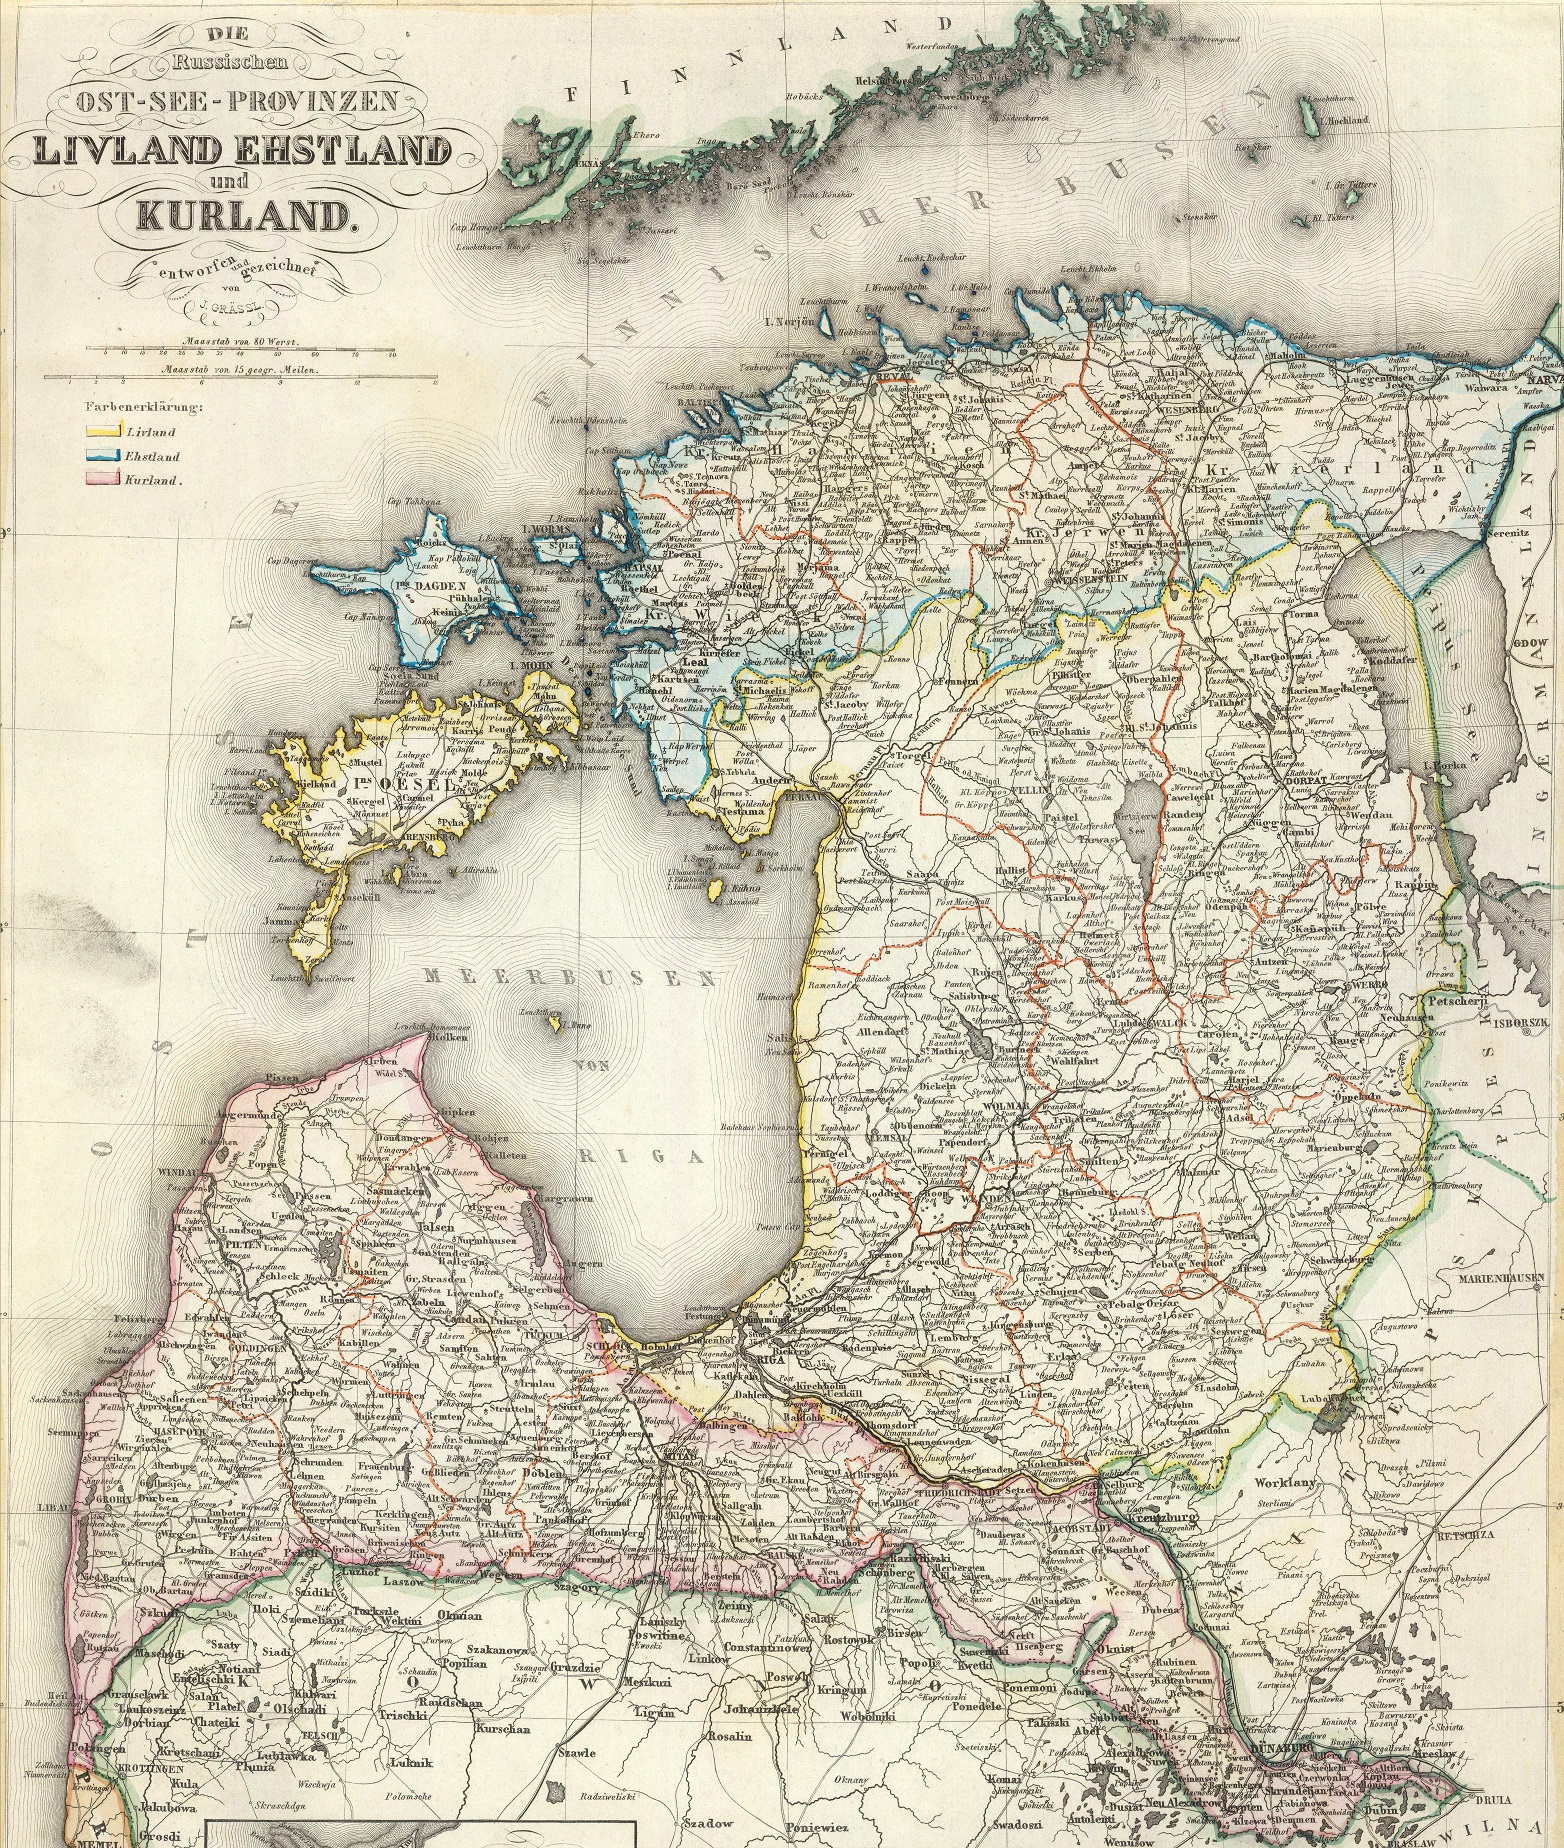
\includegraphics[width=0.9\linewidth]{images/provinces.jpg}
    \captionsetup{width=0.9\linewidth}
    \caption{Les gouvernements d’Estonie, Livonie et Curonie en 1860}
    \label{fig:provinces1860}
\end{minipage}
\begin{minipage}[b]{0.5\textwidth}
    \centering
    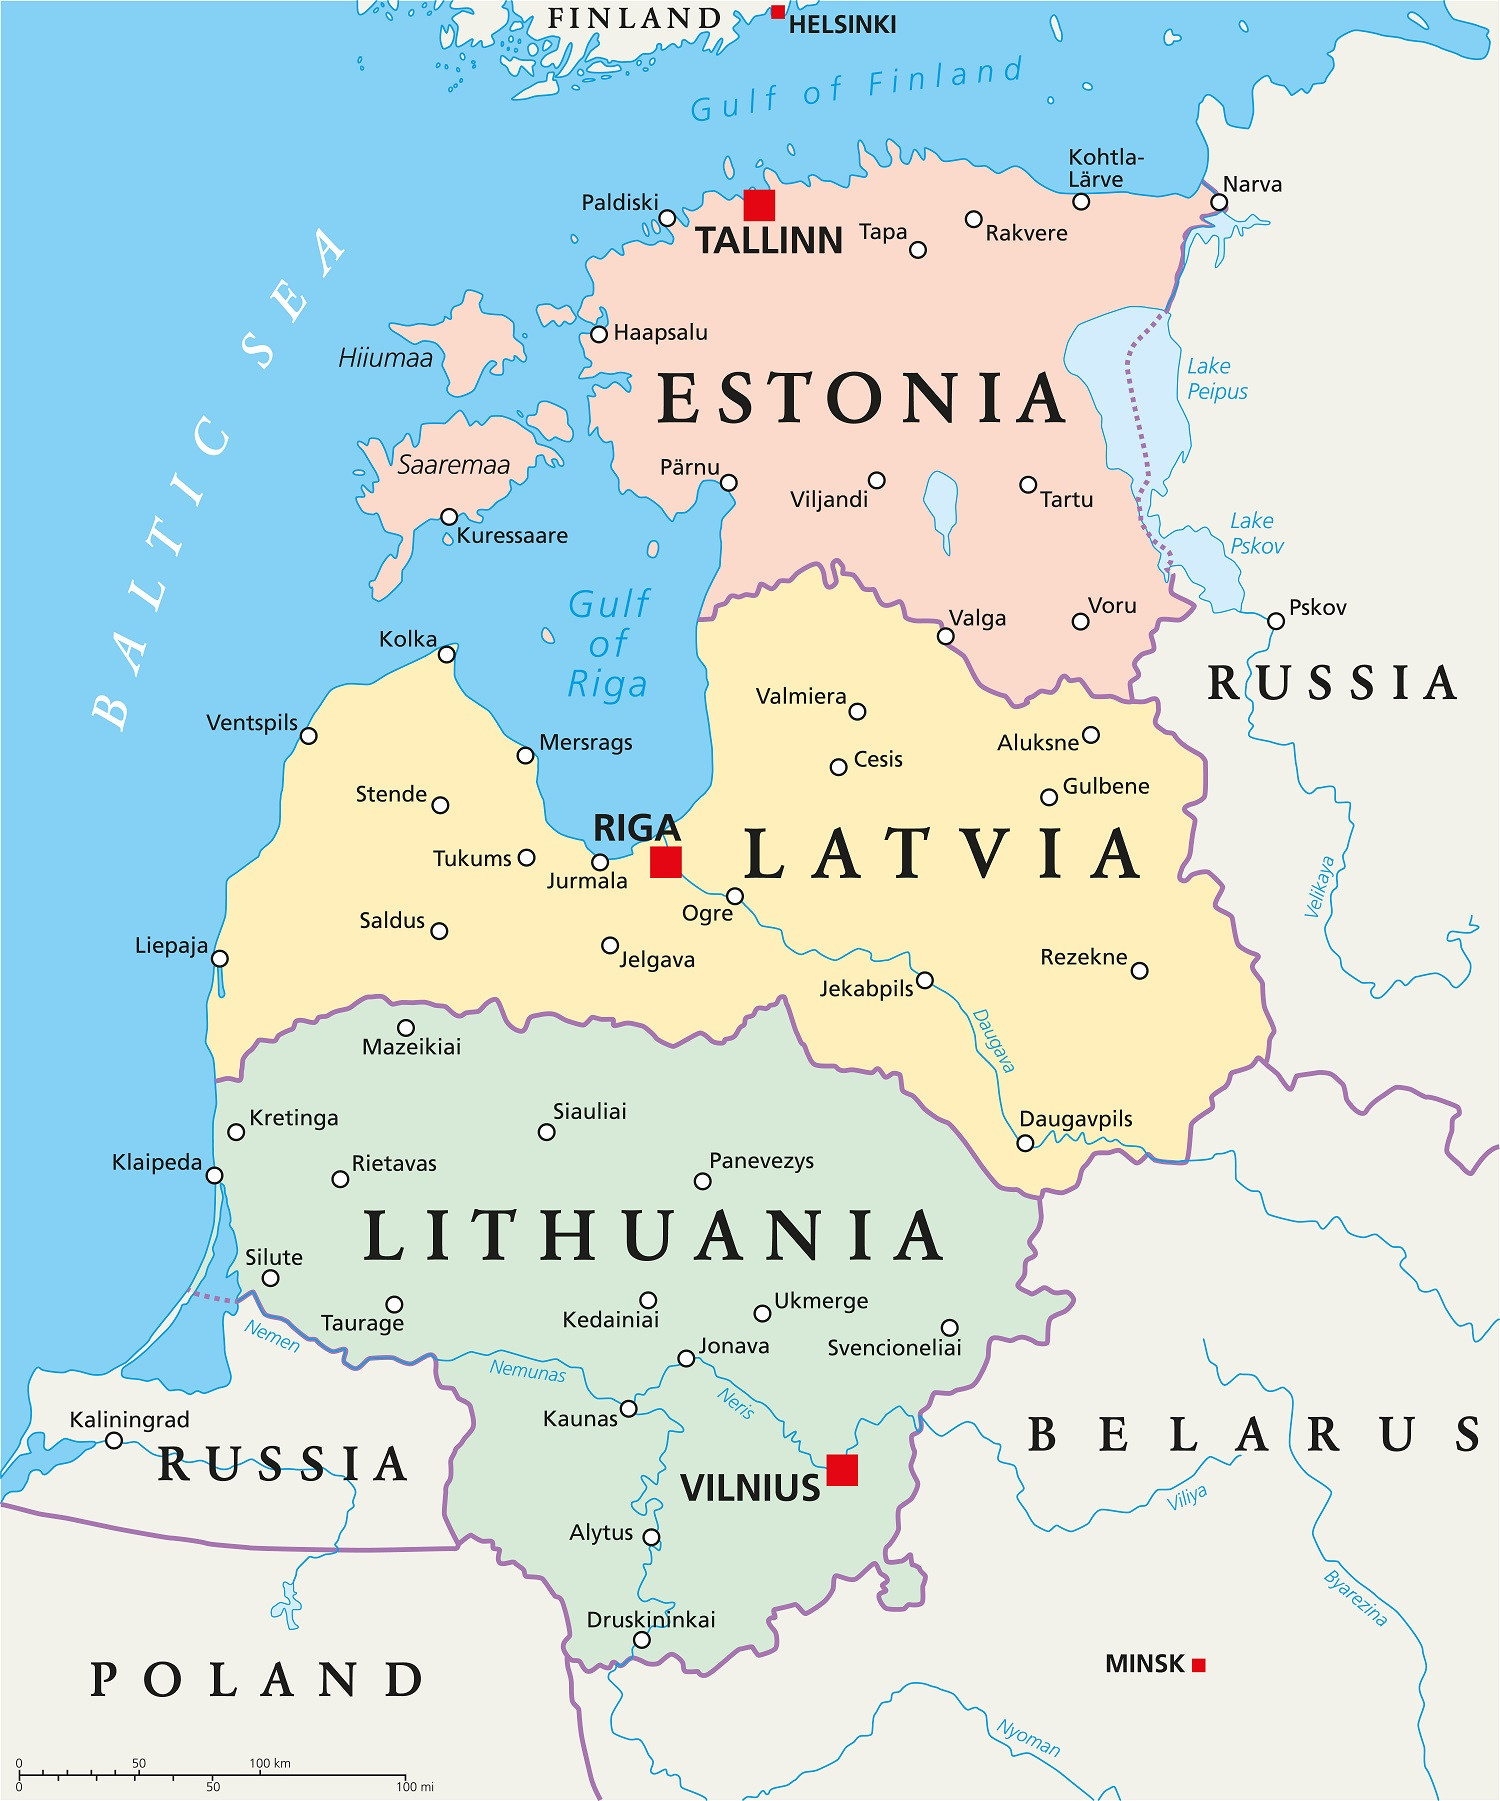
\includegraphics[width=0.9\linewidth]{images/balticcountries.jpg}
    \captionsetup{width=0.9\linewidth}
    \caption{L'Estonie, la Lettonie et la Lituanie aujourd'hui}
    \label{fig:balticcountries}
\end{minipage}
\end{figure}

Même après la dissolution de la Livonie médiévale au milieu du XVI\textsuperscript{e} siècle et les dépassements consécutifs de ses territoires entre les gros pouvoirs de la région - la Suède, la Russie et la Pologne -, la situation sociale de la région n'a changé que très peu.\footcites[Paradoxalement, l'allemand reste un élément unifiant à l'époque d'États-nations unitaires, au moins dans le domaine de l'historiographie. Les traitements scientifiques qui prennent en compte la région entière sous la forme et sous les critères qu'elle avait avant le XX\textsuperscript{e} siècle sont ainsi souvent publiés en allemand. Pour les relations internes et externes des pays baltes à partir du Moyen Age jusqu'à la fin du XIX\textsuperscript{e} siècle, cf. par exemple][]{anton_deutschland_2005}{angermann_baltischen_2015}{muhlpfordt_baltische_2016}{sommerlat-michas_baltikum_2015}{hormuth_livonia_2012} Ce n'était que au XIX\textsuperscript{e} siècle que la position de l'élite sociale et de la langue allemande fut progressivement contestée : d'un côté par les mouvements nationaux des Estoniens et Lettons qui avaient été libérés du servage en 1816-1819, et de l'autre par les ambitions croissantes de la Russie qui tentait d'imposer le russe comme la seule langue administrative dans toutes ses provinces vers la fin du siècle.\footcites[Les tensions culturelles et nationales entre les diverses peuples et minorités de la région, ainsi que leurs relations aux différents pouvoirs politiques externes sont les mieux présentées dans][]{angermann_ostseeprovinzen_2005}{plath_esten_2011} Cependant, l'allemand a conservé son statut de langue de la classe supérieure et moyenne privilégiée, même jusqu'à la première guerre mondiale. Ceci explique le choix des sources pour ce travail.

Les journaux allemands, publiés aux grandes et petites villes des gouvernements d'Estonie, Lettonie et Curonie offrent les meilleurs possibilités pour étudier le climat. Grâce à son statut en tant que \textit{lingua franca}, l'allemand ouvre une vue géographique et temporelle plus large. L'origine de la presse locale dans les gouvernements Baltes est situé aux années 1680, quand les premières gazettes hebdomadaires et bimensuelles ont parues à Riga et Reval (auj. Tallinn), les deux plus grosses villes baltiques.\footcites[][16-17]{vanamolder_was_2011}{peegel_eesti_1994} Au cours du 18\textsuperscript{e} et du XIX\textsuperscript{e} siècle, la masse de la presse a connu une croissance constante.\footcite[En 1813-1831, le nombre de revues publiées en Estonie et Livonie était 49; en 1831-1848 : 43, en 1849-1866 : 59; en 1867-1884 : 74.][301]{andresen_eesti_2010}

En général, le développement de la presse de langue allemande dans les pays baltes est similaire à celui du reste de l'Europe. Les magazines et les journaux étaient publiés par la bourgeoisie, les intellectuels et les nobles les plus libéraux. Ils étaient orientés vers le \og public \fg{} (\textit{Publizität}) en développement, qui devient un nouveau facteur important dans l'organisation de la vie sociale, en plus des structures de pouvoir existantes. Plusieurs journaux allemands baltes véhiculaient des idéaux des Lumières et étaient parfois polémiques sur les politiques impériales russes jugées rétrogrades (par exemple, concernant les droits des paysans).\footcite[][302-303]{andresen_eesti_2010} En ce qui concerne le contenu, ils publiaient principalement des rapports sur les affaires étrangères et des avis officiels (ukases impériaux, etc.) au début du siècle, mais ont commencé à inclure de plus en plus d'affaires locales vers le milieu du siècle. L'un des jalons à cet égard est le journal \textit{Das Inland}\label{das_inland}, publié à partir de 1836 à Tartu. Un autre changement important a été la politisation progressive de la presse, à partir de la fin des années 1850, les périodiques prenant des positions plus claires sur les affaires nationales et locales, malgré l'existence d'une censure.

Les quotidiens en estonien et en letton, en revanche, n'ont été publiés régulièrement que dans la seconde moitié du XIX\textsuperscript{e} siècle et diffèrent considérablement des journaux allemands. Comme le souligne Henrik Örnebring, le journalisme estonien (et par extension, letton) était avant tout au service de la prise de conscience nationale. Par rapport à la presse britannique, suédoise et allemande, les journaux estoniens et lettons étaient ancrés dans une tradition littéraire et éducative et avaient une division du travail très faible (un historien les a même qualifiés de \og presse à un seul homme \fg{} - \textit{Einmannpresse}).\footcite{ornebring_journalism_2013} Ces différences sont évidentes lorsqu'on examine les éditions contemporaines en allemand d'une part et en estonien ou en letton d'autre part. La portée thématique des journaux en langue allemande est beaucoup plus large et le ton est plus informatif, tandis que les journaux estoniens et lettons concentrent leurs efforts sur l'éducation de la population rurale (ils se sont aussi politisés progressivement, mais se concentraient principalement sur les affaires intérieures).

Le choix de se concentrer sur une seule revue, \textit{Rigasche Zeitung} est donc ancré dans le contexte historique du XIX\textsuperscript{e} siècle. Les revues germanophones paraissent de façon plus continue tout au long du siècle et couvrent un plus large éventail de sujets que leurs homologues estoniennes et lettones. Elles ressemblent aussi beaucoup à d'autres journaux contemporains du monde germanophone, ce qui ouvre une perspective pour des études comparatives à l'avenir. Dans les domaines voisins de la recherche en humanités numériques, il est également indéniable que la langue allemande offre beaucoup plus de possibilités d'analyse automatique. Bien que les approches finales adoptées dans ce mémoire n'utilisent pas de méthodes dépendantes de la langue (cf. la page \pageref{NER_approach} pour les considérations), une extension hypothétique de la recherche présentée ici pourrait très probablement faire appel à des applications de traitement du langage naturel (le domaine de recherche qui analyse le langage humain à l'aide de méthodes numériques). Au moment de la rédaction de ce mémoire, la technologie linguistique estonienne et lettone n'est pas tout à fait au niveau des grandes langues d'Europe occidentale, bien que les progrès soient remarquables en termes de proportion.

Enfin, il convient également de dire quelques mots sur la portée temporelle de la recherche. La période indiquée dans le sous-titre de l'ouvrage peut susciter la question \og pourquoi le XIX\textsuperscript{e} siècle ? \fg{} Premièrement, le XIX\textsuperscript{e} et XX\textsuperscript{e} siècles sont relativement négligés par les historiens du climat. D'une part, la plupart des chercheurs se sont occupés de la période qui précède les mesures météorologiques standardisées; et d'autre part les relations entre la société et le climat ne sont pas suffisamment explorées par les historiens de la modernité.\footcite[][11-12]{white_palgrave_2018} Dans le cas actuel, cela correspond aussi avec la disponibilité des sources. Plus précisément, l'analyse est menée avec les numéros du \textit{Rigasche Zeitung} de 1802 à 1888 (plus de détails à ce sujet dans le chapitre \ref{sources}), c'est-à-dire justement ce qui était facilement disponible sous forme numérisée. Ainsi, la période 1802-1888 pourrait soit être traitée comme une sorte de \og court XIX\textsuperscript{e} siècle \fg{}, soit être arrondie pour représenter le siècle entier.

Cependant, il y a aussi d'autres raisons pour lesquelles j'ai choisi de travailler avec cette source particulière, et sa correspondance approximative avec le XIX\textsuperscript{e} siècle était un argument important. Jürgen Osterhammel a écrit une analyse complète sur la définition du XIX\textsuperscript{e} siècle en tant que période historique. Il explique comment les tournants historiques correspondent rarement à des chiffres ronds du calendrier (comme les années 1800 ou 1900), mais considère néanmoins le XIX\textsuperscript{e} siècle comme une unité de recherche historique appropriée.\footcite[45-67]{osterhammel_transformation_2014} En comparant les différentes options de cadrage du siècle, il conclut : \og Dans l'ensemble, il y a de bonnes raisons de considérer le \og vrai \fg{} XIX\textsuperscript{e} siècle ou le XIX\textsuperscript{e} siècle  \og victorien \fg{} comme un tronc raccourci, c'est-à-dire, comme on l'a dit pour l'histoire allemande, \og une période de transition relativement brève et dynamique entre les années 1830 et 1890 \fg{} \fg{}.\footcite[][62-63]{osterhammel_transformation_2014}.

Il est possible d'interpréter la couverture temporelle des numéros numérisés du journal à l'aide du cadre défini par Osterhammel et d'autres. Bien que \textit{Rigasche Zeitung} ait été publié pour la première fois en 1778 et que des éditions numérisées soient disponibles à partir de 1802, le journal a commencé à évoluer à partir de sa forme moderne initiale au cours des années 1830. Comme démontré plus loin (cf. la figure \ref{fig:text_mass}), la fréquence de publication et la longueur moyenne des numéros ont commencé à augmenter au cours des années 1830, avant de devenir un quotidien en 1844.\footcite[Pour le nombre de numéros par an pendant toute la période de publication du journal, voir][220-222]{annus_eestis_1993} Cela signifie, par extension, que la majeure partie des données se situe entre les années 1830 et 1880, car les premiers numéros sont moins nombreux et plus courts. Les données des premières décennies sont néanmoins incluses dans l'analyse, en partie aussi parce que plusieurs des méthodes numériques utilisées fonctionnent mieux avec davantage de données.

L'extrémité supérieure de l'intervalle de temps coïncide bien avec la ligne tracée par Osterhammel. Il attribue une importance mondiale aux années 1880 pour de nombreuses raisons. Par exemple, il y a eu des changements importants dans l'utilisation de l'environnement (ce qui est particulièrement pertinent dans le contexte de ce sujet). L'utilisation de combustibles minéraux a dépassé celle de la biomasse pour la première fois, même si cela n'a pas affecté directement la majeure partie de la population mondiale. En outre, une nouvelle vague d'industrialisation a déferlé sur l'Europe et l'Amérique du Nord sous la forme de nouvelles inventions et d'une réorganisation de la production. L'empire russe connaît une croissance industrielle rapide à cette époque.\footcite[63-64]{osterhammel_transformation_2014} Dans les provinces baltes, les premières lignes télégraphiques avaient été posées dans les années 1850 et la construction de chemins de fer avait commencé dans les années 1860. Ces nouvelles technologies, ainsi que les changements sociaux (émancipation progressive et mobilité accrue de la population rurale) ont contribué à l'établissement de nombreuses nouvelles usines dans les dernières décennies du siècle.\footcite[154-161]{andresen_eesti_2010}





\subsection*{Questions de recherche} \label{questions}
\addcontentsline{toc}{subsection}{Questions de recherche}

La nature de la recherche en question est exploratoire. A l'origine, je m'étais engagé sur une voie plus étroite et j'avais essayé d'automatiser la détection et l'encodage des descriptions du temps pour les intégrer automatiquement dans le cadre d'Euro-Climhist. Cela a donné lieu à plusieurs tentatives qui ont été partiellement développées mais non incluses dans cette version finale du travail. Plus particulièrement, j'ai expérimenté la géolocalisation automatique des événements météorologiques - un système qui trouverait des noms de lieux à l'intérieur du texte et les connecterait à des coordonnées sur une carte, donnant ainsi un aperçu géographique des descriptions météorologiques dans les sources. Il s'agissait d'une tâche difficile, notamment parce que je voulais limiter l'étendue spatiale à la région baltique et que les lieux de cette région étaient généralement désignés par leur nom allemand au XIX\textsuperscript{e} siècle, alors que les bases de données modernes qui permettent de relier les noms aux coordonnées contiennent des noms estoniens et lettons. La tentative a été modérément réussie, mais je l'ai abandonnée pour plusieurs raisons.

Tout d'abord, je me suis intéressé davantage aux descriptions qu'aux événements eux-mêmes. Comme expliqué ci-dessus, connaître les types de contextes qui peuvent entourer (et influencer) les informations climatiques conduira à une interprétation plus précise et à un encodage possible de celles-ci. Deuxièmement, dans ce contexte, une focalisation spatiale sur la région baltique ne semblait plus raisonnable, étant donné que les informations trouvées dans les journaux étaient internationales par nature, appartenant plus largement à la germanosphère, mais incorporant également des informations directes provenant du français, de l'anglais, du russe et d'autres langues via des informations traduites. Il était évident que le \textit{Rigasche Zeitung} s'inscrivait ainsi dans le schéma beaucoup plus large du \og discours climatique \fg{} du XIX\textsuperscript{e} siècle. D'une certaine manière, la presse européenne de l'époque peut être imaginée comme une boîte avec de nombreuses ouvertures. La lecture d'un journal peut offrir une vision légèrement différente de celle d'un autre, mais il s'agit toujours d'un regard à l'intérieur du même système.

L'approche plus large permet également d'expérimenter des méthodes qui peuvent potentiellement être appliquées à d'autres sources que le \textit{Rigasche Zeitung}, soit pour élargir les conclusions présentées dans ce travail, soit pour nuancer les différences régionales qui peuvent apparaître dans la presse. Mais surtout, elle augmente la valeur de ce mémoire, car les conclusions ne s'appliquent pas seulement à un journal ou à une région en particulier, mais nous donne des indices sur le discours climatique dans toute l'Europe au XIX\textsuperscript{e} siècle. En gardant cela à l'esprit, ainsi que les considérations historigraphiques et méthodologiques présentées ci-dessus, les deux axes principaux de recherche de ce mémoire sont donc les suivants :

\vspace{1ex}
\begin{enumerate}
    \item Application des méthodes des humanités numériques dans la recherche sur l'histoire du climat, notamment à l'étape de l'extraction de données :
    \begin{itemize}[label=$\bullet$]
        \item L'exploration des données - description, analyse et visualisation des sources afin de donner un contexte aux étapes suivantes ;
        \item Détection des mentions de phénomènes météorologiques individuels dans les textes, quantifier et comparer leurs occurrences sur une échelle temporelle ;
        \item Analyse des relations sémantiques entre les différents phénomènes météorologiques et les mots liés au temps ;
        \item Modélisation computationnelle des contextes qui entourent les mentions du climat et du temps ;
        \item La comparaison et la visualisation de ces \og sujets du climat \fg{}, tant sur le plan sémantique que temporel ;
        \item Réflection sur le potentiel et les limites des méthodes proposées.
    \end{itemize}
    
    \item Discussion des résultats pour proposer des explications préliminaires de la relation entre la société et le climat telle que reflétée dans les sources :
    \begin{itemize}[label=$\bullet$]
        \item Contextualisation historique des sources ;
        \item Précision de la position du journal imprimé comme source d'histoire du climat au XIX\textsuperscript{e} siècle (cf. le tableau \ref{tab:source_types}) ;
        \item Analyse des tendances de mentions des phénomènes météorologiques dans les sources ;
        \item Exploration les contextes dans lesquels on parle du temps ;
        \item Proposition d'idées pour des recherches futures.
    \end{itemize}
\end{enumerate}
\vspace{1ex}
\clearpage

Les étapes nécessaires pour traiter ces questions et leur ordre sont présentées dans la figure \ref{fig:workflow}.

\begin{figure}[h]
    \centering
    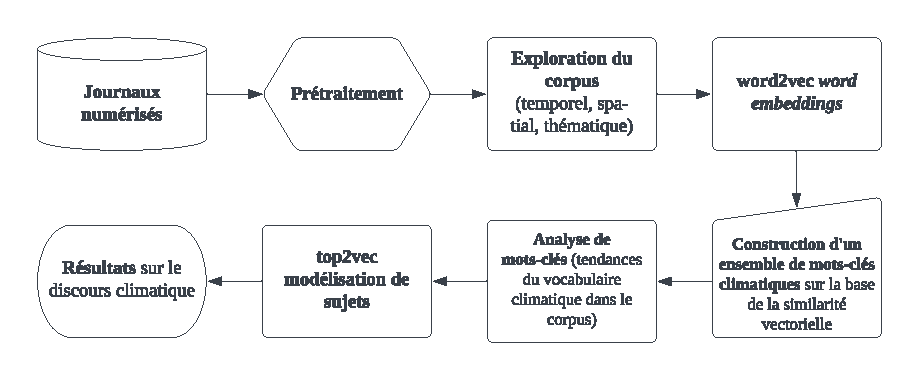
\includegraphics[width=0.95\textwidth]{images/workflow_FR.pdf}
    \caption{Diagramme des étapes de travail}
    \label{fig:workflow}
\end{figure}


La structure de ce mémoire est composée de trois chapitres principaux. Le premier chapitre est entièrement consacré aux sources et n'aborde pas encore directement le climat. L'objectif est plutôt de décrire les caractéristiques générales du journal qui sont la toile de fond de toutes les analyses ultérieures de son contenu lié à la météo. Il comprend également une sous-section sur le prétraitement, c'est-à-dire la systématisation et le nettoyage des données nécessaires à des analyses efficaces par la suite. Le deuxième chapitre examine les informations météorologiques et climatiques dans les sources au niveau des mots simples et introduit une nouvelle méthode pour faire converger différentes formes de mots grammaticales et orthographiques vers des formes normalisées. Le chapitre procède ensuite à la démonstration des possibilités d'analyse de ces mots individuels et de leurs fréquences. Dans le troisième chapitre, l'attention est élargie aux mots individuels au contexte qui les entoure. Avec les méthodes de modélisation thématique, les textes autour de ces mots sont automatiquement catégorisés en un certain nombre de types ou \og sujets \fg{}, qui sont ensuite analysés et nommés (avec des détails plus précis sur chaque thème présentés en annexe). Des conclusions et des idées mineures sont présentées au cours de l'analyse avec des résumés intermédiaires à la fin de chaque chapitre principal. Une discussion finale des résultats, des limites et des perspectives futures se trouve dans la conclusion.

\medskip

Le mémoire contient une bonne part d'allemand, car c'est la langue des sources. J'ai fait de mon mieux pour transmettre toutes les informations nécessaires aux lecteurs qui ne le maîtrisent pas, que ce soit dans des tableaux, des parenthèses ou des notes de bas de page. Il y a cependant un certain va-et-vient entre le français et l'allemand, et j'espère que cela n'empêche pas une lecture confortable du mémoire. Un autre élément caractéristique de cette recherche est la combinaison des méthodes numériques avec celles de l'histoire. J'ai décidé de renoncer à un chapitre séparé pour les méthodes et de les introduire plutôt au fur et à mesure que la recherche se développe, aux moments nécessaires. De manière générale, cependant, il faut dire que toutes les manipulations numériques rencontrées dans ce travail sont réalisées avec le langage de programmation Python qui est très bien adapté à toutes sortes de tâches d'analyse de données et d'apprentissage automatique. Python dispose d'un grand nombre de bibliothèques et de modules téléchargeables gratuitement et qui peuvent être facilement intégrés au reste du code, afin de réaliser des tâches spécifiques telles que la modélisation de sujets, par exemple. J'ai essayé de décrire ces techniques et concepts numériques spécifiques de la façon la plus simple possible, en imaginant s'adresser à un lecteur novice plutôt qu'expert. Les lecteurs plus aguerris aux approches computationnelles pourront se plonger dans la documentation de l'un ou l'autre module via les liens fournis dans les notes de bas de page. Pour ceux qui souhaitent reproduire les résultats ou simplement suivre de près les approches adoptées, tout le code et les \textit{notebooks} sont disponibles sur la page GitHub du projet.\footnote{\url{https://github.com/krkryger/clim-dist}} Les données brutes et les modèles entraînés, trop volumineux pour être hébergés dans sur GitHub, sont disponibles en téléchargement en me contactant.

\clearpage



\section{Sources} \label{sources}

\subsection{Description} \label{description_corpus}

% natuke RZ-st ?

Les données mobilisées par ce mémoire sont des numéros numérisés du journal \textit{Rigasche Zeitung} (\og le journal de Riga \fg{}). Le journal a été publié pour la première fois en 1778 par Georg Ludwig Zachariae sous le nom de \textit{Rigische Politische Zeitung}.\footcite[Les éditeurs suivants au XIX\textsuperscript{e} siècle ont été Julius Conrad Daniel Müller (de 1808 à 1830) ; Heinrich Steffenhagen (1830 - ?) ; Adolf Müller ( ? - 1877) ; Georg Berkholz et Joh. Ad. Kröger (1877 - 1885) ; J. A. Kröger et J. C. Schwartz (1885 - 1889).][220]{annus_eestis_1993} À partir de 1801, il a porté le nom de \textit{Rigasche Zeitung} et a été publié sans interruption jusqu'en 1889. La publication a ensuite cessé jusqu'en 1907, date à laquelle elle a été reprise et poursuivie jusqu'en 1915.\footcite[220-222]{annus_eestis_1993} Dans les années 1840, le \textit{Rigasche Zeitung} est devenu le plus important quotidien de la région balte.\footcite[303]{andresen_eesti_2010}

Les éditions numérisées proviennent des collections de la Bibliothèque nationale lettone (LNB).\footnote{\url{https://lnb.lv/en}} En comparaison à la Bibliothèque nationale estonienne\footnote{\url{https://nlib.ee/en}} où se trouvent également plusieurs journaux gérmanophones du XIX\textsuperscript{e} siècle, leur collection est considérablement plus vaste, car Riga était le centre économique et le capitale \textit{de facto} des gouvernements Baltes. La partie principale de la numérisation des collections de l'LNB a été terminée vers 2012. Pour les journaux, les paramètres du balayage étaient JPEG 2000 et 400 dpi. Remarquablement, la segmentation des milliers de pages pour l'océrisation a été faite à la main.\footnote{\url{https://lndb.wordpress.com/2012/06/07/periodikas-digitalizesana-lnb/}}

LNB offre un accès libre à toutes les revues et gazettes du XIX\textsuperscript{e} siècle sur la page web periodika.lv\footnote{\url{periodika.lv}}, ainsi qu'un moteur de recherce textuelle pour les transcriptions, mais il n'est pas possible de les télécharger (par exemple sous la forme d'une API). Par conséquent, il a été nécessaire de contacter la bibliothèque pour recevoir le corpus. Pour le travail de la première année de master, un corpus d'une plus petite taille (ca. 33 000 articles) et avec des critères additionnels (notamment la présence des certains mots clés météorologiques) a été utilisé. Ce corpus a été en suite utilisé pour expérimenter des approches différentes et nombre d'entre eux ont trouvé son chemin vers ce travail-ci pour être appliquées à un corpus plus vaste.

Le jeu de données utilisé pour ce mémoire (désormais le corpus LNB) est composé de \textbf{289 704 articles} du \textit{Rigasche Zeitung} de 1802 à 1888.\footnote{\texttt{./data/external/riga\_zeit\_1802\_1859.parquet \newline ./data/external/riga\_zeit\_1859\_1888.parquet}} Les articles se répartissent sur 18 499 numéros du journal au cours de 86 ans.\footnote{En fait, il y a 87 années de 1802 à 1888, mais l'an 1882 n'est pas présent dans la base de données de LNB, comme on peut le voir sur les pages suivantes. Le journal était bien publié continuellement - il s'agit d'une lacune de la numérisation. \label{86_years}} Un aperçu de la distribution des données se présente dans la figure \ref{fig:data_hist}.

\begin{figure}[t]
    \centering
    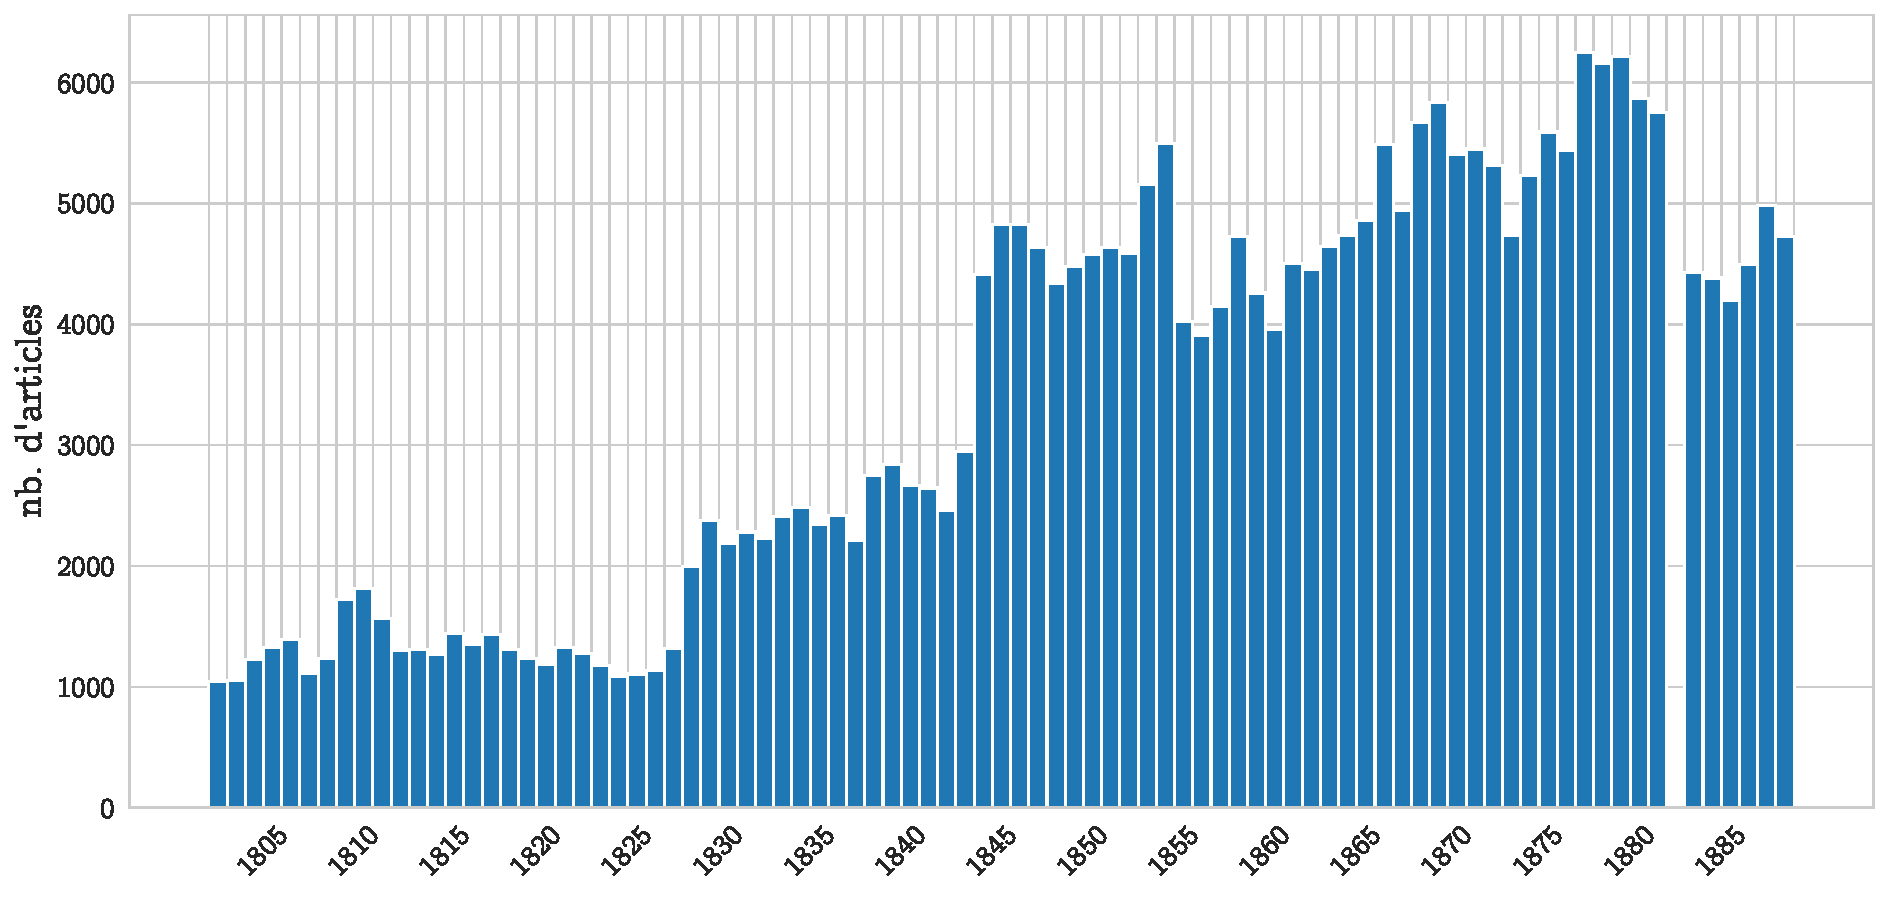
\includegraphics[width=\textwidth]{images/articles_histogram.pdf}
    \caption{Distribution temporelle des données}
    \label{fig:data_hist}
\end{figure}

Dans ce corpus, chaque entrée corréspond à un article et est fournie des caractéristiques suivantes (voir les annexes pour un exemple des données brutes) :

\vspace{1ex}
\begin{itemize}[label=$\bullet$]
    \item \texttt{href} : le lien vers l'article sur \url{periodika.lv} qui permet de vérifier la transcription (mais qui, selon mon expérience précédente avec le site, n'est malheureusement pas permanent et peut être sujet à changement)
    \item \texttt{head} : le titre de l'article
    \item \texttt{date} : la date de publication (selon le calendrier Julien qui était le calendrier officiel de l'Empire russe jusqu'à 1915 en Lettonie et 1918 en Estonie)
    \item \texttt{pub} : le nom de la revue
    \item \texttt{full\_text} : la transcription OCR de l'article entier
    
\end{itemize}
\vspace{1ex}

Enfin, l'index des entrées du corpus brut est utilisé de manière continue tout au long du travail. Cet index, référencé comme \texttt{id}, permet de retracer tout texte jusqu'à sa forme originale au cours des différentes procédures d'analyse, en le reliant à ses métadonnées. Dès lors, les références aux articles du \textit{Rigasche Zeitung} sont accompagnées de ses \texttt{id} correspondants dans les notes de bas de page, ce qui permet de les retrouver plus facilement dans le corpus.\label{id_indexing}

\subsection{Prétraitement}  \label{pretraitement}

Avant de passer à l'analyse thématique, un traitement et nettoyage préliminaire du corpus sont nécessaires. Le prétraitement consiste à générer des caractéristiques supplémentaires pour pouvoir sélectionner et manipulation plus aisément, et à traiter le texte brut en le séparant en mots singuliers pour permettre la vectorisation et l'analyse des mots-clés.

Le premier prétraitement des données a été réalisé avec la bibliothèque Pandas de Python qui permet de faire toute sorte de manipulation sur des tableaux. Les attributs suivants ont été dérivés à partir des existants et ajoutés au corpus\footnote{{\texttt{./climdist/data\_preprocess.py}, fonction \texttt{basic\_preprocess}}} :

\vspace{1ex}
\begin{itemize}[label=$\bullet$]
    \item \texttt{year} : l'année
    \item \texttt{month} : le mois
    \item \texttt{day} : le jour
    \item \texttt{text\_len} : le nombre des caractères dans \texttt{full\_text}
\end{itemize}
\vspace{2ex}

\subsubsection{Evaluation de la qualité d'OCR} \label{ocr_quality}

Ensuite, les textes avec une qualité trop faible ont été marqués pour pouvoir les écarter aux stades de l'analyse textuelle. Le tableau \ref{table:ocr} montre une échantillon de texte tel que visible sur le site de LNB et son OCR correspondante (les erreurs sont surlignées en jaune). Bien entendu, la qualité peut varier considérablement entre les textes ou dans un seul texte, mais cet exemple illustre bien certains des problèmes habituels. On peut constater plusieurs choses. Premièrement, le journal utilise l'écriture gothique (\textit{Frakturschrift}) qui pose normalement plus de défis pour un moteur OCR.\footcite[Pour un aperçu des problématiques généraux de l'OCR des textes allemands (quoique avec un accent sur les XVII\textsuperscript{e}-XVIII\textsuperscript{e} siècles) et pour l'état de l'art autour du moment de la complétion de la numérisation des catalogues de LNB, cf. ][]{federbusch_volltext_2013} Ces difficultés se présentent le plus souvent sous la forme de confusion de \textit{f} avec \textit{s}, et le groupe \textit{m}, \textit{n}, \textit{e}, \textit{tt} et \textit{ii}. En plus, les guillemets \og \fg{} apparaissent souvent sans raison. Deuxièmement, la segmentation des articles et très étroite, un fait qui cause des problèmes aux bouts de lignes. Ainsi, les tirets de césure sont très souvent omis du texte résultat, provoquant beaucoup d'ambiguïté par rapport aux mots composés (omniprésents en allemand). Un autre problème lié à la segmentation n'est pas visible dans l'exemple mais se présente dans le cas d'une mise en page complexe : les limites d'un article peuvent être flous ou se confondre avec des publicités ou d'autres éléments.

\begin{table}[h]
\begin{minipage}[b]{0.415\textwidth}
    \centering
    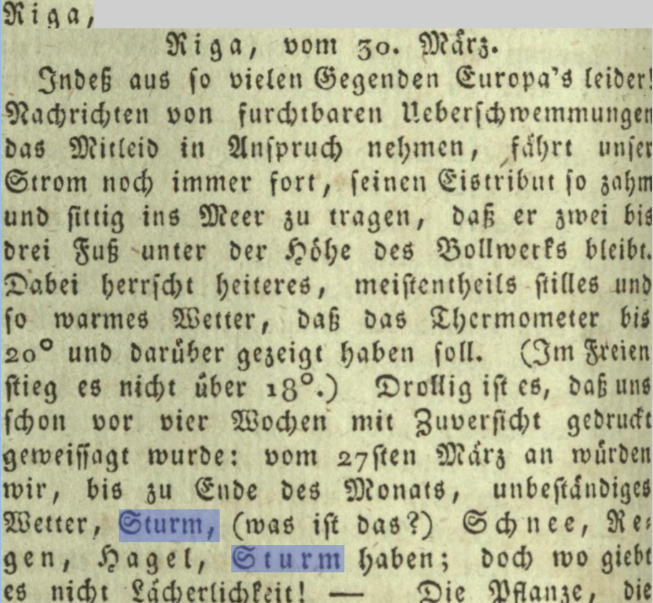
\includegraphics[width=\linewidth]{images/ocr_comparaison.png}
  \end{minipage}
  \hspace{0.05\textwidth}
  \begin{varwidth}[b]{0.5\textwidth}
    \centering
    \scriptsize
      \parbox[b]{\linewidth}{\texttt{Riga\\\\\hl{P}i\hl{s}a, vom \hl{so. Wirst-z. \fg{}} \\ \hl{\fg{} Jtt}deß aus so vielen Gegenden E\hl{n}ropa\hl{w} leider!\\
Nachrichte\hl{tt} von furchtbaren \hl{Il}eberschwe\hl{tnnt}u\hl{tt}gen\\
das Mitleid in Anspruch nehmen, \hl{\fg{}sti}hrt \hl{ti}nse\hl{t}\\
Strom noch immer fort, \hl{f}einen Eistri\hl{lsti}t so zahm\\
und\hl{\fg{}} sittig ins Meer zu tragen, daß er zwei bis\\
drei\hl{\fg{}} Fuß \hl{\fg{}}unter der Höhe des \hl{V}ollwerks bleibt.\\
Dabei herrscht heiteres, meistentheils stilles und\\
so warmes Wetter, daß das Thermo\hl{sn}eter bis\\
\hl{no\fg{}} und darüber gezeigt haben soll. (\hl{Jtn} Freien\\
stieg es nicht über \hl{:80}.) Drollig\hl{\_}ist\hl{\_}es, daß\hl{\_}utts\\
schon vor vier Wochen mit Zuversicht gedruckt\\
geweissagt wurde: vom 27\hl{f}ten M\hl{ei}rz an würden\\
wir, bis zu Ende des \hl{Nk}onat\hl{th} unbes\hl{icktt}diges\\
Wetter, Sturm, (\hl{tv}as ist das?) Schnee, \hl{N\fg{}}\\
gen, Hagel, Sturm haben; d\hl{v}ch w\hl{v} giebt\\
es nicht \hl{\fg{}}Lächerlichkeit! —\hl{\fg{}} Die Pflanze, die}}
  \end{varwidth}%
  \caption{Exemple de la qualité d'océrisation de LNB}
  \label{table:ocr}
\end{table}

La post-correction d'un corpus historique est considérée comme une tâche très ardue, bien que ce domaine soit en plein développement.\footnote{Pour une comparaison d'approches et l'état d'art, cf. Gotscharek Annette, Reffle Ulrich, Ringlstetter Christoph, Schulz Klaus U. et Neumann Andreas, 2011, \og Towards information retrieval on historical document collections: the role of matching procedures and special lexica \fg{}, International Journal on Document Analysis and Recognition (IJDAR), juin 2011, vol. 14, n. 2, p. 159‑171.} Un nettoyage complet des données serait donc hors du champ de ce travail. Il est cependant possible d'arriver à des résultats significatifs en utilisant la taille même du corpus et en reconnaissant ses limitations d'OCR. Au lieu d'attendre une océrisation \og parfaite \fg{}, nous pouvons faire usage des qualités existantes du texte. Pendant des expérimentations, il s'est avéré que les approches de traitement automatique de la langue (\textit{Natural Language Processing}, NLP) ont bien des limitations, mais peuvent être utilisés conjointement avec des méthodes \textit{corpus-based}, notamment ceux qui s'appuient sur des vecteurs de mots que nous verrons plus tard.

A place d'une post-correction des textes, j'ai donc décidé d'implémenter un simple algorithme d'apprentissage machine afin de pouvoir écarter les entrées d'une trop mauvaise qualité pour l'étape d'analyse textuelle. Toutes les données sont conservées pendant ce stade, mais chaque entrée est fournie d'une score (\texttt{0} ou \texttt{1}) pour permettre d'établir un taux de \og lisibilité \fg{}. Afin d'entraîner un modèle d'apprentissage supervisé, un nombre de textes sont traités en Python par un modèle de langue allemande développé par SpaCy.\footnote{Pour cette analyse simple et préliminaire, un modèle de base \texttt{de\_core\_news\_md} est utilisé, entraîné sur des textes allemands contemporains. Les détails du modèle se trouvent ici : \url{https://spacy.io/models/de\#de\_core\_news\_md}\label{de_core_news}} Le modèle est utilisé ici pour \textit{tokeniser} le texte, i.e. itérer un séquence de caractères et d'en repérer leur structure, en séparant les mots les uns des autres et en ajoutant à chaque mot (token) des étiquettes qui décrivent leur position morpho-syntaxique. A ce point nous ne nous intéressons qu'aux quantités relatives des différents types de tokens dans le texte. Les caractéristiques sélectionnées pour chaque texte, afin de le classifier selon la lisibilité, sont les suivantes :
\vspace{1ex}
\begin{itemize}[label=$\bullet$]
    \item proportions relatives des étiquettes morpho-syntaxiques suivantes: pronom, adverbe, auxiliaire, nombre, verbe, adjectif, espace, ponctuation, inconnu;\footnote{\textit{Ibid.} pour la schéma d'annotation morpho-syntaxique du modèle en question.}
    \item proportion relative de symboles \og inhabituels \fg{}, n'appartenant pas à \textit{a-z}, \textit{A-Z} (y compris les caractères spéciaux \textit{öäüß} de la langue allemande) ou le groupe \mbox{\textit{.,'"?!;-:}}
    \item nombre de caractères divisé par le nombre de tokens
\end{itemize}
\vspace{2ex}

Pour apprendre un modèle d'apprentissage machine à distinguer les textes lisibles de ceux qui contiennent trop de bruit ou d'erreurs à partir des caractéristiques nommées, une échantillon aléatoire de 300 textes est sélectionné et chaque texte est évalué. Les textes considérés illisibles sont ceux qui en pratique ne pourraient jamais être proprement traités par l'ordinateur (ou qui ne sont même pas compréhensibles pour l'humain - voir le tableau \ref{tab:readability_example} pour un exemple de texte considéré illisible. Le texte dans le tableau \ref{table:ocr} aurait un score positif).

\begin{table}[h]
\centering
\begin{tabular}{|p{0.9\linewidth}|}
\hline
\vspace{0.5ex}
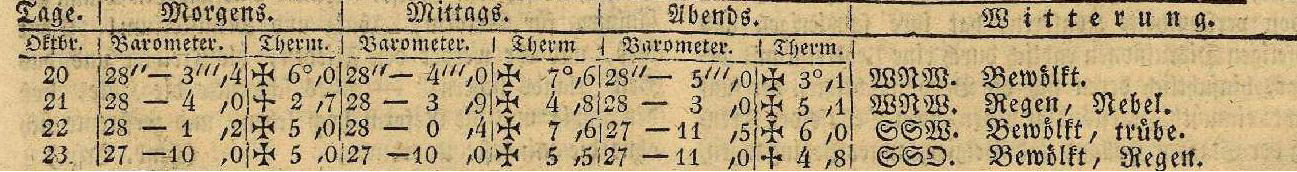
\includegraphics[width={\linewidth}]{images/ocr_quality_example.png} \\
\hline
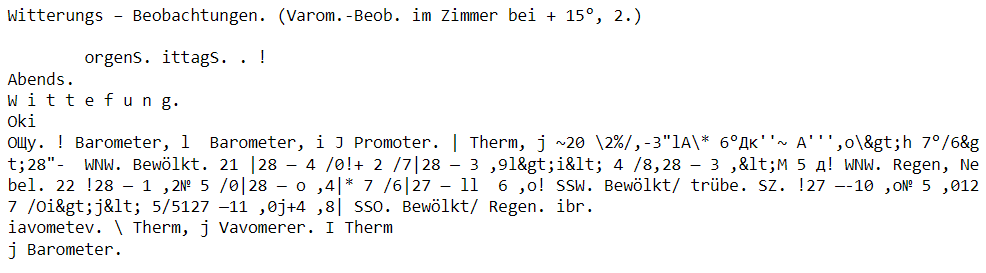
\includegraphics[width={\linewidth}]{images/ocr_quality_example_text.png} \\
\hline
\end{tabular}
\captionsetup{justification=centering}
\caption{Extrait d'un article considéré illisible dans le \textit{ground truth}\\ (RZ 24/10/1831 (\texttt{id: 42181}))}
\label{tab:readability_example}
\end{table}

Les caractéristiques et les annotations pour ces 300 textes sont ensuite utilisées comme les données d'entraînement d'un classificateur de type machine à vecteurs de support (SVM).\footnote{L'annotation et l'entraînement se trouvent dans \texttt{./notebooks/ocr\_quality.ipynb}} La machine à vecteurs de support a pour but de projeter chaque point de données dans un espace hyperdimensionnel (dont le nombre de dimensions correspond au nombre de caractéristiques énumérées ci-dessus) et de trouver un hyperplan qui sépare le deux groupes de données (i.e. lisibles et non lisibles) en maximisant la distance entre chaque point d'entrée et l'hyperplan.\footcite{suthaharan_support_2016}

L'exactitude moyenne atteinte par le modèle s'élève à 87\%, un score dont la signifiance est difficile à évaluer, étant donné la nature subjective du classificateur. La décision sur la lisibilité d'un texte est faite par un algorithme mais elle repose pourtant sur un élément subjectif, car c'est l'utilisateur qui établit la norme (\textit{ground truth}) que l'algorithme essaie de reproduire.
Il est impossible d'établir une frontière bien délimitée entre lisible et non lisible - deux catégories dont la distinction reste intrinsèquement fluide - mais l'on peut dire avec une certaine confiance que l'application du classificateur aide à nettoyer le corpus et la perte de données d'une qualité haute d'OCR est presque inexistante.\footnote{Le classificateur se trouve dans \texttt{./data/models/ocr\_quality\_model/}, le script pour l'appliquer à tout le corpus et générer la colonne de lisibilité est \texttt{./climdist/ocr\_quality.py}}

\begin{figure}[h!]
\centering
\captionsetup{justification=centering}
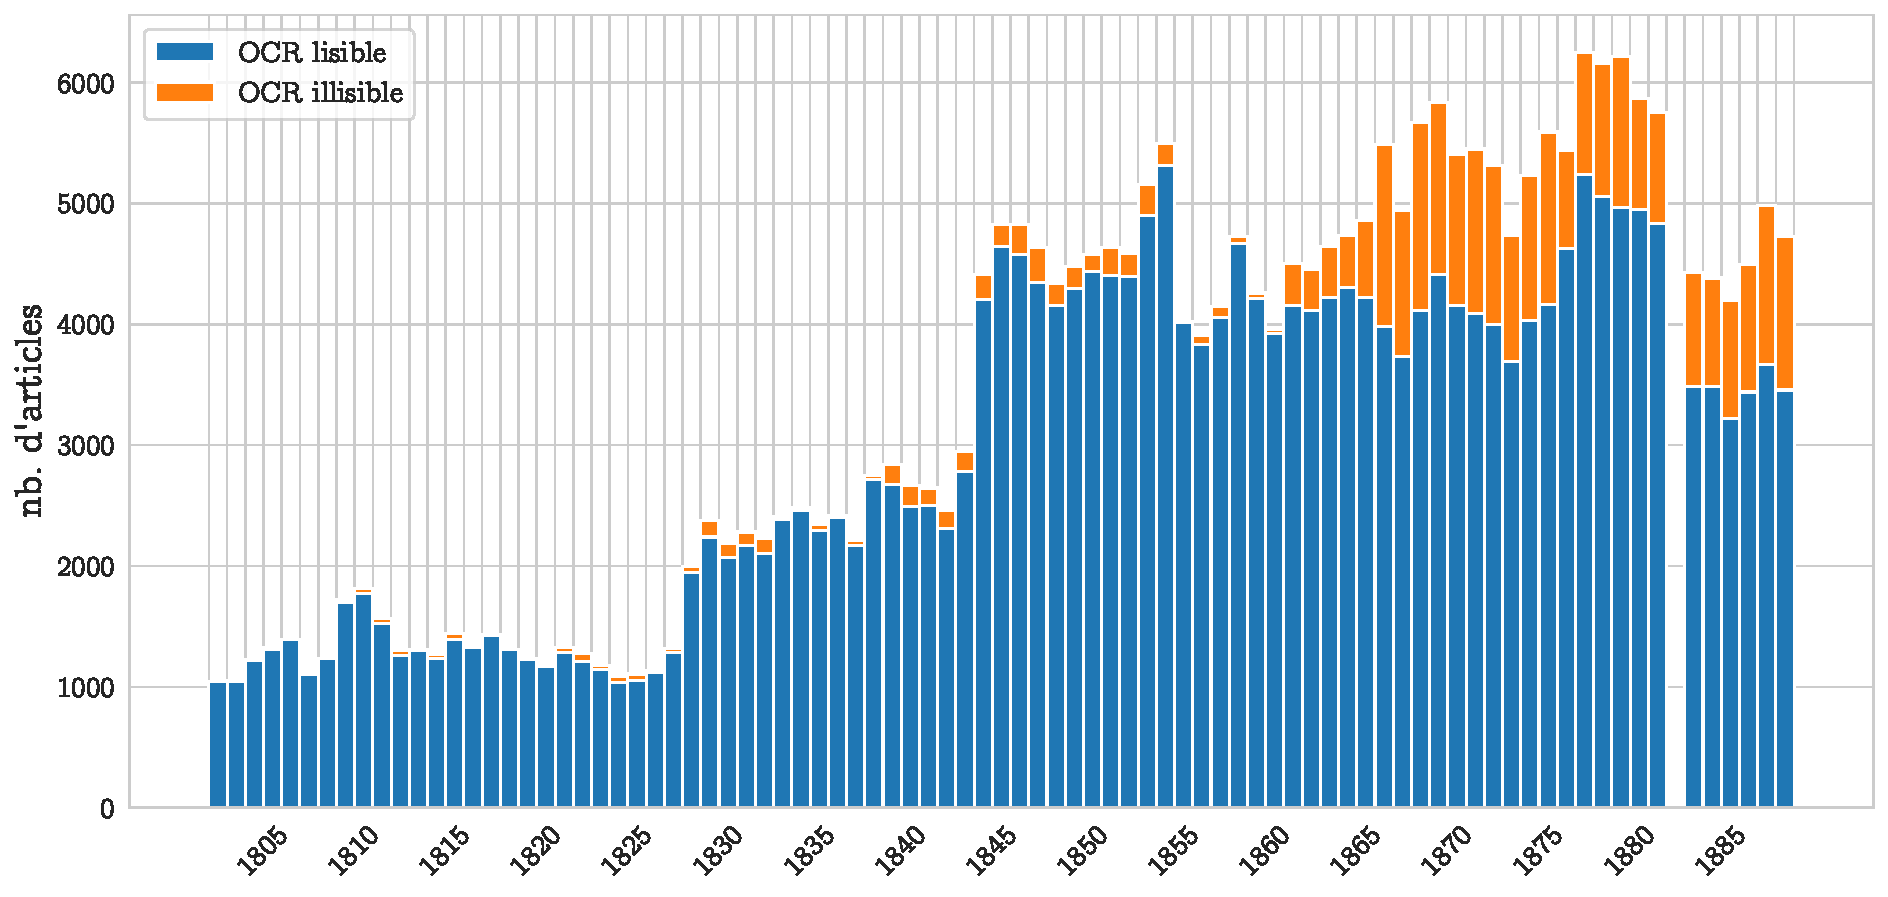
\includegraphics[width=\textwidth]{images/readability_histogram.pdf}
\caption{Distribution temporelle des données et la proportion d'articles classifiés illisibles}
\label{fig:readability_hist}
\end{figure}

Au total, 32 709 articles, soit 11\%, du corpus entier, sont considérés illisibles par le modèle SVM. Leur distribution temporelle dans le corpus, présenté sur la figure \ref{fig:readability_hist}, nous donne quelques informations sur les types d'articles qui sont normalement d'une mauvaise qualité d'OCR. La proportion de textes illisibles reste très faible jusqu'aux années 1860, d'où elle augmente considérablement. Mais c'est exactement à ce moment que la nature du journal est en plein changement - l'on voit l'apparition de nouvelles rubriques employant des nouvelle structures de l'information. Cela sera traité plus en détail sur la page \pageref{beobachtungen_riga}.

\subsubsection{Tokenisation} \label{tokenisation}

Après la classification des textes selon leur lisibilité, le contenu des articles est séparé en mots singuliers.\footnote{\texttt{./climdist/tokenize.py}} Cette tâche est accomplie par une méthode assez simple. D'abord, les textes sont séparés par des espaces. Ensuite, chaque part est mise en minuscule et les symboles de ponctuation sont enlevés des deux côtés (cela a pour but de supprimer les virgules et les points, mais aussi les guillemets erronés qui apparaissent souvent). Puis, chacun de ces \og mots \fg{} est évalué par une fonction qui compare la proportion de caractères réguliers dans le mot à la proportion de ponctuation, de chiffres et de caractères non latins au milieu du mot (des caractères cyrilliques sont parfois présents). La valeur maximale autorisée pour ces symboles peu courants a été fixée à 30\% pour ne pas perdre trop de l'information. Les \textit{stopwords}, i.e. les articles, les mots \og connecteurs \fg{} et les mots qui sont les plus courants dans la langue mais dont le sens , sont également écartés. Enfin, les mots nettoyés de chaque article sont rassemblés dans une liste.\footnote{\texttt{./data/processed/RZ\_tokenized.jsonl}}

L'inconvénient de cette approche est que de nombreux mots \og bruyants \fg{} sont complètement éliminés de l'analyse. Comme les mots avec trait d'union ne sont pas pris en compte  (le saut de ligne les sépare en deux et le trait d'union est enlevé), les deux moitiés d'un même mot se retrouvent souvent comme des tokens séparés. En revanche, lorsque, par exemple, un espace manque après un point ou une virgule, les deux mots autour du symbole de ponctuation peuvent être considérés comme des tokens séparés. La mise en minuscules des mots réduit les détails sémantiques car en allemand, la même forme de mot peut parfois apparaître comme un nom lorsqu'elle est en majuscule, mais jouer le rôle d'un verbe ou d'un adjectif dans le cas contraire.

D'autre part, cette méthode brute est beaucoup plus contrôlable qu'une tokenisation avec un modèle de langue qui peut ne pas être reproductible et donner des résultats différents selon le contexte local. Comme le montre le chapitre suivant, les mots qui sont quelque peu altérés au cours de ce processus peuvent toujours être retrouvés dans leur forme correcte à l'aide des vecteurs de mots. La mise en minuscules peut créer une certaine ambiguïté grammaticale, mais elle permet également d'éliminer les majuscules aléatoires au milieu du mot. La perte des mots d'arrêt ne constitue pas une perte d'information pour les méthodes utilisées dans ce travail qui s'appuient fortement sur la distribution des noms, adjectifs et verbes qui ne font pas partie des plus courants du corpus. Enfin, l'utilisation de listes de tokens rend toutes les étapes suivantes plus rapides dans le calcul.

Dans une étape supplémentaire, les tokens du corpus sont utilisés pour calculer les bigrammes, c'est-à-dire les séquences de deux mots qui apparaissent ensemble assez souvent. Par exemple, les mots \textit{angekommene} (arrivés) et \textit{Fremde} (étrangers) apparaissent très fréquemment ensemble, ce qui indique que leur sens composite est différent ou plus spécifique que pris séparément. Dans ce cas, l'expression \textit{angekommene Fremde} est le nom d'une rubrique très fréquente dans le journal (voir le tableau \ref{tab:common_headings} et la figure \ref{fig:headings_other}). Un itérateur bigramme calcule la fréquence d'apparition des mots ensemble par rapport à leurs occurrences séparées, et combine toutes les paires dont la fréquence dépasse un certain seuil, en un seul token. Les mots \textit{angekommene} et \textit{Fremde} deviennent ainsi un seul token \texttt{angekommene\_fremde}, séparé par un trait de soulignement. Les bigrammes sont utiles plus loin, lors du calcul des vecteurs de mots (voir les chapitres \ref{distributional_semantics_approach} - \ref{entity_distribution}) - souvent un bigramme exprime autre chose que les deux mots pris séparément.\footnote{Le script pour entraîner le modèle bigramme est dans \texttt{./climdist/bigrams.py}, le modèle se trouve dans \texttt{./data/models/bigram\_models/bigrams\_20.pkl}}



\subsubsection{Normalisation des titres} \label{normalisation_titres}

La partie finale du prétraitement consiste à la modification des titres des articles. Une première étape utilise la distance d'édition pour converger de différentes formes orthographiques d'un même titre répandu. Avec Pandas, j'ai choisi tous les titres du corpus qui apparaissent plus de 100 fois. Ensuite, je les ai comparés aux autres titres à l'aide de la distance Levenhstein, un algorithme pour compter le nombre de modifications nécessaires pour transformer un mot (plus généralement un texte) en un autre. Par exemple, le titre \textit{Reuest« Nachrichten.} aurait besoin de 3 modifications pour être transformé en \textit{Neueste Nachrichten} (remplacer \textit{R} par \textit{N}, \textit{«} par \textit{e}, et supprimer le point).

Pour chacun de ces titres, il fallait trouver la distance maximale de Levenhstein - en surpassant cette valeur et en permettant un trop grand nombre de modifications, des formes textuelles qui ne sont pas en fait des formes erroneuses du titre en question, seront trouvés comme des faux-positifs. Par exemple, une distance de 1 permet de transformer \textit{InlaNd} en \textit{Inland} mais une distance de 2 nous mène déjà à \textit{England}).\footnote{Le processus pour trouver les distances optimales d'édition a été fait dans \newline \texttt{./notebooks/headings.ipynb}. Pour normaliser tous les titres du corpus, voir la fonction \newline \texttt{generate\_heading2} avec ses sous-fonctions dans le script \texttt{./climdist/data\_preprocess.py}} Pour chacun des 100 titres les plus populaires \(x_i \in \{x_1 ... x_{100}\}\), les autres titres dont la distance d'édition est inférieure ou égale à la valeur autorisée \(y_j \in \{y_1 ... y_{100} \mid \delta_j \le \Delta\}\), sont remplacés par le titre original \(x_i\). Cette opération réduit considérablement le nombre des titres uniques dans le corpus et les rend mieux analysables. Les exemples se trouvent dans le tableau \ref{table:titles_normalised} (lignes 3, 5-7).

La deuxième type de prétraitement des titres concerne un format typique du XIX\textsuperscript{e} siècle. Conformément à la structure des journaux au début de l'ère moderne, les titre de l'article reflétaient souvent la date et le lieu de provenance de l'information. Des exemples de tels titres se trouvent dans le tableau \ref{table:titles_normalised} (lignes 1-2, 4, 8-10). A l'aide d'une expression régulière (un ensemble de règles pour extraire l'information d'une chaîne de caractères), j'ai enlevé les noms des lieux et les dates et les ai placés dans des colonnes séparées du corpus : \texttt{placename} et \texttt{origin\_date}. Une telle agrégation expose l'information précieuse dans les titres et le rend plus facilement analysable dans les étapes suivantes. Notamment, il devient possible de regrouper les noms de lieux comparer leur fréquences (cf la section \ref{contenu}). Au total, 83 692 noms des lieux et 83 387 dates ont été détectés avec cette méthode.

\begin{table}[]
    \centering
    \small
    \begin{tabular}{lll}
\toprule
                               Titre originel &                                           Titre normalisé \\
\midrule
                   St. Petersburg, den 6. November. &                                     St. Petersburg \\
                        Lissabon, den 23. December. &                                           Lissabon \\
                                    Bekanntmachung. &                                   Bekanntmachungen \\
                          Karlskrona, den 22. März. &                                         Karlskrona \\
      Nachstellende Personen zeigen ihre Abreise... &       Nachstehende Personen zeigen ihre Abreise... \\
                 Börsen- und Handels – Nachrichten. &                    Börsen- und Handels-Nachrichten \\
            Jft zu drucken erlaubt. Im Namen de-... &                          Ist zu drucken erlaubt... \\
                          Triest, den 22. December. &                                             Triest \\
                            Vom Main, den 18. März. &                                               Main \\
                    St. Petersburg, den 16. August. &                                     St. Petersburg \\
\bottomrule
\end{tabular}
    \caption{Exemples de titres normalisés}
    \label{table:titles_normalised}
\end{table}

Après ces manipulations, une colonne pour les titres normalisés a été ajoutée au corpus (\texttt{heading2}). Dans cette colonne se trouvent les formes normalisés avec l'expression régulière et les noms des lieux, si applicable. Au total, 102 378 titres ont été modifiés ou normalisés. L'effet devient évident lorsque l'on compare les nombres des titres les plus fréquentes avant et après la normalisation (figure \ref{fig:title_normalisation}). Grâce à la convergence des différentes formes mal-océrisées et à la détection des toponymes, la variance des titres s'est réduite considérablement. Cela montrera son utilité dans la section suivante.

\begin{figure}[h]
\centering
\captionsetup{justification=centering}
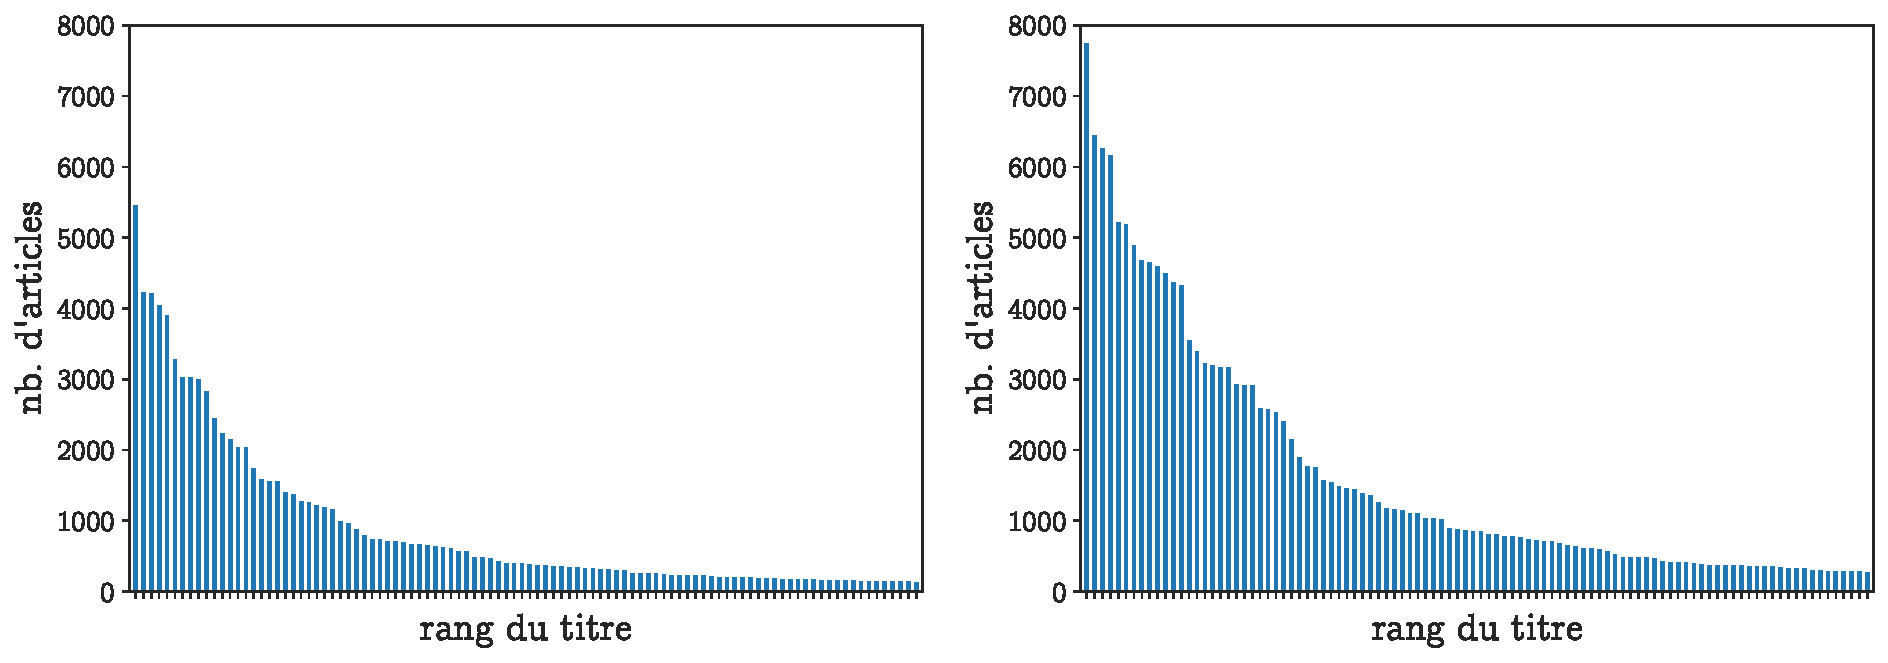
\includegraphics[width=\textwidth]{images/title_normalisation.pdf}
\caption{La fréquence des 100 titres les plus courants avant la normalisation (à gauche) et après}
\label{fig:title_normalisation}
\end{figure}




\subsection{Exploration} \label{exploration}

Cette section présente un aperçu général du corpus et ses tendances quantitatives, mais jette également un regard sur le contenu des articles et démontre les sujets principaux abordés au cours du siècle. Les manipulations contenues dans cette section se trouvent dans le \textit{notebook} correspondant.\footnote{\texttt{./notebooks/corpus\_exploration.ipynb}}

\subsubsection{Tendances de la quantité et la répartition de l'information} \label{corpus_tendencies}

La quantité de l'information dans le journal n'est pas répartie de façon homogène. Au cours de 86 ans\footnote{cf. la note en bas de la page \pageref{86_years}}, il y a des changements par rapport à la fréquence de parution, ainsi bien que une tendance à l'allongement des articles et l'augmentation de la masse d'information. Ces évolutions sont présentées sur la figure \ref{fig:text_mass}. Tout d'abord, l'on remarque que la fréquence de parution est divisée en trois étapes (en haut à gauche de la figure). Dans la première étape, avant 1830, \textit{Rigasche Zeitung} était publié ca. 100 fois par an, soit chaque mercredi et samedi. En 1828-1829, les jours de publication étaient le mardi, le jeudi et le samedi. Enfin, à partir de la fin de 1843, \textit{Rigasche Zeitung} est devenu un quotidien publié 6 fois par semaine, soit tous les jours sauf le dimanche. En haut à droite de la figure, le nombre moyen d'articles inclus dans un numéro est présenté. L'on y voit une croissance générale qui est pourtant interrompue par des périodes de recul ou les numéros ont contenu moins d'articles en moyenne.

Le graphique en bas de la figure \ref{fig:text_mass} décrit la longueur textuelle des numéros (en nombre de caractères). Pour chaque décennie, une \og boite à moustaches \fg{} est présentée. Dans chaque boîte, la ligne orange marque la médiane pour la décennie donnée - cela signifie qu'une moitié des articles ont une longueur supérieure à cette valeur. Le bord supérieur de la boîte marque la longueur qui est supérieur à celle de 75\% des données. De la même manière, 25\% des textes sont plus courtes au bord inférieur de la boîte. Les petites lignes horizontales marquent les minima et maxima des données pour la décennie. Les points qui restent au-delà de ces lignes sont les valeurs aberrantes, c'est-à-dire les articles exceptionnellement courts ou longs dans le contexte de la décennie.

\begin{figure}[h]
\centering
\captionsetup{justification=centering}
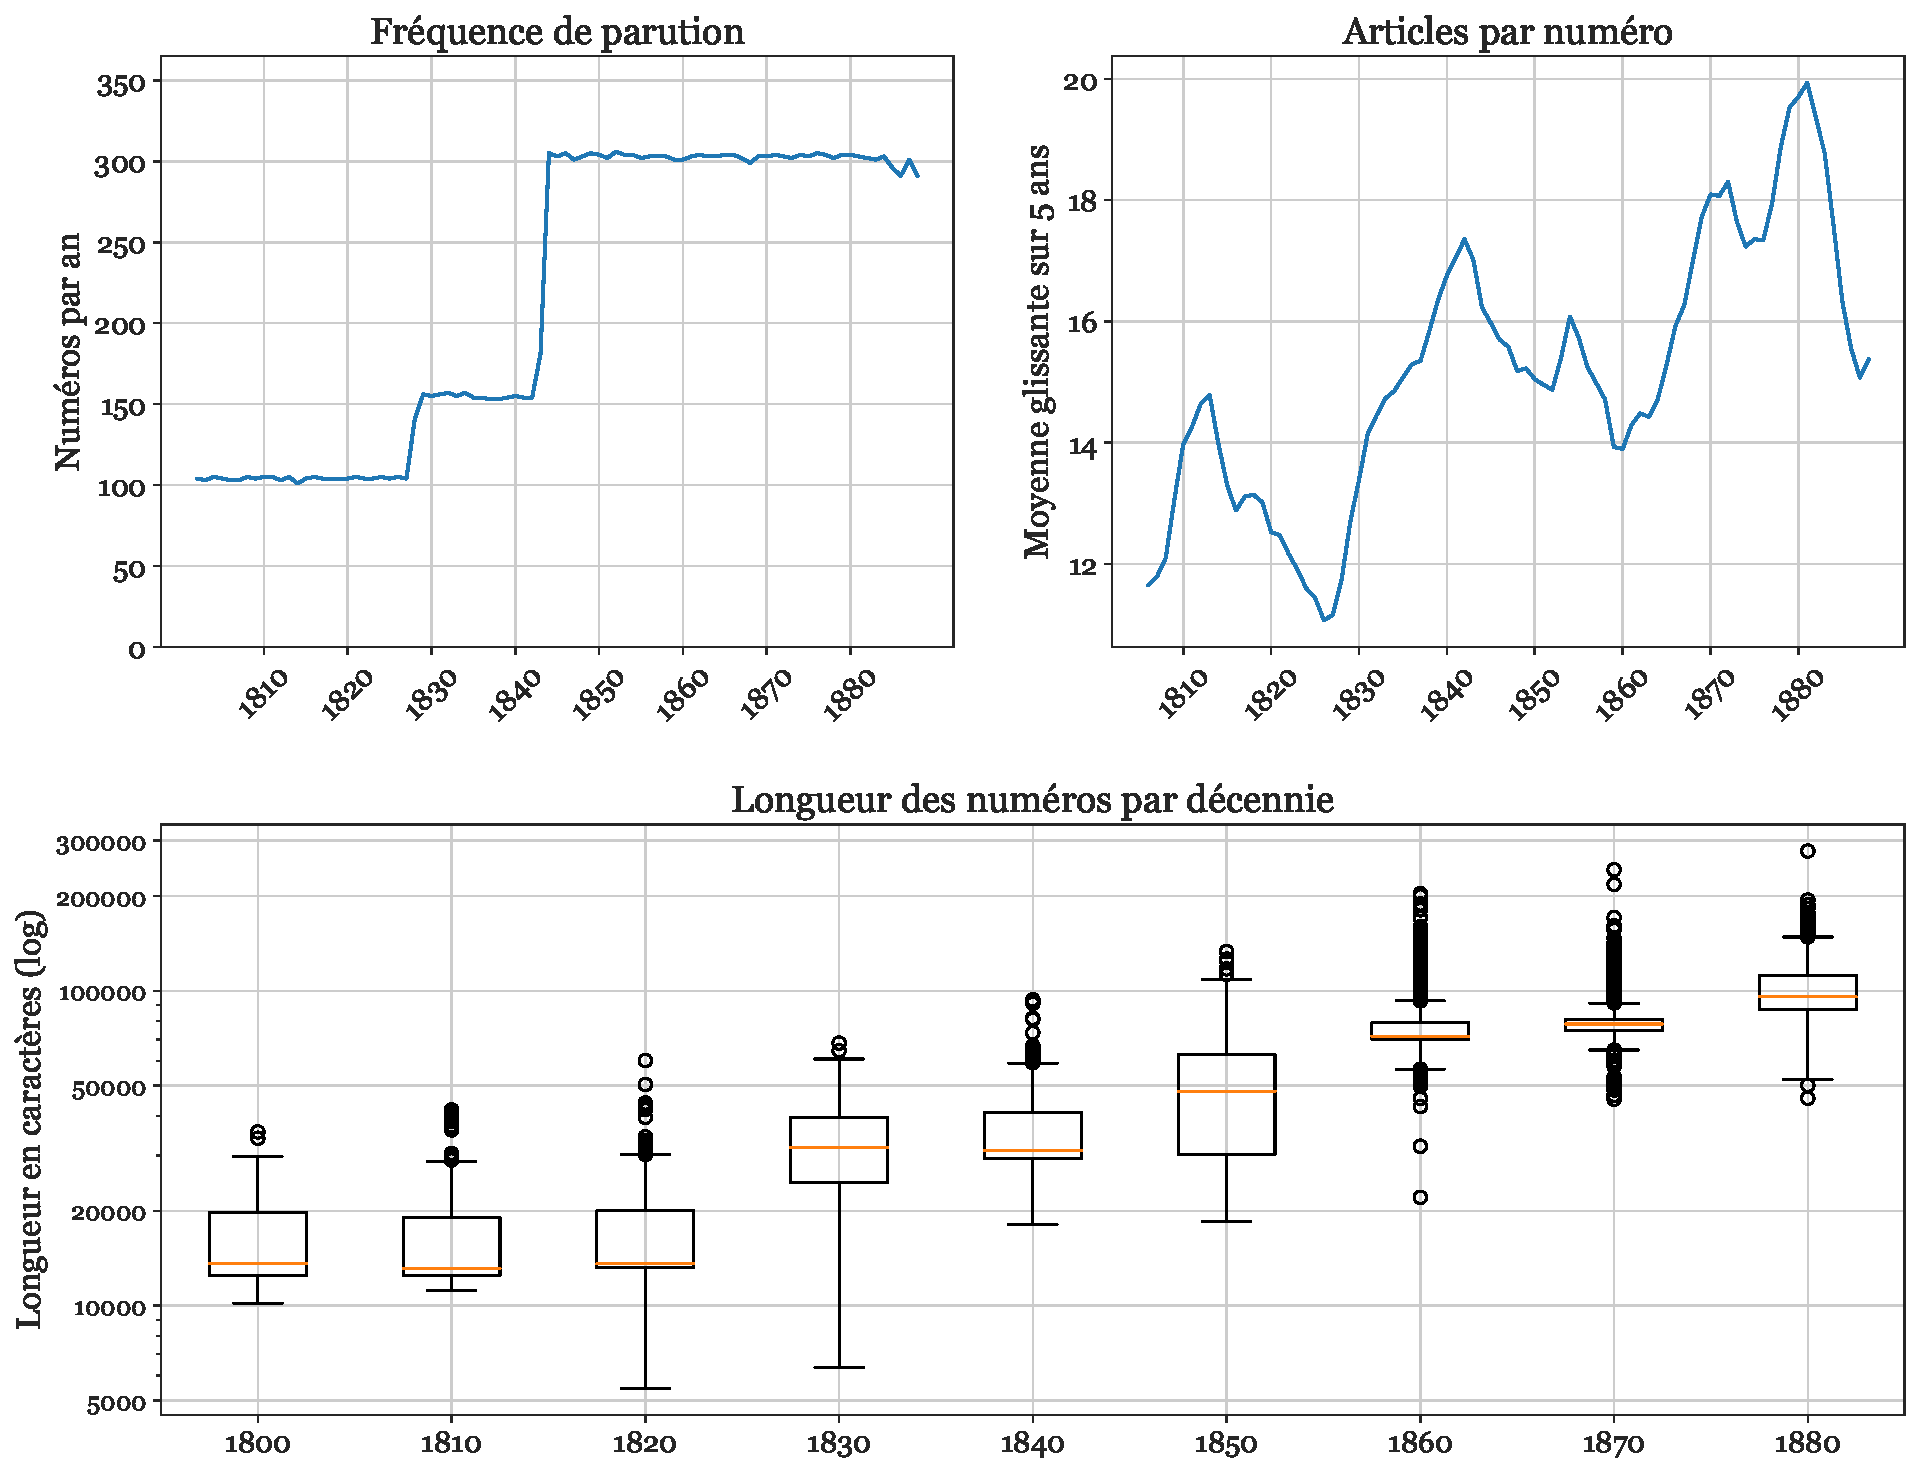
\includegraphics[width=\textwidth]{images/text_mass.pdf}
\caption{Evolutions par rapport à la quantité et la répartition temporelle de l'information}
\label{fig:text_mass}
\end{figure}

\clearpage

A l'aide des boîtes à moustaches, on perçoit que les numéros sont devenus plus longs au cours de la siècle. Jusqu'aux années 1830, le nombre de caractères dans un numéro restait normalement compris entre 10 000 et 30 000 (le minimum passant à 5000 dans les années 1820). Dans les années 1830-1850, la plupart des numéros étaient plus longs qu'auparavant, la médiane s'élevant à 50 000 caractères en 1850-1859. Les trois dernières décennies voient une configuration différente : les numéros deviennent plus longs avec une médiane finale de ca. 100 000 caractères en 1880-1888, mais il y a un nombre beaucoup plus élevé de valeurs aberrantes.\footnote{Il faut noter que l'axe vertical du graphique est sur une échelle logarithmique, ce qui donne une fausse impression que la distribution de la longueur des numéros est devenue plus étroite.}

En regardant les numéros avec une longueur disproportionnée, il dévient évident qu'à partir des années 1860, des annexes et des suppléments étaient souvent publiés en pièce jointe du numéro. La nature de ces types de textes était variée - des longues listes officielles des promotions des fonctionnaires à collections d'histoires littéraires, en passant par des informations sur les affaires judiciaires. La plupart du temps, le contenu de ces suppléments n'est pas strictement journalistique, mais ils ont quand même été numérisés par LNB comme parties des journaux, parfois portant leur longueur jusqu'à 40-50 pages.


\subsubsection{Contenu} \label{contenu}

Le journal change également dans le sens de son contenu. Ces dynamiques peuvent être perçues par les titres des articles et leur évolution dans le temps. Le tableau \ref{tab:common_headings} présente les 30 titres les plus fréquents dans le corpus entier, qui comptent pour ca. 40\% de tous les textes.\footnote{Les 10 titres les plus fréquents comptent pour 20\% et les 100 titres les plus fréquents pour 57\% du corpus} On voit que ces titres se répartissent en quelques catégories principales. Les articles portant le nom de l'origine de ses contenus sont très fréquents.\footnote{cf. la section \ref{pretraitement} pour les modifications qui facilitent le traitement des toponymes dans les titres} Les plus populaires parmi eux sont Paris, Londres, Vienne, Berlin, la France, l'Allemagne, St. Petersbourg, etc. - autrement dit les centres du pouvoir économique et politique dans l'Europe du XIX\textsuperscript{e} siècle qui canalisaient une grande proportion des informations importantes pour les lecteurs à Riga. Le public s'intéressait aux développements publics dans les grandes capitales (surtout en temps de guerre), ainsi qu'aux actualités coloniales qui se concentraient dans les métropoles. Les marchands suivaient des développements commerciaux qui avaient un effet sur leur métier. Le seconde type d'articles et celui des informations récurrentes, par exemple des listes d'étrangers arrivés ou partis par voie maritime ou terrestre, des télégrammes, les horaires de trains ou des rapport systématiques sur les commerce et la bourse.

\begin{table}[h]
    \centering
    \small
    \begin{tabular}{llr}
\toprule
                 \textbf{Titre} &         \textbf{Traduction française} & \textbf{Nb.} \\
\midrule
                          Paris &                                 Paris &      7771 \\
            Neueste Nachrichten &                   Dernières nouvelles &      6473 \\
                           Riga &                                  Riga &      6287 \\
                         London &                                Londres &      6192 \\
Witterungsbeobachtungen in Riga &   Observations météorologiques à Riga &      5242 \\
                           Wien &                                Vienne &      5216 \\
               Bekanntmachungen &                              Annonces &      4911 \\
                         Berlin &                                Berlin &      4684 \\
                     Frankreich &                                France &      4616 \\
             Angekommene Fremde &                     Etrangers arrivés &      4527 \\
        Inländische Nachrichten &                 Nouvelles domestiques &      4388 \\
                    Deutschland &                             Allemagne &      4350 \\
                 St. Petersburg &                       St. Petersbourg &      3642 \\
                     Telegramme &                           Télégrammes &      3571 \\
                         Inland &                [Affaires] domestiques &      3426 \\
                        Italien &                                Italie &      3246 \\
                         Inhalt &                   Contenu [du numéro] &      3217 \\
                    Vermischtes &                   [Actualités] mixtes &      3195 \\
     Groszbritannien und Irland &            Grande-Bretagne et Irlande &      3190 \\
         Tägliche Eisenbahnzüge &                     Trains quotidiens &      2958 \\
                         Madrid &                                Madrid &      2945 \\
                        Locales &                     [Affaires] locaux &      2939 \\
      Ist zu drucken erlaubt... &                Autorisé à imprimer... &      2621 \\
                    Oesterreich &                              Autriche &      2603 \\
                Deutsches Reich &                       Empire allemand &      2560 \\
Börsen- und Handels-Nachrichten & Actualités boursières et commerciales &      2435 \\
                 Konstantinopel &                        Constantinople &      2171 \\
                        Brüssel &                             Bruxelles &      1928 \\
                        England &                            Angleterre &      1802 \\
   Telegraphische Coursberichte &      Rapports de cours télégraphiques &      1788 \\
\bottomrule
\end{tabular}
    \caption{Les titres les plus courants dans le corpus}
    \label{tab:common_headings}
\end{table}

Bien entendu, ces catégories ne restent pas inchangées dans le temps. La partie suivante explore les développements principaux sur le contenu des journaux à l'aide des titres. Les titres ne reflètent pas complètement le contenu de l'article et ils ne sont pas toujours exacts (à cause d'une mauvaise segmentation, par exemple), mais ils sont pourtant adaptés pour donner une vue globale des sujets traités dans le journal.

Dans un premier temps, on peut regarder les lieux de provenance de l'information. La figure \ref{fig:headings_places} présente la part de l'importance des 10 noms de lieux étrangers les plus répandus dans le tableau \ref{tab:common_headings}, ainsi que les titres \textit{Inland}, \textit{Inländische Nachrichten}, \textit{Locales} et \textit{Riga}. Cette figure présente les titres de manière relative, ce qui signifie que la hauteur du graphique n'indique pas une valeur absolue, mais plutôt le pourcentage de tous les articles d'une année donnée.

\begin{figure}[h]
\centering
\captionsetup{justification=centering}
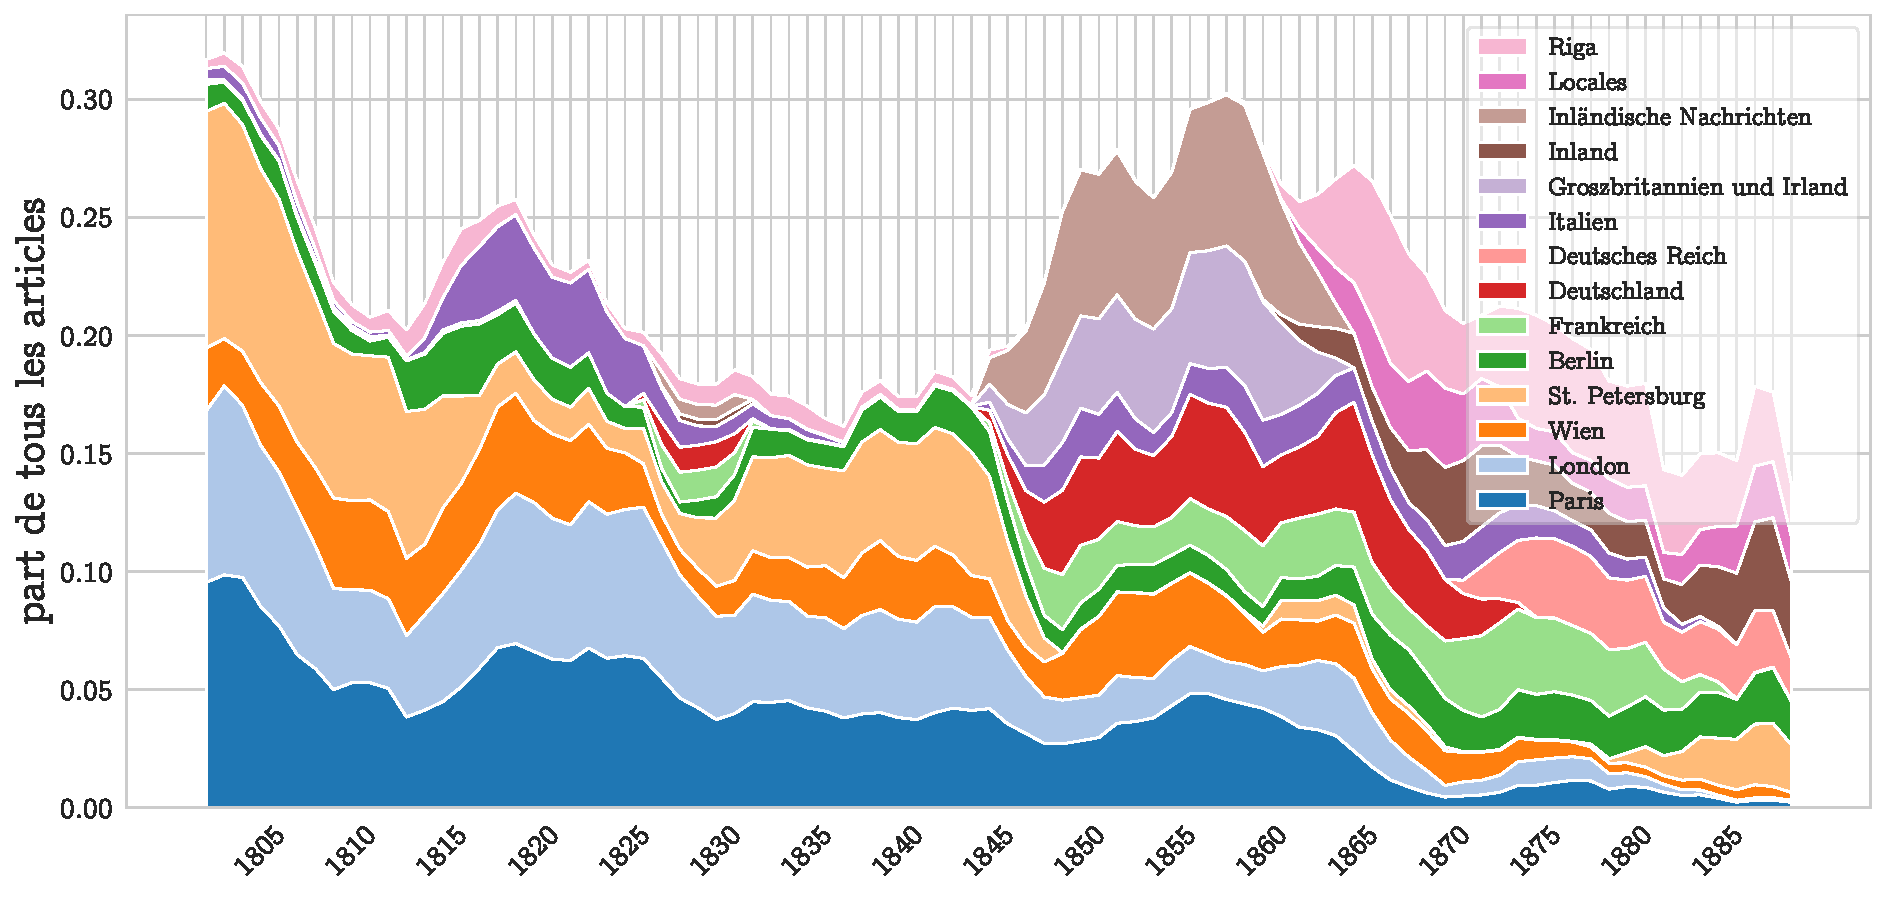
\includegraphics[width=\textwidth]{images/headings_places.pdf}
\caption{Importance relative des noms de lieux principaux dans les titres d'articles (moyenne glissante sur 5 ans)}
\label{fig:headings_places}
\end{figure}

On constate qu'au début de la période observée, les trois villes les plus importants paraissaient dans presque un tiers des titres, tandis que leur importance est tombée à moins de 5\% en 1888. D'une part, les titres ne reflètent pas toujours fidèlement le contenu des articles - les changements dans la structure des journaux, les décisions prises par LNB au stade de la segmentation, ainsi que un certain nombre des titres qui n'ont pas été capturés par l'expression régulière, influencent les proportions observées sur le graphique. Au fil du temps, différentes nouvelles de villes étrangères pourraient, par exemple, être progressivement incluses dans des articles aux noms plus généraux, déplaçant ainsi les noms de lieux au sein de l'article.

D'autre part, ces tendances reflètent probablement des vraies évolutions par rapport au contenu du journal. Au fur et à mesure que le réseau de journaux s'imbrique au cours du siècle et que la vitesse de l'information augmente, les journaux s'adaptent aux changements. Il est clair que le nombre de sources disponibles et accessibles était beaucoup plus petit au début du siècle qu'à la fin. La nature de ce que l'on considérait \og médiatique \fg{} a également changé. Dans les premières décennies du XIX\textsuperscript{e} siècle, les nouvelles dignes d'intérêt concernent des événements survenus à l'étranger, s'inscrivant ainsi dans la logique de la presse des débuts de l'ère moderne. Les informations locales étaient principalement transmises par d'autres moyens (par le bouche à oreille, affiches, etc.). Toutefois, au milieu du siècle, on constate un changement de tendance. Des nouvelles catégories importantes, d'abord \textit{Inland}/\textit{Inländische Nachrichten}, ensuite \textit{Locales} et \textit{Riga}, apparaissent. Cela représente un \og retour sur soi \fg{} très intéressant qui apparaît également dans d'autres journaux locaux de l'époque.\footnote{De 1836 à 1863, le journal \textit{Inland} était publié à Tartu (\textit{Dorpat}). Ce journal a été le premier dans les gouvernements baltes à s'éloigner de la vision des nouvelles comme quelque chose qui vient toujours de l'étranger. Il est possible que l'apparition de \textit{Inländische Nachrichten} dans le \textit{Rigasche Zeitung} dans le même temps est une réponse à cela.} Dans \textit{Rigasche Zeitung}, la catégorie \textit{Inland} représente en fait l'ensemble de l'empire russe avec un accent sur les villes des gouvernements Baltes et apparaît au moment où la fréquence de parution atteint 6 jours par semaine. La catégorie \textit{Locales} se concentre principalement sur les événements au niveau de Riga ou ses alentours.

Une autre évolution très intéressante, ou plutôt une rupture, peut être observée lorsque nous examinons les titres du tableau \ref{tab:common_headings} qui expriment quelque chose sur la forme ou le mouvement de l'information. En regardant les titres sélectionnés pour la figure \ref{fig:headings_other}, on remarque tout de suite la rupture vers l'année 1860. En fait, ce graphique, ainsi que le précédent, ont été crées avec une moyenne glissante sur 5 ans pour niveler un peu les tendances et pour les rendre plus faciles à percevoir. En retirant la moyenne glissante, cette rupture est encore beaucoup plus subite - tous les titres concernés tombent à zéro en 1855 et ne remontent qu'en 1861. Cela correspond à peu près à la période de la guerre de Crimée (1853-1856), pendant laquelle les ports russes étaient bloqués par les marines de la France et le Royaume-Uni. En situation de guerre, la presse avait sa propre sorte de \og silence radio \fg{}, au moins en ce qui concerne ces importantes catégories d'articles, car la masse totale d'articles et de l'information n'est pas considérablement influencée.

\begin{figure}[h]
\centering
\captionsetup{justification=centering}
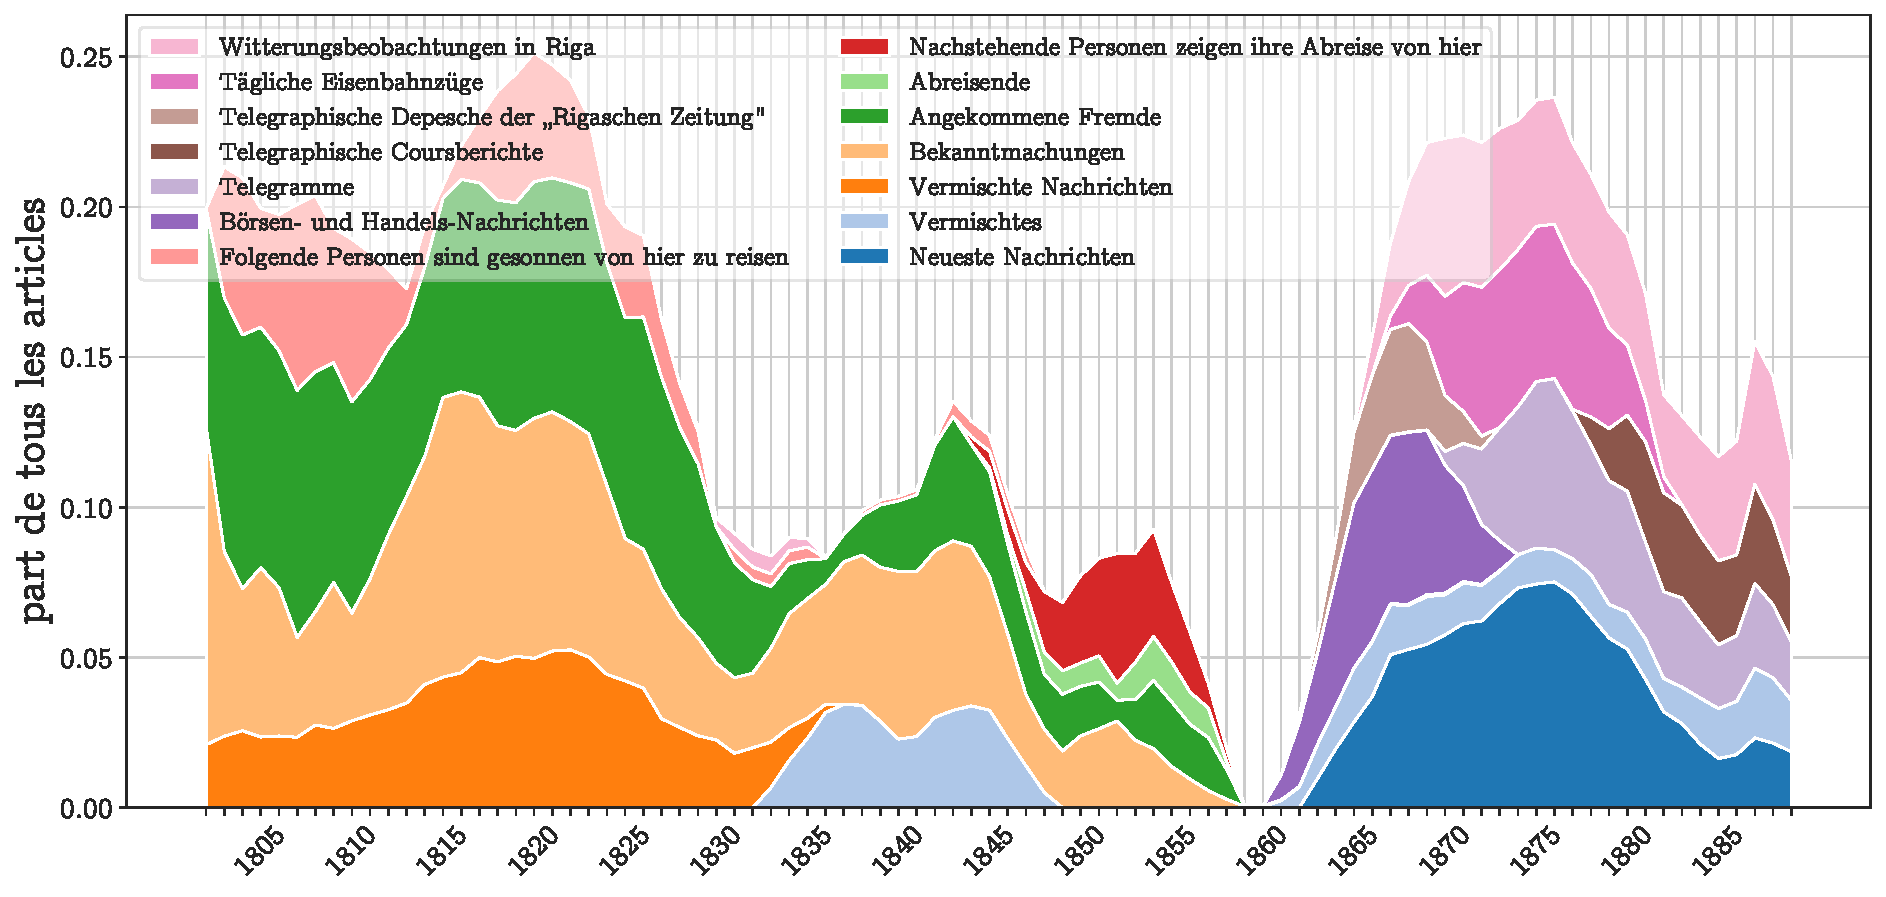
\includegraphics[width=\textwidth]{images/headings_other.pdf}
\caption{Importance relative des titres donnés (moyenne glissante sur 5 ans)}
\label{fig:headings_other}
\end{figure}

Les années 1855-1860 marquent un changement brusque pour le \textit{Rigasche Zeitung} dans la mesure où le journal qui a émergé après cette période était très différent de celui qui l'avait précédé. Les vieilles catégories d'information qui étaient importantes auparavant, notamment les étrangers arrivés, les départs et les annonces, disparaissent complètement. A leur place, une multitude de rubriques inédites font surface : télégrammes. actualités boursières, horaires des trains etc. Prises ensemble, ces nouvelles catégories d'information qui ont rapidement constitué une part considérable du numéro moyen, peuvent être considérées collectivement comme un signe de l'avènement de la modernité.

En novembre 1852, une des premières lignes télégraphiques publiques en Europe du Nord et la première ligne électromagnétique dans l'Empire russe a été ouverte entre Riga et Bolderāja (\textit{Bolderaa}), où le fleuve Daugava (\textit{Düna}) atteint la mer Baltique, à environ 10 km du centre de Riga.\footcite[48-54]{petersone_rigas-bolderajas_1999} Le télégraphe y fût installé principalement pour avertir les marchands de Riga sur les conditions météorologiques et maritimes en temps réel, ce qui était considéré comme crucial pour la navigation.\footnote{Les soucis des marchands étaient exprimés aussi dans la presse. Par exemple, le journal \textit{Das Inland} (cf. la page \pageref{das_inland}) écrit en 1836 : \og Comme il est probable que la communication avec la Bolderaa sera bientôt et peut-être déjà fermée, nous n'en apprendrons naturellement rien, sinon ce que les personnes qui montent dans nos clochers, souvent armées de jumelles, jugeront bon de nous communiquer. C'est pourquoi nous ne pouvons pas assez répéter le souhait que des dispositions soient prises pour que nous soyons sûrs et rapides soient informées de ce qui s'y passe et de l'intérêt qu'elles suscitent. un intérêt si général. \fg{} \textit{Das Inland}, 20.04.1836} 

Trois ans plus tard, une autre ligne télégraphique a été ouverte de Riga à Daugavpils, une ville située au sud-est des Gouvernements baltes. En 1857, Riga a obtenu deux autres lignes télégraphiques : une vers Tallinn, la capitale du gouvernement d'Estonie, qui était à son tour reliée à Saint-Pétersbourg ; et une autre vers la frontière prussienne. Ces lignes ont effectivement relié Riga au réseau télégraphique européen.\footcite[151]{petersone_vidzemes_1998} À la même époque, en septembre 1861, Riga a eu sa première liaison ferroviaire avec la ville de Daugavpils, qui était à son tour reliée à Saint-Pétersbourg, Vilnius et Varsovie. Cela a également entraîné des changements dans le système postal, car le courrier a commencé à être acheminé par voie ferroviaire.\footcite[153]{petersone_vidzemes_1998}

Ces développements sont bien reflétés dans la structure de \textit{Rigasche Zeitung} à partir des années 1860. On voit la disparition complète de la rubrique des passagers arrivés - autrefois une source principale pour toute personne qui voulait recevoir des nouvelles directes des provinces de l'empire ou d'autres villes d'Europe. L'avènement des nouvelles voies de communication a rendu caduque les anciens modes de pensée et a inséré le journal dans un réseau moderne d'information en expansion constante, constitué de chemins de fer, de lignes télégraphiques et, au XX\textsuperscript{e} siècle, de téléphones. Les informations sur les cours de la bourse dans des villes éloignées pouvaient être communiquées en quelques minutes et les trains ont érodé l'attrait du voyageur lointain. Au lieu de regrouper les nouvelles redondantes ou moins importantes sous la rubrique \og nouvelles mixtes \fg{} (\textit{Vermischtes}), le journal a commencé à les présenter comme les \og dernières nouvelles \fg{} - ici aussi, la rapidité et la fraîcheur ont de la valeur.

\label{beobachtungen_riga}Il faut aussi s'arrêter sur la rubrique des observations météorologiques qui sont parmi les catégories de nouvelles les plus nombreuses. Un peu à l'inverse de ce à quoi le lecteur moderne est habitué, il ne s'agissait pas de prédictions météorologiques, mais de rapports sur le temps du ou des jours précédents. Avec quelques changements au fil du temps, ils se composaient normalement de quelques mots-clés (exprimant les précipitations et la vitesse du vent) et de mesures numériques (sur la température et la pression atmosphérique) disposés dans une sorte de tableau. Malheureusement, c'est ce type de présentation qui rend les observations météorologiques inutilisables dans le contexte du présent travail, car l'OCR est souvent de très mauvaise qualité sur ces articles (voir le tableau \ref{tab:readability_example} pour un exemple). Seuls 45 (!) des 5194 articles de cette catégorie ont été considérés comme lisibles par le modèle SVM. Les exclure des prochaines étapes de l'analyse signifie beaucoup de potentiel inutilisé, mais aussi un objectif plus clair - ils diffèrent très clairement du type descriptif d'informations météorologiques que l'on trouve normalement dans d'autres types d'articles. Les observations météorologiques peuvent encore témoigner de l'intérêt croissant pour le temps et d'une approche empirique renouvelée dans les dernières décennies du siècle, ce qui peut également être utile pour comprendre les textes de type narratif.


\clearpage




\section{Mentions du temps}\label{mentions_du_temps}

Ce chapitre porte sur le contenu \og climatique \fg{} au niveau des mots isolés qui signifient des phénomènes météorologiques en allemand et leur présence dans le corpus. Tout d'abord, le corpus sera vectorisé. Les vecteurs de mots, également appelés \textit{word embeddings}, contiennent des informations sur les contextes dans lesquels les mots apparaissent et peuvent être utilisés pour effectuer différents types d'analyses, notamment des comparaisons sémantiques. Ensuite, un vocabulaire fixe des mots \og météorologiques \fg{} sera construit. Les occurrences de chaque mot-clé seront comptées afin de voir leur distribution et d'effectuer des analyses comparatives ainsi que temporelles. La vectorisation des textes offre également la possibilité de visualiser les relations sémantiques entre des mots. Enfin, les contextes immédiats des mots-clés seront étudiés. Les analyses de ce chapitre restent donc au niveau des mots individuels et leurs contextes proches, mais peuvent être mises dans le contexte des tendances générales exposées dans le chapitre précédent et forment une base pour les analyse de sujets dans la partie suivante.

La partie actuelle du travail part de la notion simple que les textes dans le corpus qui contiennent de l'information sur le climat et le temps sont reconnaissables par la présence de certains mots-clés. Le défi principal de cette approche se présente sous la forme du bruit dans le corpus : une liste des mots pertinents ne compterait jamais toutes les formes orthographiques qui apparaissent dans l'intégralité d'articles.

\subsection{Tentative par une approche à base des entités nommées}\label{NER_approach}

Une prémière tentative de contourner ce problème de variance textuelle a été faite avec les méthodes de la reconnaissance d'entités nommées (NER). Selon D. Jurafsky et J. Martin, 

\begin{displayquote} \textit{Une entité nommée est en gros, tout ce qui peut être désigné par un nom propre : une personne, un lieu, une organisation. La tâche de la reconnaissance des entités nommées (NER) consiste à trouver des parties de texte qui constituent des noms propres et à marquer le type d'entité. Quatre balises d'entité sont les plus courantes : PER (personne), LOC (lieu), ORG (organisation) ou GPE (entité géopolitique). Cependant, le terme entité nommée est généralement étendu pour inclure des choses qui ne sont pas des entités en soi, notamment des dates, des heures et d'autres types d'expressions temporelles, et même des expressions numériques comme les prix.}
\footcite[153]{jurafsky_speech_2020}\end{displayquote}

\label{NER_model}
L'idée d'une approche des descriptions climatiques et météorologiques via des entités nommées reposait donc sur le fait de considérer tous les mots-clés pertinents comme appartenant à une catégorie distincte d'entités qui peuvent ensuite être détectées par un modèle de langage. Comme un tel modèle ne repose pas sur une liste fixe des formes orthographiques mais prend en compte un nombre des paramètres cachées dans le contexte, il pourrait théoriquement détecter des mots non vus précédemment. Un modèle supervisé de la reconnaissance des entités nommées a donc été entraîné : toutes les entités dans une échantillon ont été annotées manuellement pour apprendre à l'ordinateur à reproduire cette logique sur le reste du corpus. L'échantillon comprenait 400 textes et a été annoté avec la schéma suivante :

\vspace{1ex}
\begin{itemize}[label=$\bullet$]
    \item \texttt{WEA} - phénomènes météorologiques exprimées par des substantifs ou des groupes nominaux, ainsi que quelques mots plus généraux liés au climat (853 instances dans l'échantillon) 
    \item \texttt{LOC} - lieux (2939 instances)
    \item \texttt{DAT} - dates (1035 instances)
    \item \texttt{PER} - noms de personnes (1320 instances)
\end{itemize}
\vspace{2ex}

La schéma reflète aussi les buts initiaux de la recherche qui visaient une détection, datation et géolocalisation des événements climatiques. En se basant sur la structuration d'information dans le journal, l'hypothèse était que l'occurrence d'un mot clé est souvent accompagnée par une date et le lieu. La quatrième catégorie, \texttt{PER}, était ajoutée à la schéma pour éviter la confusion entre les toponymes et les noms de personnes (par exemple les noms des nobles sont souvent les lieux de leur provenance), ainsi qu'entre les phénomènes climatiques et les noms de personnes (certains mots comme \textit{Sturm} apparaissent parfois comme des noms de famille en allemand).

Toutefois, la performance du modèle de reconnaissance des entités nommés formé sur ces données était trop faible pour effectuer des analyses significatives. La précision (combien des occurrences trouvées sont correctes), ainsi que le rappel (combien des occurrences totales ont été détectés) étaient médiocres, un fait lié surtout au bruit introduit au stade de l'océrisation, mais aussi aux particularités d'un texte historique qui peuvent confondre un modèle dont le fond a été créé sur des données contemporaines. La prémisse théorique de considérer les événements climatiques comme des entités nommées peut également avoir ses limites car strictement, il ne s'agit des noms propres.

Ces circonstances n'offraient pas trop de choix pour une amélioration du modèle. Une possibilité aurait été d'adapter le modèle de langue au corpus et à la langue historique qui, à son tour, aurait nécessité un travail très ardu et technique, sans garantir de meilleurs résultats. La deuxième option, la plus évidente, aurait été l'augmentation des données d'entraînement. Cela, toutefois, ne montraient pas de signes prometteurs d'amélioration, par exemple entre des échantillons de 300 et de 400 textes. Le temps nécessaire pour l'annotation et le double contrôle aurait était si long qu'il paraissait mieux de s'appuyer sur une simple distribution des mots.


\subsection{Une approche en sémantique distributionnelle} \label{distributional_semantics_approach}

L'échec d'une approche supervisée m'a amené à une approche par un ensemble fixe de mots \og climatiques \fg{}. Afin de contourner le problème du bruit décrit ci-dessus, j'ai opté pour une solution qui s'appuie sur la similarité vectorielle entre les formes \og propres \fg{} et les formes alternatives. L'idée de la sémantique vectorielle repose sur l'hypothèse de distribution développée dans les années 1950. Selon celle-ci, le plus que les significations d'un mot et l'autre sont similaires, le plus ils apparaissent dans un contexte similaire. Par exemple, les mots voisins de \textit{voiture} et \textit{automobile} sont très similaires. L'hypothèse de distribution dit alors que leurs significations devront être très similaires ou presque identiques, car ils sont interchangeables dans la plupart des cas.\footcite[96]{jurafsky_speech_2020} L'un des principaux avantages des vecteurs de mots est la possibilité de mesurer et de comparer la \og distance \fg{} entre deux mots. Un vecteur, qui est essentiellement une rangée de chiffres, peut être traité comme un point de coordonnées dans un espace hyperdimensionnel (le nombre de dimensions correspondant à la longueur du vecteur). Lorsque deux mots ont des contextes similaires, leurs encastrements résultants sont également similaires, ce qui signifie qu'ils sont également positionnés de manière proche dans l'espace hyperdimensionnel.

Il existent plusieurs méthodes pour calculer les vecteurs des mots. Dans le travail actuel, la méthode \textit{word2vec} est utilisée. Publiée par Tomas Mikolov et ses collègues en 2013,\footcite{mikolov_distributed_2013} \textit{word2vec} utilise la distribution des mots dans un corpus pour entraîner un classificateur pour la tâche \og est-il probable que le mot \textit{x} apparaisse près du mot \textit{y} ? \fg{}. Dans le cas de \textit{word2vec}, les prédictions elles-mêmes n'ont pas réellement de valeur. A leur place, les pondérations (\textit{weights}) du classificateur sont utilisées comme les vecteurs.\footnote{Les pondérations sont les paramètres que le modèle apprend à ajuster au cours de l'entraînement. Dans un réseaux de neurones, les pondérations sont en fait les multiplicateurs qui modifient les valeurs d'entrée à chaque couche du réseaux.} Cela veut dire que les chiffres ne sont pas d'une interprétation directe, mais ils définissent quand même la position des mots dans l'espace sémantique - ils ont une valeur relative. Une fois que les vecteurs sont calculées, des simples opérations mathématiques peuvent être appliquées pour calculer la distance entre eux, ce qui correspond à une similarité dans la signification selon l'hypothèse de distribution.\footcite[112-113]{jurafsky_speech_2020}

Pour calculer les vecteurs des mots du corpus LNB, les articles \textit{tokenisés}\footnote{\texttt{.data/processed/RZ\_tokenized.jsonl}} ont été parcourus par le modèle \textit{word2vec}.\footnote{\texttt{./climdist/train\_word2vec.py} - les paramètres pour l'entraînement étaient \texttt{vector\_size = 100} (les vecteurs ont une longueur de 100 nombres et se situent donc dans un espace de 100 dimensions), \texttt{min\_count = 10} (un mot doit apparaitre au moins 10 fois pour avoir une vecteur), \texttt{epochs = 10} (le corpus est itéré 10 fois au cours du calcul). Le modèle \textit{word2vec} se trouve dans \texttt{./data/processed/models/word2vec/}} Une démonstration générale du modèle \textit{word2vec} entraîné sur le corpus se trouve dans le tableau \ref{tab:similar_vectors}. Sous chaque mot d'entrée, les 10 mots les plus similaires à eux selon la distance vectorielle sont listés dans l'ordre de leur similarité. Parmi les mots similaires se trouvent des synonymes (\textit{rasch}, \textit{eilig}), des formes altérées (\textit{Krieges}, \textit{genommen}), des hyponymes (\textit{Bürgerkrieg}, \textit{Feldzug}, \textit{Nordamerika}), des concepts associés (\textit{Kampf}, \textit{Australien}), ainsi que des formes mal-orthographiées (\textit{nebmen}, \textit{uehmen}, \textit{rafch}, \textit{kamps}), mais aussi des antonymes (\textit{langsam}). Ces exemples sont suffisants pour démontrer que la distance vectorielle réussit à capturer des relations intuitives entre les mots, même dans le cas des erreurs orthographiques. Là aussi, c'est la taille du corpus qui permet d'obtenir des résultats solides, car les formes alternatives apparaissent un nombre suffisant de fois dans l'ensemble des textes.


\begin{table}[h]
    \centering
    \small
    \begin{tabular}{llll}
\toprule
            \textbf{amerika} &            \textbf{krieg} &         \textbf{schnell} &    \textbf{nehmen} \\
\midrule
        nordamerika &           kriege &           rasch &    nebmen \\
             canada &          krieges &       schneller &     nehme \\
bereinigten\_staaten &      bürgerkrieg &         langsam &  genommen \\
       nord-amerika &     bürgerkriege &         rascher &    uehmen \\
vereinigten\_staaten &     krieg\_führen &           rafch &    nähmen \\
         südamerika & feindseligkeiten &     unterdessen &     nimmt \\
         australien & ausbruch\_krieges &          kurzer &    nommen \\
        kalifornien &            kampf &           eilig &     ehmen \\
        süd-amerika &          feldzug &         alsbald &    nehwen \\
             kanada &            kamps & wenigen\_minuten & nehmenden \\
\bottomrule
\end{tabular}
    \caption{Les mots le plus similaires à \textit{Amérique}, \textit{guerre}, \textit{vite}, \textit{prendre}}
    \label{tab:similar_vectors}
\end{table}

Pour construire un vocabulaire fixe des mots liés au climat à l'aide de la similarité vectorielle, un ensemble de départ des mots-clés a été choisi pour y ajouter des formes alternatives, ainsi que des hyponymes et des synonymes.\footnote{Cet ensemble de départ se trouve dans \texttt{./pipeline/keyword\_patterns.json}} Le cœur du ce vocabulaire consiste en 42 mots signifiant des phénomènes climatiques, ainsi que des termes généraux comme le climat, le temps etc (voir le tableau \ref{tab:weather_events}). L'ensemble est limité aux noms - des verbes comme \textit{regnet} (il pleut) et des adjectifs comme \textit{regnerisch} (pluvieux) ne sont pas inclus pour garder la petite taille de l'ensemble et la cohésion des analyses. La grande majorité des mots signifient donc des événements météorologiques (à l'exception des mots \textit{Klima}, \textit{Wetter} et \textit{Witterung} qui sont des catégories plus générales), mais ils peuvent varier selon leur délimitation temporelle (par exemple \textit{Orkan} (ouragan) vs \textit{Dürre} (sécheresse)). En général, les 42 mots sont choisis pour représenter les catégories d'événements météorologiques qui existent dans la base de données Euro-Climhist.

\label{synonymes}Certains mots dans l'ensemble peuvent également avoir des significations ou un usage hors du climat et de la météorologie - plus notamment les mots \textit{Wärme} (chaleur) et \textit{Kälte} (froid). D'autres, avant tout le mot \textit{Sturm} (tempête), apparaissent souvent dans un sens métaphorique (par exemple une tempête (fureur) politique, une tempête des sentiments, etc.) ou font partie d'expressions idiomatiques (\textit{im Sturm nehmen} - prendre l’assaut, \textit{die Stille vor dem Sturm} - le calme avant la tempête, \textit{der Sturm im Wasserglas} - la tempête dans un verre d’eau, etc. etc.).

\begin{table}[h]
    \centering
    \small
\begin{tabular}{llll}
\toprule
      dürre & niederschlag &  schneefall &       westwind \\
       flut &  nordostwind &       sturm &         wetter \\
      frost & nordwestwind &   sturmwind &           wind \\
   gewitter &     nordwind &  südostwind &     windstärke \\
      hagel &        orkan & südwestwind &    wirbelsturm \\
hagelschlag &      ostwind &     südwind &     wirbelwind \\
      hitze &        regen &      taifun &      witterung \\
 hochwasser &    regenfall &   thauwetter &    wolkenbruch \\
      klima &     regenguß &        thau &          wärme \\
      kälte & regenschauer &     tornado & überschwemmung \\
      nebel &       schnee &    unwetter &            \\
\bottomrule
\end{tabular}
    \caption{L'ensemble de base des mots-clés}
    \label{tab:weather_events}
\end{table}

A partir de ces 42 mots, l'ensemble a été élargi à l'aide de la similarité vectorielle. Pour chaque mot dans la liste originelle, les 100 mots les plus proches ont été examinés pour en choisir ceux qui ont une signification similaire.\footnote{\texttt{./notebooks/keywords.ipynb}} Les mots qui expriment des événements ou des concepts climatiques mais qui n'étaient pas présents dans l'ensemble de base ont également été ajoutés. La sélection était toujours limitée aux noms, mais des bigrammes avec un composant adjéctif (\textit{bewölkter\_himmel}, ciel nuageux)  ou verbe (\textit{wind\_weht}, le vent souffle) ont été inclus.

Le vocabulaire final comprend alors \textbf{323} schémas différentes.\footnote{\texttt{./pipeline/keyword\_patterns.xlsx}, colonne \texttt{key}} Ensuite, toutes les formes trouvées ont été reliées à leurs formes propres afin de ne pas fragmenter les résultats de l'analyse dans les phases ultérieures (en séparant, par exemple, les distributions de \textit{Regen} et \textit{Regens}). Cette réduction ne concerne que les formes infléchies, mal orthographiés ou bruitées d'une même racine (par exemple \textit{wiud}, \textit{winde}, \textit{windes} sont regroupés sous la forme \og canonique \fg{} \textit{wind}). Le nombre total des formes propres est de \textbf{157}, qui peut donc être considéré la taille finale du vocabulaire.\footnote{\texttt{./pipeline/keyword\_patterns.xlsx}, colonne \texttt{wordform}}

Les vecteurs obtenus par \textit{word2vec} peuvent être utilisés pour visualiser les relations sémantiques entre les mots-clés en tant qu'ils apparaissent dans le corpus. Les expériences ont montré que, parmi les différentes méthodes de réduction de dimension, UMAP\footcite{mcinnes_umap_2020} est la meilleure solution pour projeter les vecteurs à 100 dimensions dans un espace à deux dimensions, car elle conserve à la fois les distances locales et globales. Afin de privilégier l'interprétabilité à la quantité, les formes normalisées des mots-clés ont été utilisées pour le mappage. Comme les formes brutes des mots qui existent dans le corpus sont beaucoup plus diverses et ont des vecteurs légèrement différents des formes propres, la moyenne vectorielle de toutes ses formes brutes a été utilisée pour représenter chaque mot normalisé. La figure \ref{fig:keyword_umap} présente donc les distances vectorielles entre tous les mots-clés sous ses formes propres, i.e. normalisées.\footnote{Les calculs se trouvent dans \texttt{./notebooks/word\_vectors.ipynb}}

\begin{figure}[h]
    \centering
    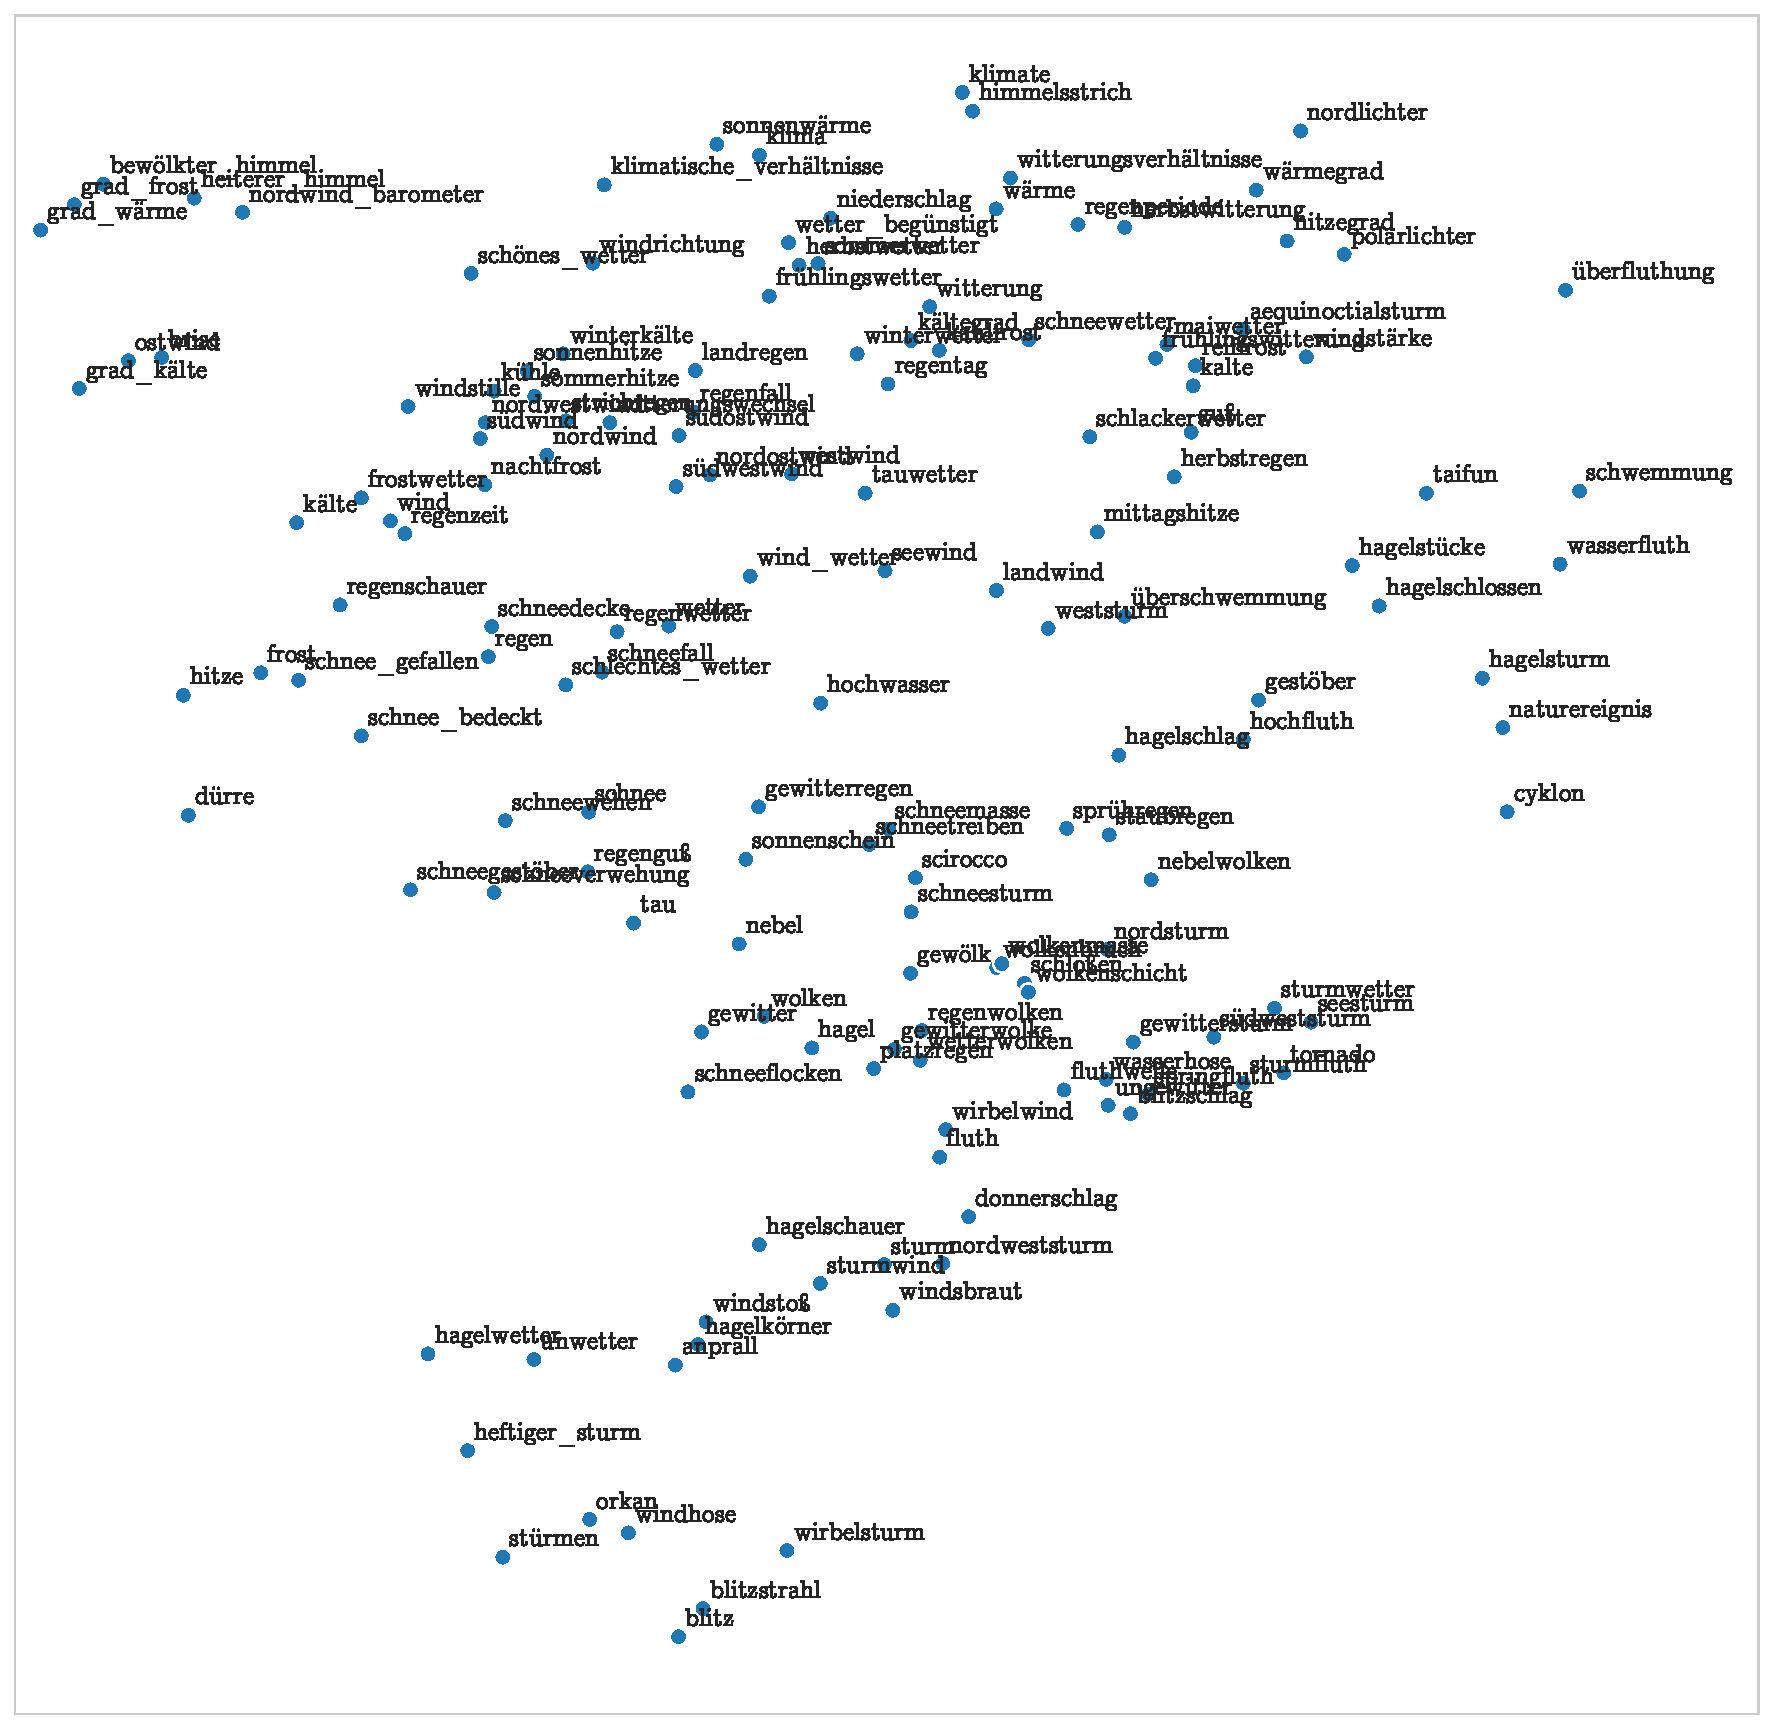
\includegraphics[width=0.9\textwidth]{images/keyword_umap.pdf}
    \caption{Une visualisation spatiale des vecteurs de mots-clés}
    \label{fig:keyword_umap}
\end{figure}

On constate que les mots-clés sont regroupés assez intuitivement. Par exemple, la plupart des mots liés à la neige (\textit{schnee}, \textit{schneegestöber}, \textit{schnee\_bedeckt}, \textit{schnee\_gefallen}, etc.) se concentrent autour de la partie gauche du graphique. En haut se trouvent les mots pour le climat et le temps (\textit{klimate}, \textit{klimatische\_verhältnisse}, \textit{witterung}, \textit{frühlignswetter}, etc.). Les concepts liés à la tempête forment un nuage flou autour de la partie inférieure centrale (\textit{wirbelwind}, \textit{nordweststurm}, \textit{tornado}, \textit{sturmwetter}, etc.), pendant que leurs variations plus extrêmes se concentrent en bas du graphique (\textit{heftiger\_sturm}, \textit{orkan}, \textit{wirbelsturm}, \textit{unwetter}). Il existent aussi des conceptes qui se répartissent de manière assez homogène dans le graphique, notamment les mots liés à la pluie et à la grêle. Il faut garder à l'esprit que les vecteurs de \textit{doc2vec} ne représentent les relations sémantiques dans aucune façon absolue ; au sens strict, la proximité des deux vecteurs dans le graphique est l'expression de la similarité de leurs contextes dans le corpus. L'omniprésence relative de la pluie et la grêle est donc un signe que ces mots apparaissent dans des contextes plus divers. En revanche, les mots dans la partie supérieure gauche (\textit{bewölkter\_himmel}, \textit{grad\_wärme}, \textit{grad\_frost}, \textit{nordwind\_barometer}) sont ceux qui sont très souvent utilisés dans le style répétitif des observations météorologiques.

En général, les interrelations entre les mots-clés se conforment plus ou moins à une compréhension moderne et quotidienne de la terminologie météorologique (à quelques exceptions près, par exemple le mot mot archaïque pour la tempête, \textit{Windsbraut}). Le vocabulaire créé à l'aide des distances vectorielles et les positionnements des mots dans l'espace vectorielle montrent que les mots liés au climat étaient perçus de façon relativement similaire à celle d'aujourd'hui. 


\subsection{Distribution et tendances des mots-clés météorologiques}\label{entity_distribution}

\begin{wrapfigure}{r}{0.48\textwidth}
  \begin{center}
    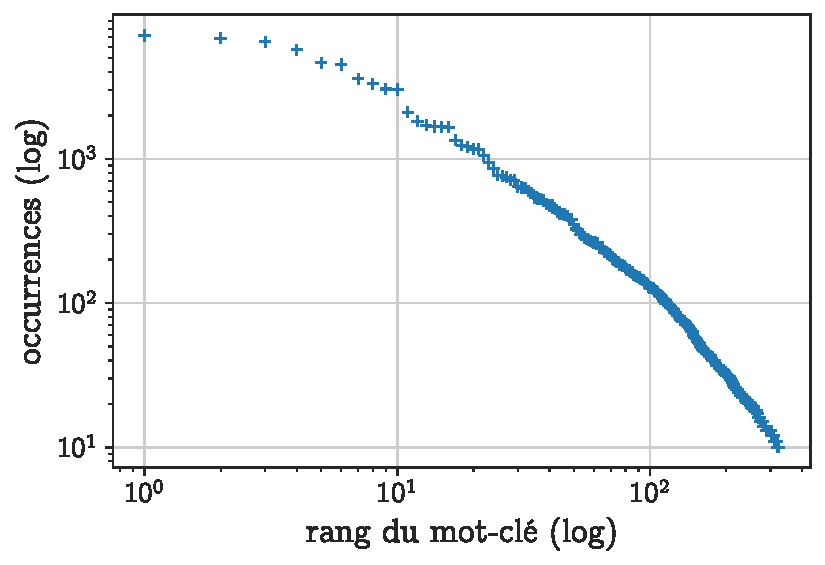
\includegraphics[width=0.48\textwidth]{images/zipf.pdf}
  \end{center}
  \vspace*{-2ex}
  \captionsetup{justification=centering}
  \caption{Nombre des mots-clés par rang sous ses formes originelles}
  \label{fig:zipf}
\end{wrapfigure}

% >>> pretraitement
% Pour les analyses suivantes, seules les entités qui se trouvent dans les articles \og lisibles \fg{} sont prises en compte pour garder une continuité numérique à travers les différentes étapes du travail.

Les 157 mots du vocabulaire ont \textbf{100 938} occurrences au total dans le corpus (ici et ci-après, il s'agit uniquement des formes normalisées), mais leur répartition n'est pas du tout égale.\footnote{Les manipulations contenues dans cette section se trouvent dans \texttt{./notebooks/analysis.ipynb}. La classe Python utilisé pour faciliter l'agrégation des données est dans \texttt{./climdist/utils.py}} Par exemple, les 6 entités les plus courantes (\textit{Sturm}, \textit{Wind}, \textit{Regen}, \textit{Wetter}, \textit{Witterung}, \textit{Schnee}, \textit{Kälte}) comptent pour 48 714 apparitions, soit presque une moitié de toutes les occurrences. le nombre d'entités ayant plus de 1000 occurrences est 21, tandis que 64 autres entités ont plus de 100 occurrences. En gros, la distribution des entités par rang est celle d'une loi de puissance, où le nombre d'occurrences d'une entité diminue exponentiellement par rapport à son rang de popularité. Une telle répartition, souvent appelée la loi de Zipf, est très courante dans les données de sciences humaines.\footcite{petruszewycz_loi_1972} La figure \ref{fig:zipf} montre la distribution de fréquences des entités sur une échelle logarithmique - le plus que le courbe se rapproche d'une étroite, le plus la distribution conforme à la loi de Zipf.

Une autre façon de visualiser la distribution, moins théorique mais peut-être plus intuitif, est un nuage de mots (figure \ref{fig:wordcloud}). On constate la dominance des mots ayant un rapport au vent (\textit{Wind}, \textit{Sturm}), suivie par trois catégories d'une taille assez égale - les précipitations (\textit{Regen}, \textit{Schnee}), le \og temps \fg{} lui-même (\textit{Wetter}, \textit{Witterung}) et la température (\textit{Kälte}, \textit{Wärme}). A première vue, la distribution conforme alors à une représentation quotidienne du climat et du temps - les mots les plus populaires sont simples et plutôt généraux, comme ceux qui seraient cités par quelqu'un à qui l'on demande à nommer de mots en rapport au temps. Dans le cadre de cette recherche, cette observation banale permet toutefois de constater que le temps ne paraît pas dans le \textit{Rigasche Zeitung} d'une manière catégoriquement différente de notre perception ordinaire, mais aussi, par extension, que la méthode du repérage des entités n'est pas erronée dans ses grandes lignes. %Ce sont alors les détails, les valeurs aberrantes et les changements temporelles auxquelles nous devrons nous concentrer.

\begin{figure}[h]
    \centering
    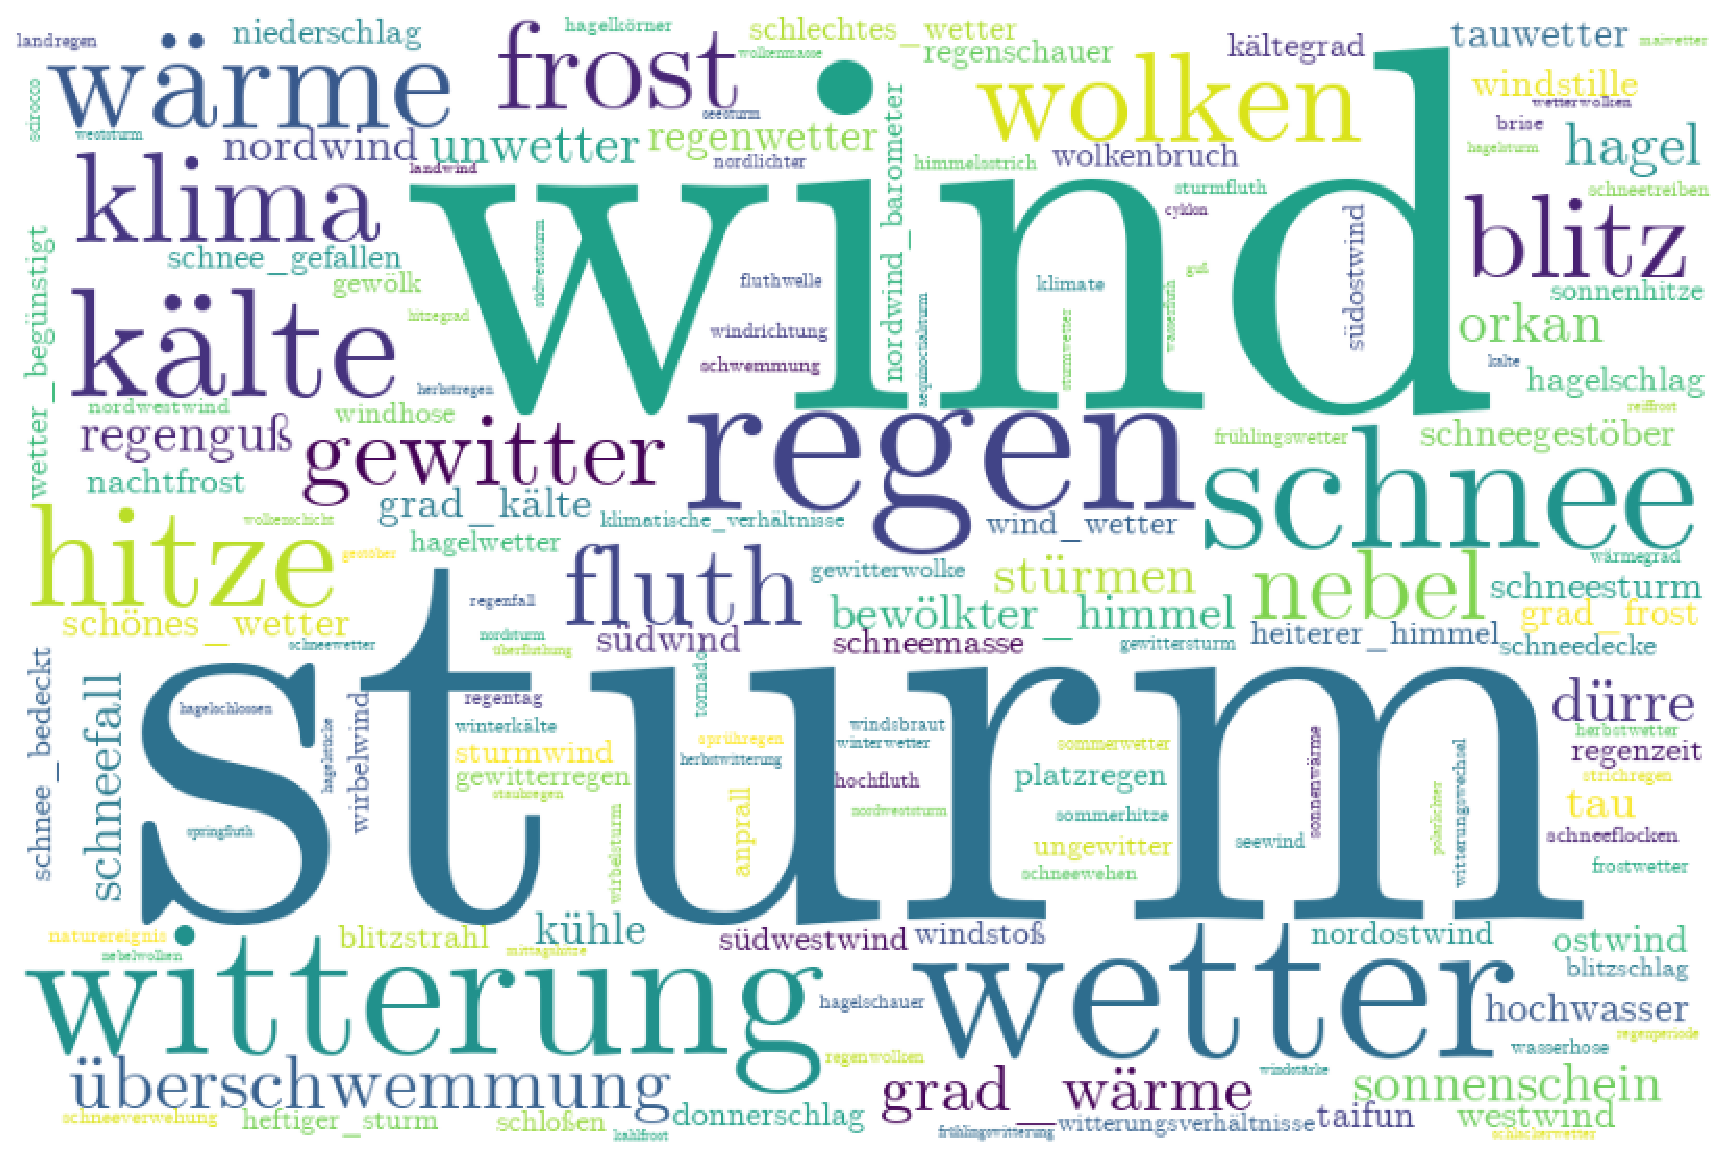
\includegraphics[width=0.9\textwidth]{images/wordcloud_general.pdf}
    \caption{Nuage des mots-clés dans le corpus}
    \label{fig:wordcloud}
\end{figure}

Tout d'abord, on peut poser la question suivante : \og la fréquence dont l'on parle du climat reste-t-elle stable ? \fg{}. Evidemment, le nombre de mots-clés par an augmente au cours du siècle au fur et à mesure que la quantité de l'information devient plus importante (cf. la figure \ref{fig:text_mass}). Pour en tenir compte, le nombre des mots-clés peut être pondéré par la masse totale du texte et présenté sur un graphique. La figure \ref{fig:entities_per_mass} montre la quantité des mots-clés en relation au nombre total de caractères pour chaque année, celui-ci étant une estimation grossière des évolutions de la quantité de l'information. On voit que le nombre d'entités en proportion de la masse textuelle reste relativement stable pendant la période observée. Il existe des pics locaux, plus notamment en 1827, mais en gros, la proportion des entités est toujours dans le même ordre de magnitude. La hausse de l'an 1827 semble être causée par une présence des observations météorologiques dans cette année. Ces observations sont souvent incluses dans d'autres articles à cause d'une erreur (ou un choix) de segmentation et échappent alors au filtre de la qualité d'OCR, car la majeure partie de l'article est toujours lisible. Outre ce biais chronologique, la figure \ref{fig:entities_per_mass} peut être donc interprété comme un indice d'une stabilité relative de la représentation du climat pendant toute la période observée.

\begin{figure}[h]
    \centering
    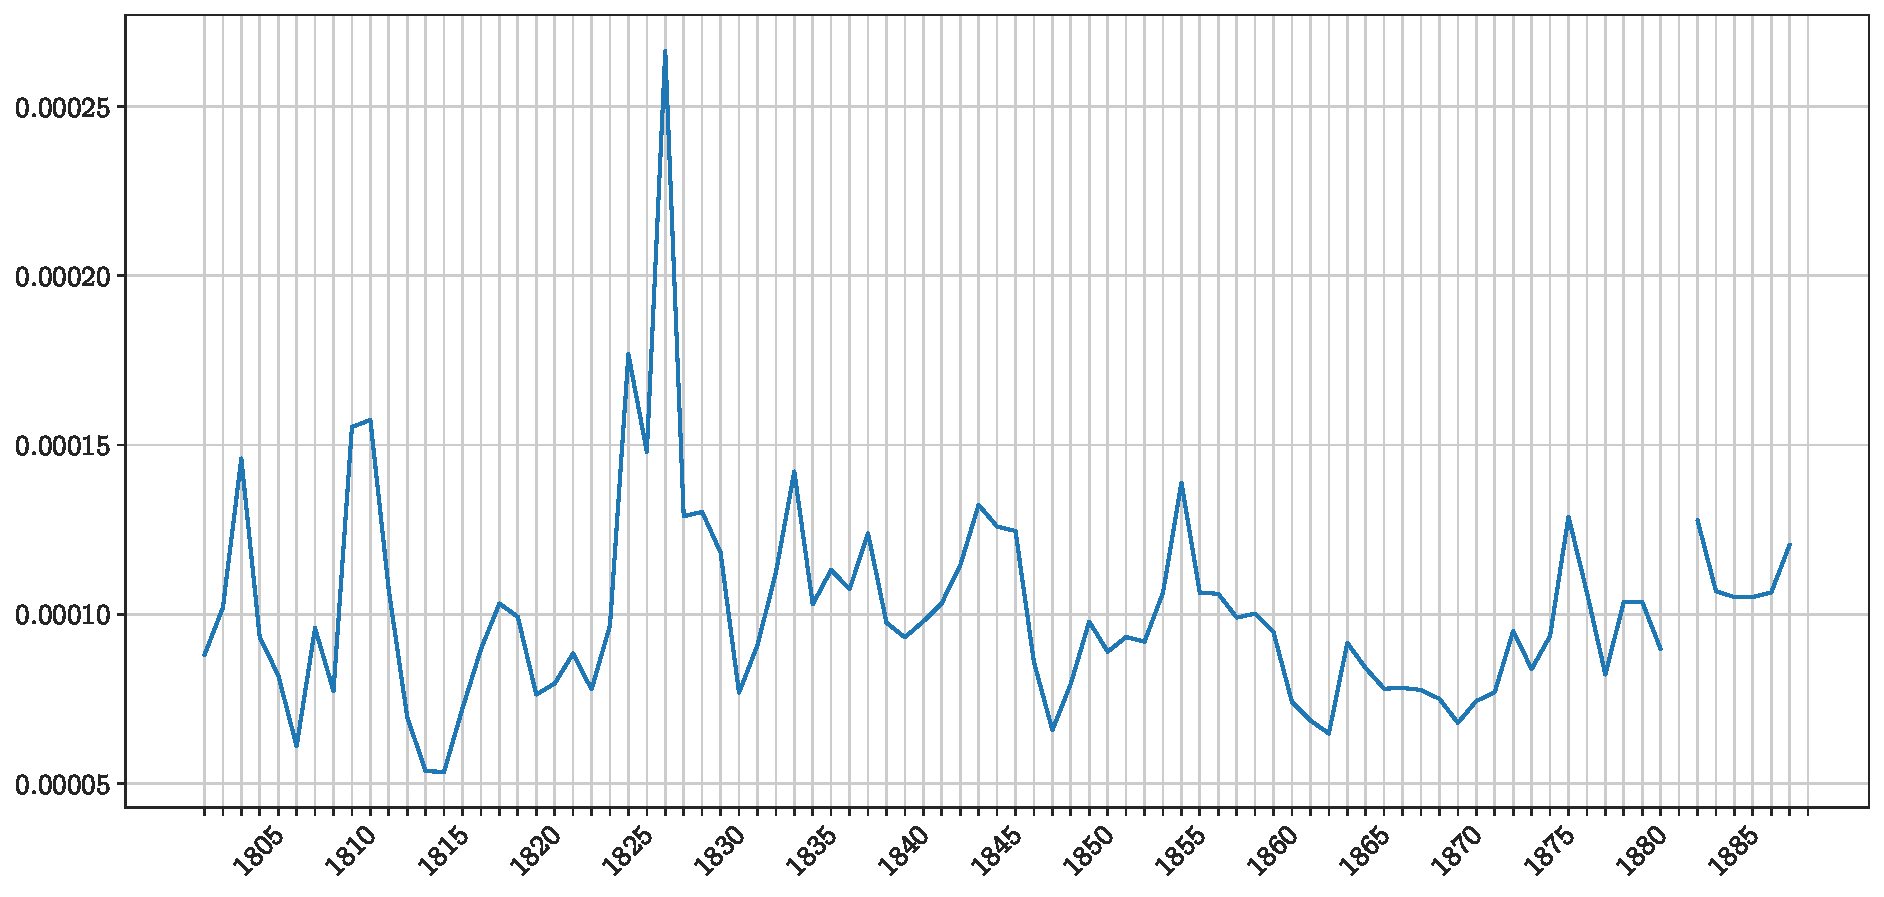
\includegraphics[width=\textwidth]{images/entities_per_mass.pdf}
    \caption{Nombre de mots-clés par rapport à la masse textuelle en caractères}
    \label{fig:entities_per_mass}
\end{figure}


%\subsubsection{}

Il est également possible d'observer la fréquence d'un mot donné et de faire des comparaisons entre différents mots. par exemple, la figure \ref{fig:wetter_witterung_klima} montre la fréquence relative des mots-clés \textit{Klima}, \textit{Wetter}, \textit{Witterung} (climat, le temps, conditions météorologiques) d'une manière relative, i.e. leur proportion de toutes les occurrences d'une année donnée, comme sur les figures \ref{fig:headings_places} et \ref{fig:headings_other}. Là encore, la fréquence d'occurrence semble rester assez stable pour les trois mots et on peut en conclure que les catégories terminologiques les plus larges liées au climat ont une présence constante dans le journal au cours de la période considérée. Selon les changements locaux les plus importants, on remarque le pic du mot \textit{Wetter} dans les années 1860. Un regard plus attentif aux occurrences de \textit{Wetter} dans cette fenêtre temporelle révèle que ils se trouvent en grande majorité (302 fois en 1864-1866) dans les articles intitulés \textit{Börsen- und Handelsnachrichten}, i.e. les actualités boursières et commerciales (cf. le tableau \ref{tab:common_headings}) qui relatent, entre autres informations, des conditions météorologiques dans d'autres villes.\footnote{Le début de cette tendance correspond aux développements communicationnels à Riga au début des années 1860 - il est probable que l'arrivée du transport ferroviaire et du télégraphe ont suscité un plus grand intérêt aux conditions météorologiques en temps réel (cf. aussi la setion \ref{contenu})}. Cependant, il ne s'agit pas d'observations météorologiques dans le sens \og scientifique \fg{}, mais plutôt de courtes remarques: les autres mots-clés ne sont pas mentionnés si souvent que le temps, et une analyse rapide du contexte immédiat du mot en question montre qu'il est le plus souvent décrit avec un seul adjectif, p.ex \textit{schön}, \textit{ruhig}, \textit{trüb} ou \textit{unverändert} (beau, calme, maussade, inchangé).

% ref to the immediate context section?

\begin{figure}[h]
    \centering
    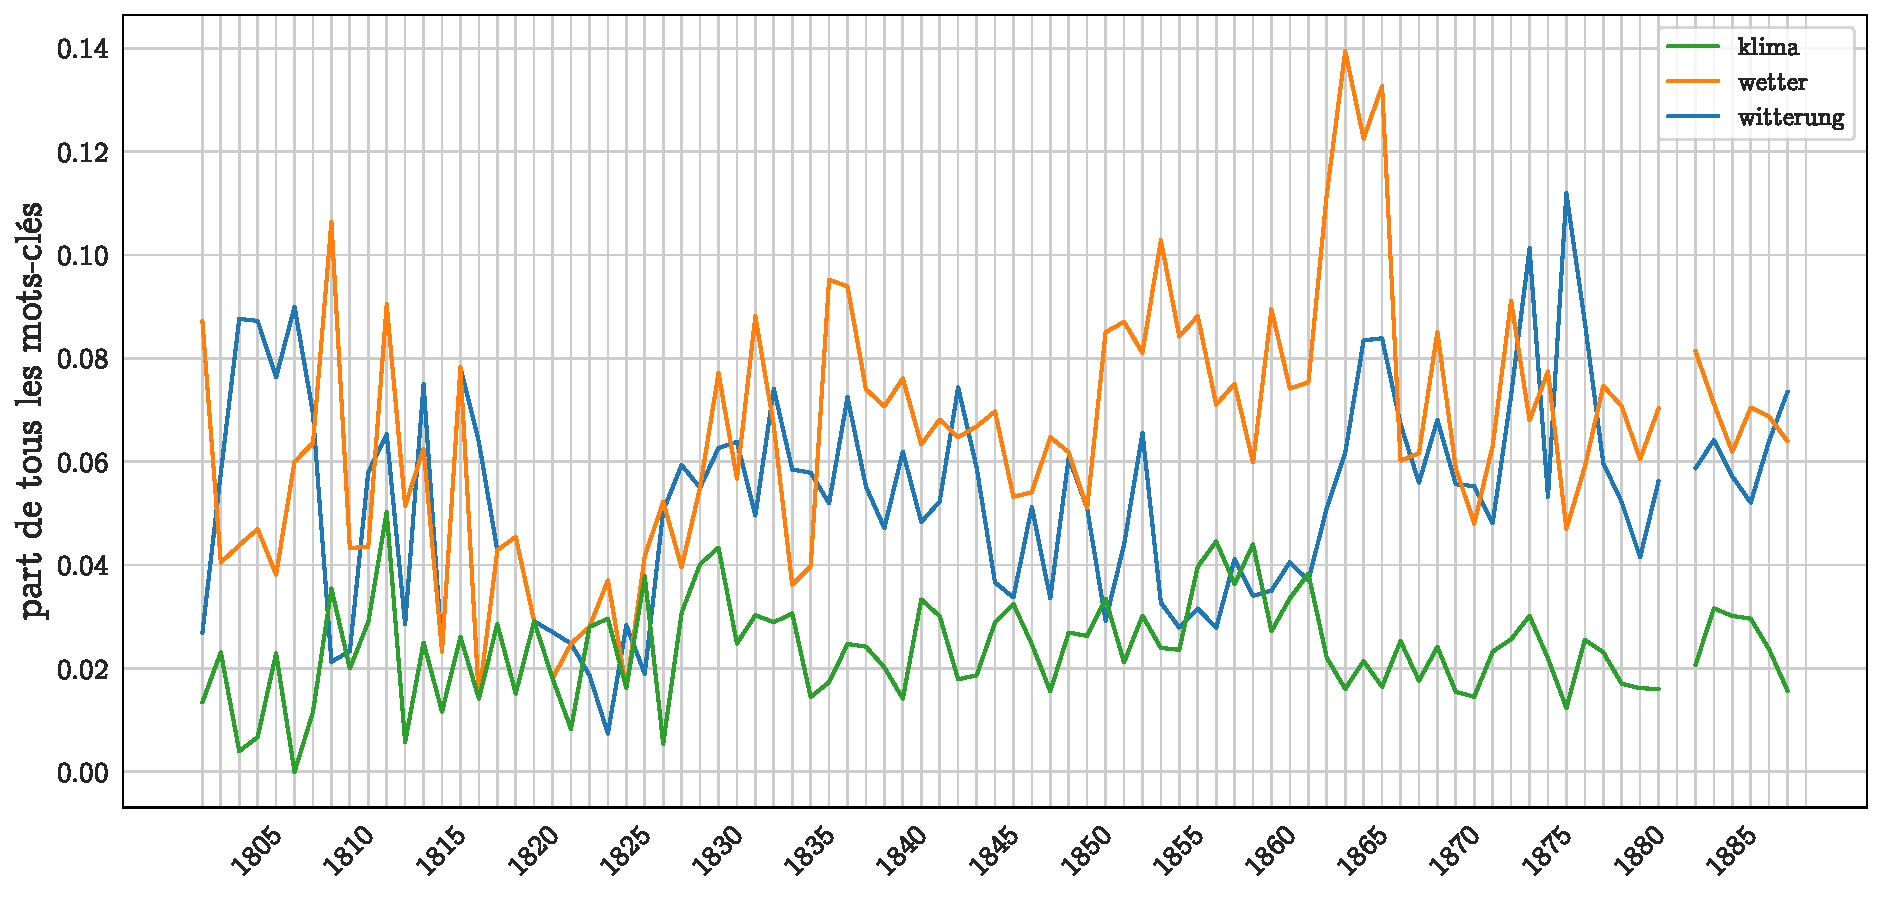
\includegraphics[width=\textwidth]{images/wetter_witterung_klima.pdf}
    \caption{Fréquence relative des mots-clés \textit{climat}, \textit{le temps}, \textit{conditions météorologiques}}
    \label{fig:wetter_witterung_klima}
\end{figure}

Dans le même sens, la distribution des 10 mots-clés les plus populaires est présenté sur la figure \ref{fig:top_keywords10}. En général, l'importance relative de ces mots reste stable pendant la période observée. Le fait que les fluctuations plus importantes se trouvent dans le premier tiers du siècle semble indiquer qu'ils découlent de la faible quantité des données, tandis que la partie du siècle plus riche en données voit une stabilisation de la fréquence de ces mots-clés.

\begin{figure}[h]
    \centering
    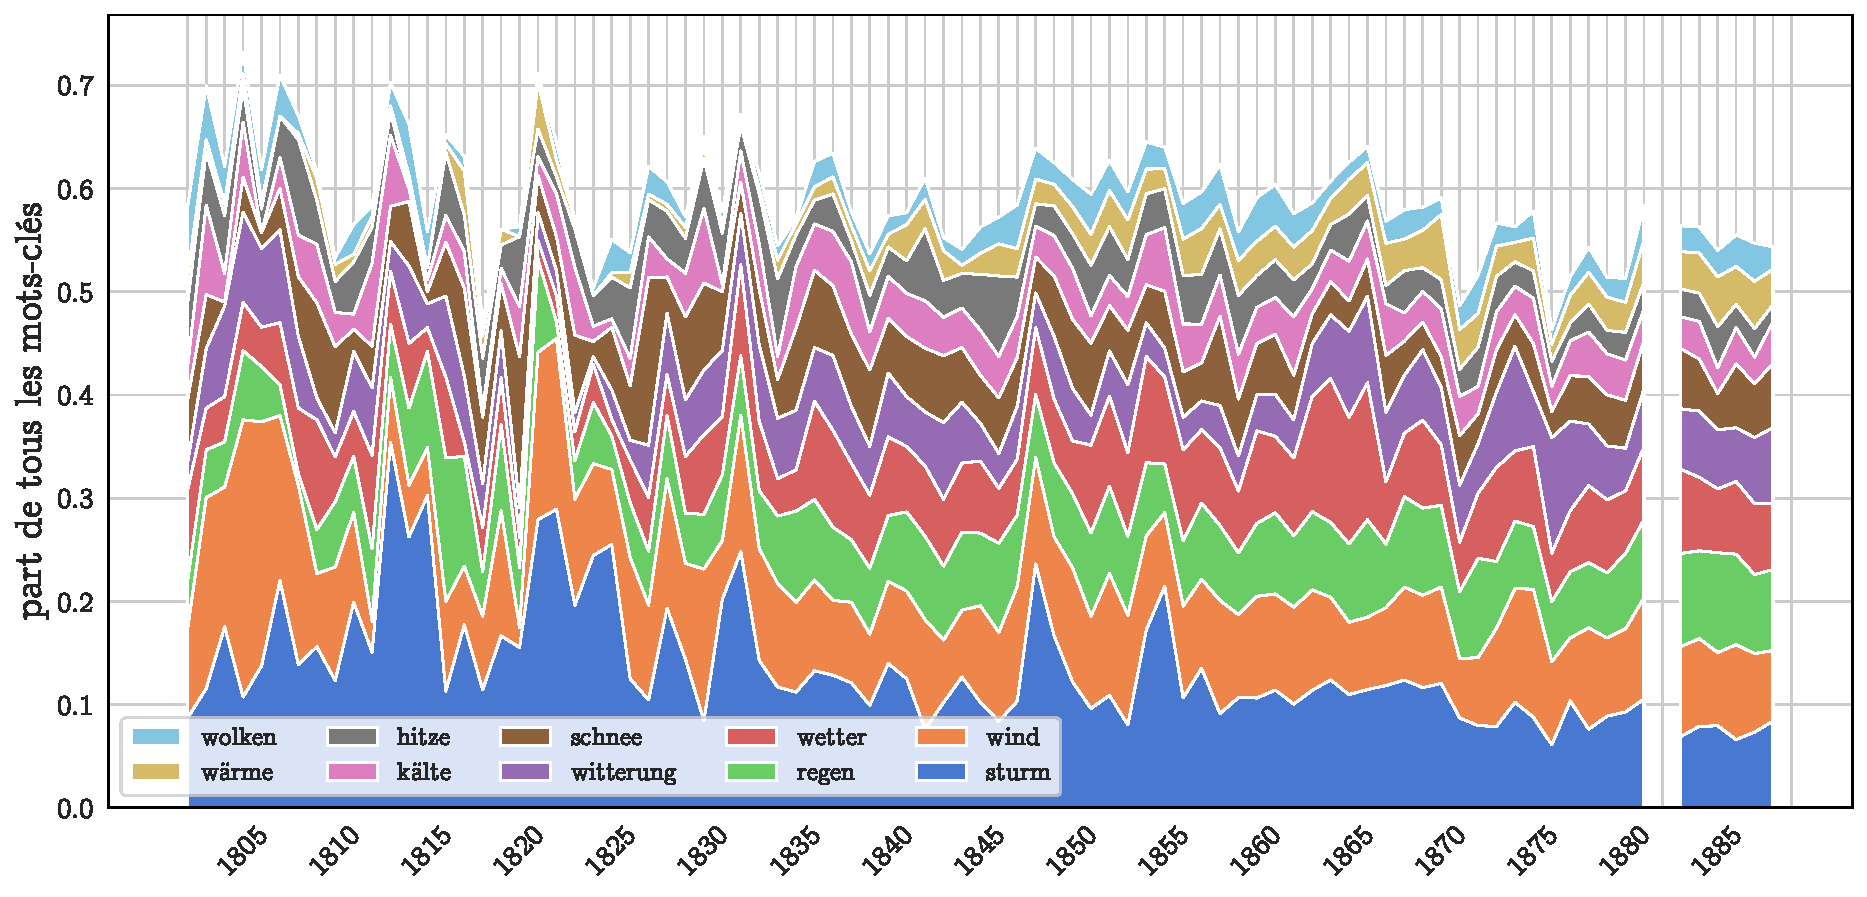
\includegraphics[width=\textwidth]{images/10_most_frequent_ents.pdf}
    \caption{Fréquence relative des 10 mots-clés les plus fréquents}
    \label{fig:top_keywords10}
\end{figure}

Alors que les fréquences des mots-clés les plus fréquents affichent une relative stabilité, les enquêtes sur les mots moins répandus peuvent révéler des poussées temporaires d'intérêt. La figure \ref{fig:orkan_taifun_tornado} démontre les occurrences des mots \textit{Orkan}, \textit{Taifun}, \textit{Tornado} et \textit{Scirocco} sur une échelle absolue. Il se trouve que les occurrences du mot \textit{Orkan} sont reparties de manière assez homogène, mais celles de \textit{Taifun} sont concentrées sur les années 1860 et que \textit{Tornado} ne fait que quelques apparitions, principalement entre 1867 et 1874. En analysant les titres d'articles qui contiennent le mot \textit{Taifun} dans cette fenêtre temporelle, une dominance des actualités de l'Asie est immédiatement perceptible. Il est probable que cette poussée d'intérêt est directement liée aux typhons dévastateurs qui ont ravagé le Japon et la Chine dans les années 1860.\footcite{yim_reconstruction_2007}

Les typhons ne sont pas les seuls phénomènes climatiques tropicaux qui trouvent leur chemin vers les lecteurs du \textit{Rigasche Zeitung}. Le Sirocco (aussi appelé \textit{Scirocco}) est un vent saharien qui peut atteindre la vitesse d'un ouragan et parvenir jusqu'au côte nord de la Mediterranée. Les nouvelles sur le Sirocco viennent donc principalement de l'Italie et ses villes. A trois occasions, un article entier est consacré au Sirocco.\footnote{RZ 19/10/1855 (\texttt{id: 128124}) ; RZ 27/19/1855 (\texttt{id: 128224}) ; RZ 08/04/1869 (\texttt{id: 190735})}

\begin{figure}[h]
    \centering
    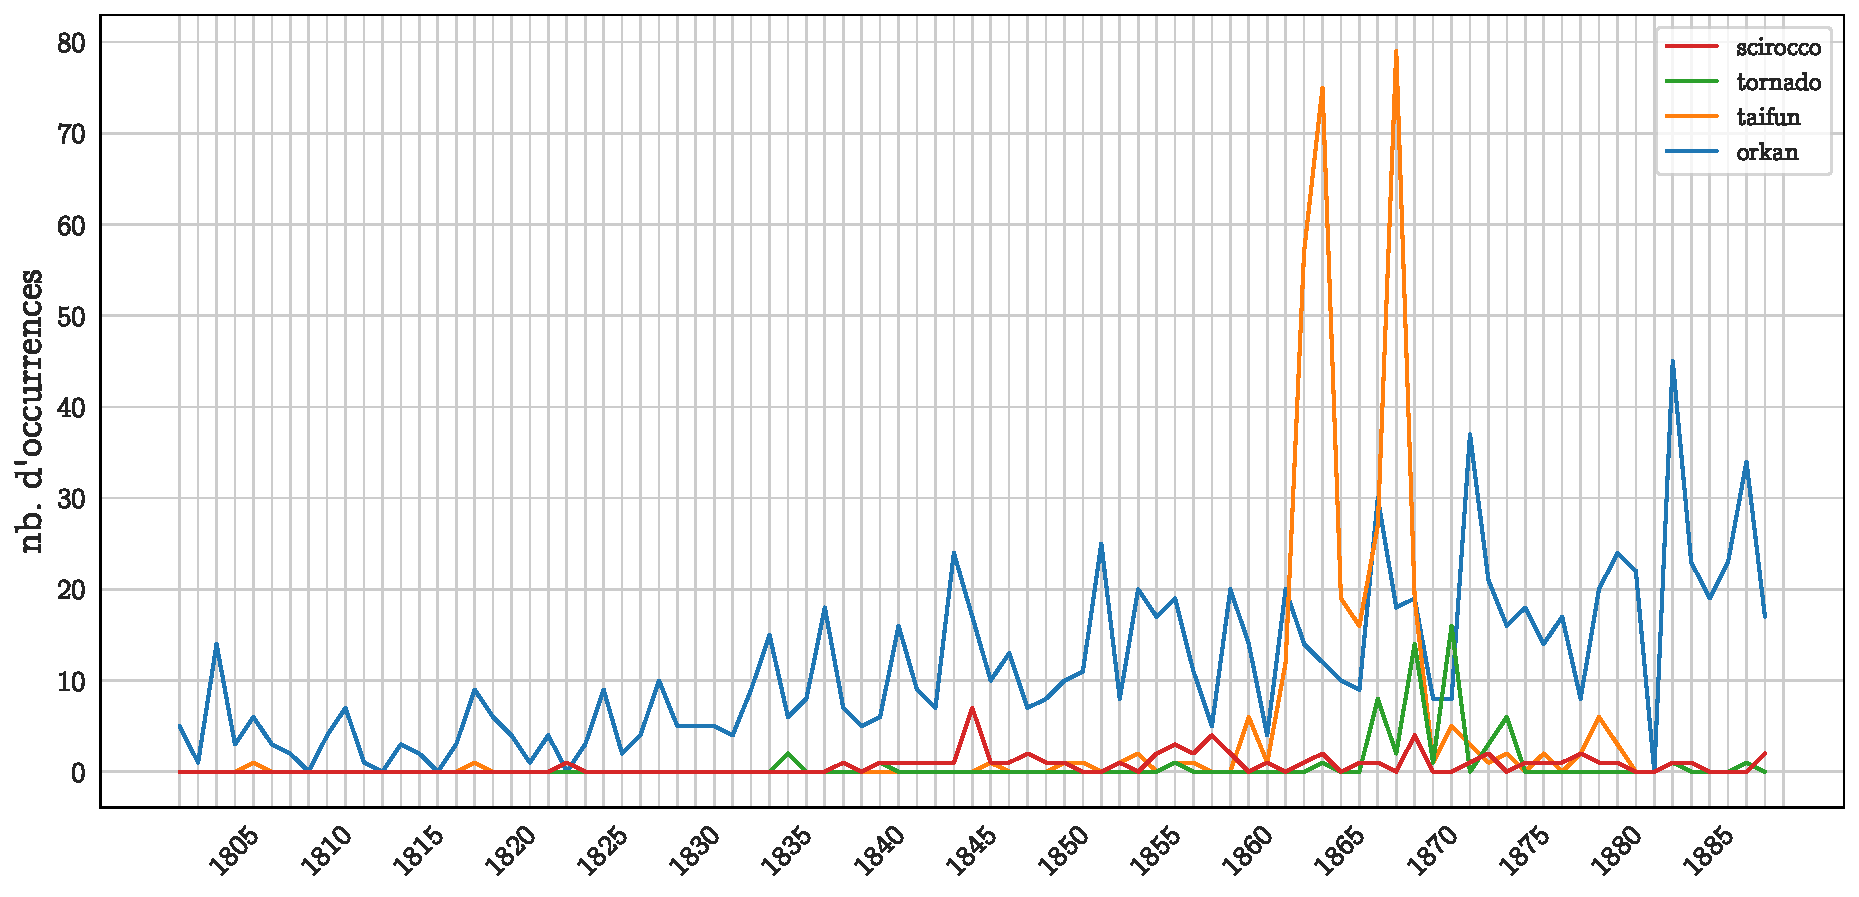
\includegraphics[width=\textwidth]{images/orkan_taifun_tornado.pdf}
    \caption{Fréquence absolue des mots \textit{ouragan}, \textit{typhon}, \textit{tornade}}
    \label{fig:orkan_taifun_tornado}
\end{figure}

D'autres phénomènes présentent encore une image différente. Par exemple, la grêle est le plus souvent mentionnée dans le contexte de l'empire russe ou de la région baltique. Un tiers de tous les articles qui évoquent la grêle ou l'un de ses synonymes, sont intitulés \textit{Inland}. Il parait que pendant certaines périodes, des nouvelles des grêles dévastatrices ont circulé dans la presse - par exemple la figure \ref{fig:hagelschlag} montre que dans le contexte immédiat du mot-clé \textit{Hagelschlag} (coup de grêle), se trouvent les mots \textit{Gouvernement} et \textit{Kreise} (des divisions administratives), ainsi que \textit{shaden}, \textit{schaden\_angerichtet}, \textit{vernichtet}, \textit{Fenstercheiben} et \textit{Getreide} (dommages, dommages causés, détruit, vitres, céréales). \label{about:hagel}

\begin{figure}[h]
    \centering
    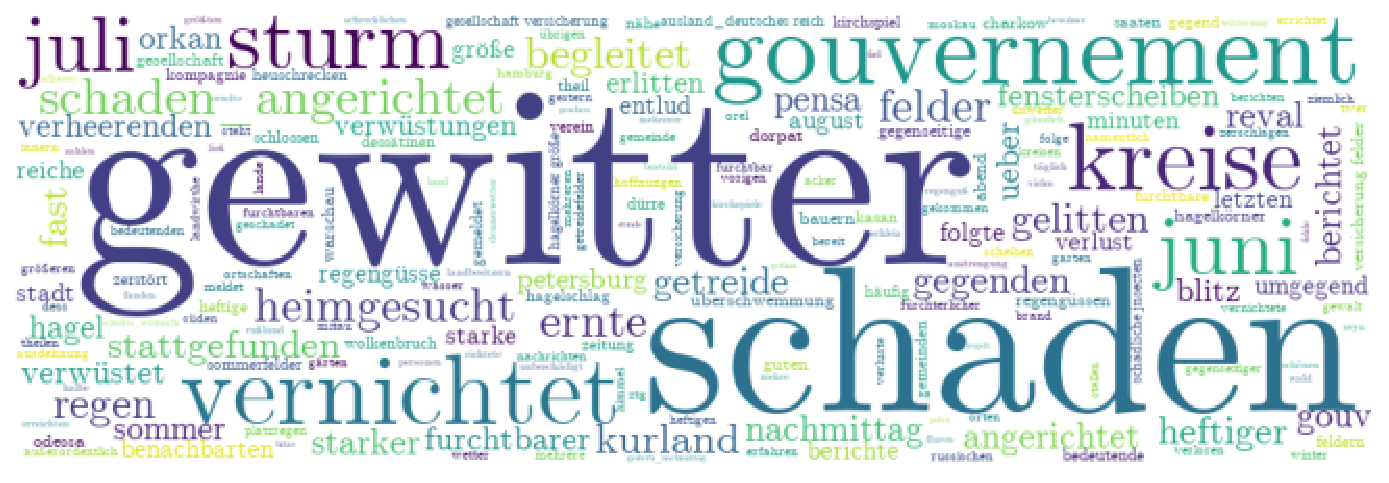
\includegraphics[width=0.9\textwidth]{images/wordcloud_hagelschlag.pdf}
    \caption{Contexte immédiat du mot-clé \textit{Hagelschlag} (coup de grêle)}
    \label{fig:hagelschlag}
\end{figure}

En regardant la fréquence absolue de la grêle et ses synonymes (figure \ref{fig:hagel}), on remarque immédiatement un pic soudain dans l'année 1872. Il s'avère que la poussée est causée en grande partie par deux articles qui contiennent au total 20 mentions de grêle, ainsi qu'un grand nombre d'autres mots-clés. Ces articles, à une semaine d'intervalle, racontent dans le détail une tempête de grêle qui a ravagé Riga et ses alentours le 10 mai 1872.\footcite[Pour plus de détails sur cette tempête particulière, cf :][]{plath_kuidas_2021} Le deuxième article semble en fait être un supplément du journal, entièrement consacré à ces événements. La grêle fût accompagné par un tourbillon de poussière et infligea des dommages considérables.\footnote{\og Un événement naturel si rare a frappé une partie de notre province, notamment notre ville et ses environs, et a laissé des traces de destruction si cruelles qu'il semble justifié de mettre par écrit les impressions encore vives et de laisser une image de ses conséquences, même pour les temps ultérieurs, \fg{} rapporte le correspondant du \textit{Rigasche Zeitung} émotionnellement. RZ 19/03/1872 (\texttt{id: 208050})} Parmi les dommages constatés, arbres déracinés, fenêtres cassées, jardins en ruine ont été signalés, ainsi que la mort de plusieurs personnes.\footnote{\og Je viens d'apprendre avec certitude que quatre domestiques du château de Wenden ont été entièrement détruits, et qu'il ne reste pas une poutre sur l'autre. Une femme a été tuée et on n'a retrouvé jusqu'à présent qu'un bras ou une jambe d'une gardienne, dont on cherche le corps. On dit aussi que les domestiques de Freydenhof et de Lindenhof ont été détruits et qu'un petit bois de bouleaux a été totalement déraciné et bouleversé. \fg{} RZ 13/03/1872 (\texttt{id: 207965})} Les deux articles sont un curieux mélange de narrations émotionnelles probablement un peu exagérées et de descriptions minutieuses de la nature du phénomène, communicant au lecteur les changements de la température et de la pression atmosphérique et décrivant la taille précise des plus gros grêlons trouvés.

\begin{figure}[h]
    \centering
    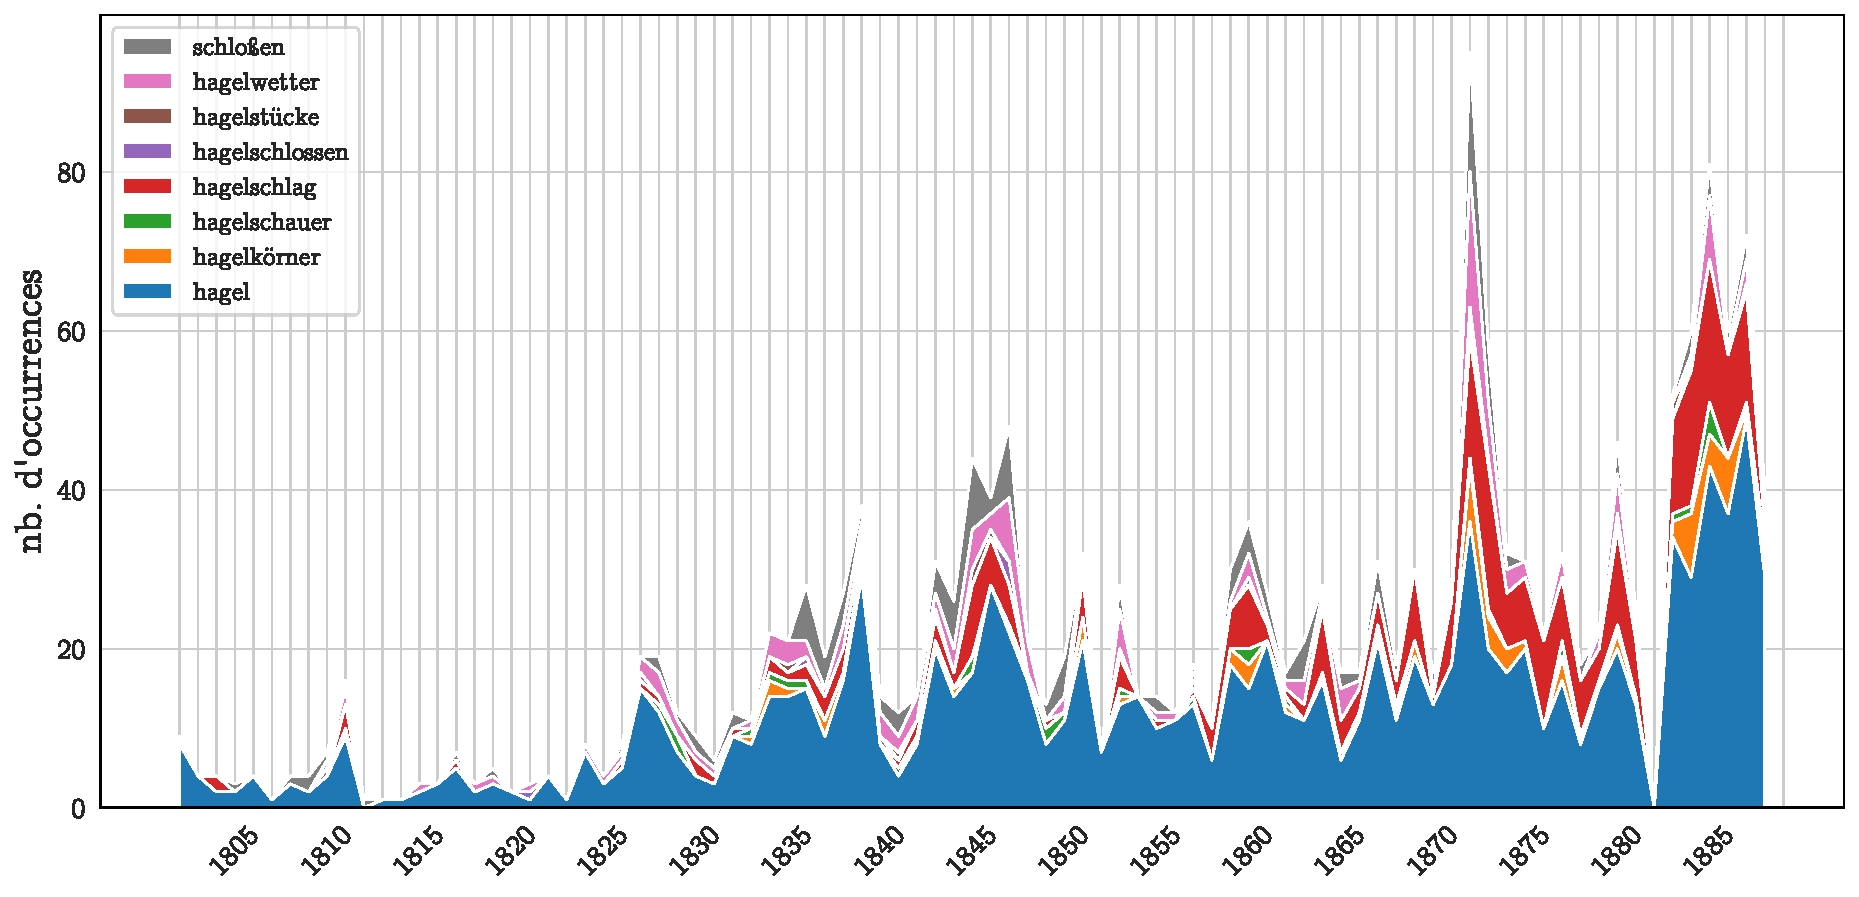
\includegraphics[width=\textwidth]{images/hagel.pdf}
    \caption{Fréquence absolue de \textit{grêle} et ses synonymes}
    \label{fig:hagel}
\end{figure}

Comme le montre cet exemple, les tendances temporelles des mots clés peuvent également servir à la détection des événements uniques qui peuvent ensuite être analysés à l'aide des métadonnées. Toutefois, il faut prêter attention aux réserves que peut susciter un petit nombre de textes contenant un nombre élevé de mots-clés. En regardant la figure \ref{fig:hagel}, l'on pourrait d'abord avoir l'idée que l'année 1872 a connu d'abondantes tempêtes de grêle, mais en réalité, cette dynamique est surtout due à une forte surreprésentation du phénomène dans deux articles.

Le dernier exemple de ce chapitre démontre les pièges qui peuvent surgir si l'analyse quantitative est trop superficielle. La fréquence du mot \textit{Sturm} (tempête) et ses synonymes est la plus élevée en 1855 avec 457 occurrences, tandis que la fréquence moyenne en 1802-1888 est de 161 par an. Une simple analyse montre tout de suite la raison de ce pic. En comparant les mots voisins de \textit{Sturm}, on voit les différences entre le nuage de mots calculé sur toute la période et le nuage de mots basé uniquement sur les données de 1855 (figure \ref{fig:sturm_wordclouds}. Les mots les plus présents dans le nuage général semblent indiquer que de l'information sur les tempêtes a été souvent communiquée juste après un événement important dans une autre ville (\textit{Stadt}, \textit{letzten}, \textit{Nacht} - ville, dernière, nuit). D'autres mots évoquent un lien avec la navigation (\textit{Schiff}, \textit{Küste}, \textit{Hafen}, \textit{Wasser} - navire, côte, port, eau) et les caractéristiques de fortes tempêtes (\textit{heftigen}, \textit{wüthete}, \textit{furchtbarer} - violent, faire rage, terrible). Entre 1802 et 1888, les mots de contexte donnent une image assez cohérente de la représentation des tempêtes en tant qu'événements météorologiques dans le corpus.

\begin{figure}[h!]
\centering
\begin{subfigure}
    \centering
    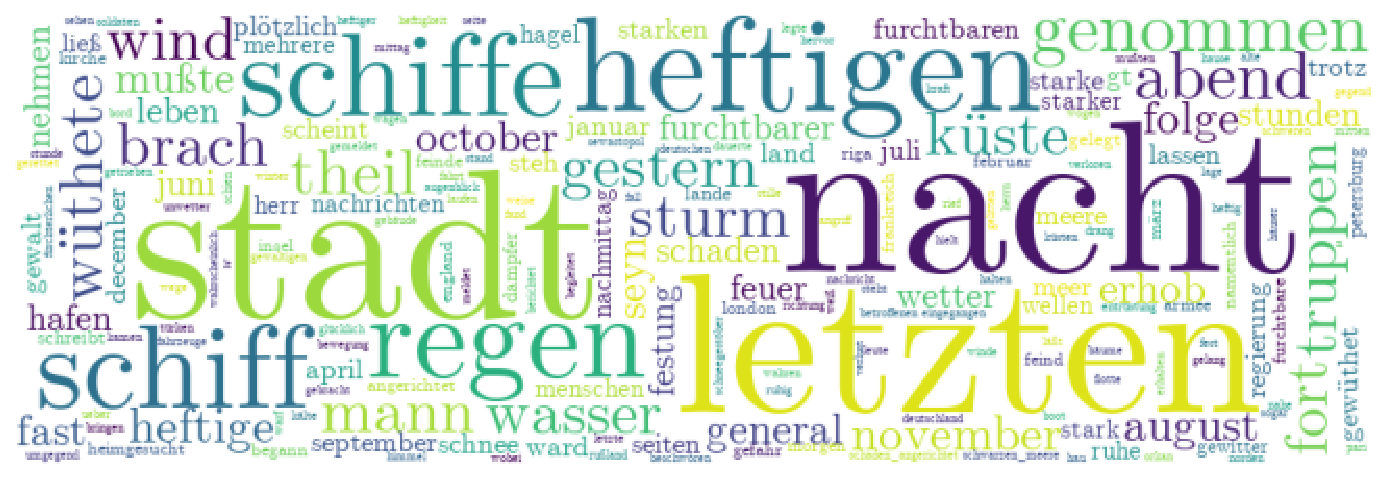
\includegraphics[width=0.9\textwidth]{images/wordcloud_sturm.pdf}
\end{subfigure}
\begin{subfigure}
    \centering
    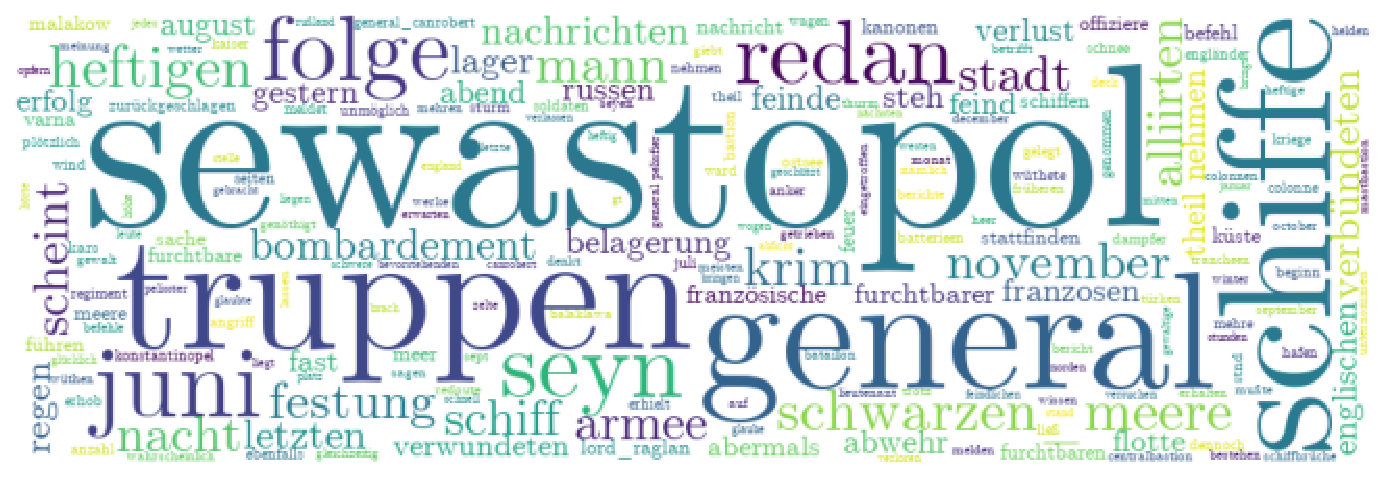
\includegraphics[width=0.9\textwidth]{images/wordcloud_sturm_1855.pdf}
\end{subfigure}
\caption{Le contexte immédiat de \textit{tempête} pour toute la période et en 1855}
\label{fig:sturm_wordclouds}
\end{figure}

Par contre, le second nuage trahit d'emblée en quoi il serait faux de considérer le pic de 1855 comme un indice de tempêtes violentes ou plus fréquentes. Les mots \textit{Sewastopol}, \textit{Truppen}, \textit{General}, \textit{Bombardement}, \textit{Belagerung}, \textit{Krim}, \textit{Franzosen} etc. font clairement apparaître qu'il s'agit du sens militaire du mot \textit{Sturm} (cf. la page \pageref{synonymes}, dont la fréquence a été augmentée par la guerre de Crimée.

La notion du contexte est donc très importante pour la lecture distante du climat et sera traitée dans la partie suivante. En parallèle, le chapitre actuel démontre les diverses possibilités d'analyse quantitative au niveau des mots-clés. Les distributions temporelles des mots-clés révèlent de l'information sur la quantité et la nature de la représentation des événements climatiques. Dans certains cas, il est possible de identifier des événements uniques, ce qui permet d'accéder à une analyse qualitative des sources.

\clearpage


\section{Sujets du climat} \label{topic_modeling}

Comme l'a montré le chapitre précédent, les textes contenant des mots-clés pertinents peuvent être de nature très différente, certains n'étant même pas liés au climat. Etant donné que les descriptions associées au temps et au climat sont évidemment très différentes, le but de ce chapitre est de modéliser les catégories principales des textes contenant des mots-clés \og climatiques \fg{}.

La modélisation de sujets est un ensemble de techniques qui permettent détecter automatiquement les \og sujets \fg{} qui apparaissent dans une collection de documents. Il s'agit de méthodes non-supervisées, ce qui veut dire qu'elles fonctionnent sans données étiquetées. Il n'est pas nécessaire de prédéterminer les sujets associés aux textes que l'on s'attend à trouver - les sujets sont modelés selon la distribution des mots dans les textes. Ainsi, une co-occurrence récurrente d'un nombre de mots a la probabilité d'être définie comme un sujet. Les noms des sujets trouvés par l'algorithme dépendent donc de l'interprétation humaine. Le caractère non supervisé de ces méthodes représentent donc leur principal avantage, parce qu'ils permettent d'explorer la nature des textes sans connaissance préalable du contenu. Pour un grand corpus, des attentes erronées concernant les thèmes évoquées pourraient même gravement fausser les résultats.

Il existe plusieurs méthodes de modélisation des sujets, qui se distinguent les unes des autres principalement par la nécessité de disposer d'un nombre prédéterminé de sujets. Une première tentative a été réalisée avec l'algorithme LDA\footcite{jelodar_latent_2019}, qui s'est toutefois avéré insatisfaisant. Les sujets obtenus n'étaient pas interprétables et avaient tendance à se chevaucher fortement, avec un nombre quelconque de sujets prédéterminés. Après quelques expériences, j'ai découvert que les meilleurs résultats sont obtenus par une méthode relativement nouvelle appelée \textit{top2vec}.\footcite{angelov_top2vec_2020} \textit{Top2vec} est basé sur \textit{word2vec} qui a été utilisé dans le chapitre précédent pour vectoriser les mots du corpus. Tout d'abord, \textit{top2vec} calcule des \textit{embeddings} supplémentaires pour les documents - ceux-ci sont basés sur les valeurs des \textit{embeddings} de mots dans le document. Les vecteurs hyperdimensionnels de documents obtenus sont ensuite projetés dans un espace bidimensionnel avec l'algorithme UMAP (de la même manière que pour la figure \ref{fig:keyword_umap}). Enfin, les vecteurs bidimensionnels obtenus sont regroupés par HDBSCAN, un algorithme de regroupement (\textit{clustering}) qui trouve les zones où les vecteurs sont le plus densément regroupés.\footcites{campello_density-based_2013} Cela repose sur l'hypothèse que les documents ayant des vecteurs similaires (c'est-à-dire proches les uns des autres dans l'espace) sont similaires dans leur contenu sémantique. Chaque regroupement trouvé par HDBSCAN est donc considéré comme un \og sujet \fg{}. Les documents ne doivent pas nécessairement appartenir à un seul sujet. Par exemple, les vecteurs qui se trouvent entre deux zones denses sur la projection UMAP sont considérés comme appartenant partiellement aux deux \textit{clusters}, celui dont il est le plus proche étant le sujet principal. Les sujets résultants sont définis par les mots qui leur sont les plus caractéristiques.

Afin d'utiliser \textit{top2vec} sur des descriptions climatiques et météorologiques, il est d'abord nécessaire d'extraire les parties des articles qui contiennent les mots-clés pertinents. Ces parties de texte deviennent alors l'entrée de l'algorithme de modélisation des sujets. Les segments ont été créés en tenant compte de certains paramètres : dans les textes tokenisés, les 20 mots qui précèdent et suivent un mot-clé ont été inclus dans l'intervalle. En outre, si la distance entre deux mots-clés était égale ou inférieure à 100 tokens, tous ces tokens étaient inclus dans l'intervalle. Cela devrait permettre de créer des segments plus cohérents et plus longs dans les cas où les mots-clés mentionnés ne sont pas étroitement groupés. Enfin, seuls les segments qui incluent trois mots-clés ou plus sont utilisés pour la modélisation du sujet. Cela réduit la variance textuelle en omettant les mots-clés isolés - plusieurs mots-clés apparaissant ensemble augmentent considérablement la probabilité que le mot-clé ne soit pas utilisé dans une métaphore, par exemple.\footnote{\texttt{./climdist/train\_top2vec.py}, fonction \texttt{build\_spans}, paramètres \texttt{window}, \texttt{stretch}, \texttt{min\_len}} En utilisant ces paramètres, \textbf{12 291 segments} ont été détectés dans l'ensemble du corpus.

Les paramètres décrits ont un effet important sur l'éventuelle modélisation du sujet car ils tentent d'isoler efficacement les descriptions climatiques et météorologiques du texte environnant. Cela n'est malheureusement pas toujours possible avec un ensemble de règles fixes, car les descriptions réelles dans le corpus varient considérablement en longueur et sont souvent entourées de toutes sortes de textes différents. Comme décrit dans le chapitre \ref{sources}, la séparation des articles est très dépendante des décisions humaines et de nombreux articles contiennent une variété de nouvelles et de messages. Ainsi, il est inévitable que certains des segments résultants comprennent des parties non pertinentes de l'article et que certaines descriptions pertinentes plus longues soient divisées en plusieurs segments. Des expérimentations supplémentaires avec ces valeurs pourraient donc potentiellement aider à améliorer les résultats à l'avenir.

Les segments sont utilisés pour entraîner le modèle \textit{top2vec}.\footnote{Le script d'entraînement se trouve dans \texttt{./climdist/train\_top2vec.py} ; le modèle final est dans \texttt{./data/models/top2vec/}} Celui-ci attribue un vecteur de document à 300 dimensions à chaque segment et ne prend en compte que les mots qui apparaissent au moins 20 fois. Le nombre original de sujets détectés par l'algorithme est de 46 \label{46_topics}, mais \textit{top2vec} permet de réduire ce nombre pour obtenir une vue plus générale. Cela se fait en fusionnant les \textit{clusters} les plus similaires jusqu'à ce que le nombre de sujets souhaité soit atteint. Après avoir expérimenté avec différents nombres, j'ai trouvé que le nombre optimal de sujets qui est facilement interprétable tout en gardant un niveau de détail suffisant, est de 16.\footnote{Ces expérimentations, ainsi que les visualisations suivantes se trouvent dans le \textit{notebook} \newline \texttt{./notebooks/topics.ipynb}} Après un examen des mots les plus caractéristiques de chaque sujet, la distribution temporelle de celui-ci, ses mots-clés les plus répandus et les titres des articles dans lesquels les segments sont contenus, ainsi que plusieurs exemples de textes, j'ai attribué un nom à chacun d'entre eux.

Sur les 16 sujets, quatre peuvent être considérés comme des faux-positifs. Cela signifie qu'ils contiennent les mots-clés pertinents mais que le sujet en général indique qu'ils sont utilisés soit dans un sens métaphorique, soit qu'ils résultent de segments \og bruyants \fg{}. Par exemple, deux sujets contiennent principalement des textes de nature littéraire et souvent inclus dans des romans qui étaient parfois publiés en partie dans le \textit{Rigasche Zeitung}. Deux autres sujets sont de nature politique, souvent inclus en raison du sens métaphorique du mot \textit{Sturm} - plus particulièrement dans son sens militaire (voir la page \pageref{fig:sturm_wordclouds}). Il en reste donc \textbf{12 sujets} différents que j'ai étiquetés. Ce qui suit est une brève description de chacun des 12 sujets, tandis que les détails - fréquence temporelle, mots-clés caractéristiques (tant météorologiques que généraux), les titres d'articles les plus répandus et exemples textuels - se trouvent dans \nameref{annexe}. Les exemples dans l'annexe sont choisis parmi les 1-5 segments dont les vecteurs sont les plus centrales dans le groupe (sujet) auquel ils appartiennent.

\vspace{1ex}
\begin{enumerate}
    \item \textbf{\nameref{topic1_chimie-vegetation}} - Ce thème, celui qui apparaît le plus fréquemment, est moins cohérent que les suivants et il contient en fait plusieurs types de textes. Il y a des descriptions chimiques qui sont incluses en raison de la nature générale de mots comme \textit{nature} et \textit{chaleur}, et qui pourraient donc être considérées comme des faux positifs. Un autre type de segments traite de l'agriculture de manière technico-scientifique. Enfin, les textes sur la récolte sont aussi parfois classés comme appartenant à ce thème, alors qu'ils pourraient en fait appartenir au sujet suivant.
    
    \item \textbf{\nameref{topic2_recolte}} - Ce thème consiste principalement en des nouvelles sur les récoltes qui constituent une partie importante de l'information économique du journal. Parmi les mots les plus caractéristiques des segments correspondants, on trouve par exemple : \textit{récolte}, \textit{sécheresse}, \textit{céréales d'été}, \textit{champs}, \textit{médiocre}, \textit{croissance}, \textit{seigle}, \textit{pommes de terre}, etc.  Le mot-clé climatique le plus courant dans ces segments est \textit{pluie} (sans surprise), suivi de \textit{conditions météorologiques}, \textit{sécheresse}, \textit{temps}, \textit{neige} et \textit{gel}. La majorité de ces informations ont été publiées dans des articles sur les affaires intérieures, suivis par \textit{Riga}.

    \item \textbf{\nameref{topic3_festivités}} - Ce sujet reflète l'importance de la météo pour les événements publics. En effet, de nombreux rassemblements, festivités, défilés, foires, etc. se déroulant en plein air, leur succès dépendait fortement des conditions météorologiques. Les mots les plus caractéristiques de ce thème sont donc \textit{public}, \textit{musique} \textit{invités}, \textit{théâtre}, \textit{visite}, \textit{feu d'artifice}, \textit{programme} et \textit{malgré}, ce dernier indiquant les événements qui se sont déroulés par mauvais temps. Ces types de descriptions provenaient principalement du niveau local (\textit{Locales}, \textit{Riga}, \textit{Inland}), mais parfois des événements plus importants de l'étranger (\textit{Paris}, \textit{Londres}, \textit{Berlin}) étaient également rapportés.
    
    \item \textbf{\nameref{topic4_commerce}} - Ce sujet est fréquent en nombre, mais apparaît dans un ensemble de textes très spécifiques. La quasi-totalité des occurrences sont contenues dans trois types d'articles (\textit{commerce et transport}, \textit{nouvelles boursières et commercials} et \textit{Riga}) et se concentrent sur deux périodes assez courtes qui correspondent à la publication des deux premières de ces rubriques dans le \textit{Rigasche Zeitung}. Le contexte de ces rapports de routine est caractérisé par des mots comme \textit{chiffres d'affaires}, \textit{envie d'achat}, \textit{livraison}, \textit{affaires}, \textit{avoine}, \textit{prix}, \textit{marchandises}, etc. Comme on le voit dans l'exemple, les informations sur les prix du commerce dans le port étaient souvent liées à une brève notice sur les conditions météorologiques (on remarque que les deux mots-clés les plus fréquents sont juste météo et conditions météorologiques).

    \item \textbf{\nameref{topic6_navigation}} - Ce thème est constitué de rapports sur la navigation, ou plutôt sur ses périls. Des mots comme \textit{navire}, \textit{équipage}, \textit{ancre}, \textit{capitaine}, \textit{bateau à vapeur}, \textit{port}, etc. sont révélateurs de reportages narratifs, dont une part importante concerne des naufrages ou des accidents de mer (\textit{tempête} étant le mot-clé le plus courant). La popularité de \textit{Londres} dans les titres est due à sa centralité dans l'économie maritime du XIX\textsuperscript{e} siècle - de nombreuses nouvelles du monde entier étaient reflétées dans les journaux londoniens. La nature souvent détaillée de ces rapports laisse penser que les lecteurs ont pu apprécier les sensations fortes de ces récits.
    
    \item \textbf{\nameref{topic8_hiver-ferroviaire}} - Ce thème comprend des nouvelles sur les conditions hivernales sévères, mais il est surtout dominé par un seul type d'information : les perturbations des communications causées par la neige (comme le montrent les mots \textit{trafic}, \textit{train}, \textit{retard}, \textit{masse de neige}, \textit{travailleurs}, \textit{poste}, \textit{routes}). Ceci est également illustré par la distribution temporelle du sujet, qui connaît une forte augmentation dans les années 1880. L'exemple ci-dessous illustre comment les nouveaux moyens de transport et de communication, plus avancés, étaient aussi plus sensibles aux caprices du climat.
    
    \item \textbf{\nameref{topic9_inondation}} - Ce sujet-ci relaie l'actualité des inondations et des dégâts qui en résultent, tant en Europe qu'au niveau local. (titres \textit{Allemagne}, \textit{affaires domestiques}, \textit{Riga}, \textit{Paris}, \textit{Londres}, etc). Les mots caractéristiques indiquent les dommages causés aux maisons, aux fermes et aux infrastructures (\textit{effondrés}, \textit{emportés}, \textit{maisons}, \textit{ponts}, \textit{habitants}, \textit{vies humaines}, \textit{détruits}, \textit{réduits en poussière}, etc.). Il est intéressant de noter que ce sujet est réparti plus uniformément dans le temps, avec le plus grand nombre de segments dans les années 1840. Il s'avère également que un nombre de segments regroupés sous ce sujet-ci se traitent en fait des avalanches - probablement à cause des descriptions similaires par rapport aux dommages. Cependant, la partie sur les avalanches ne comporte que 19\% des segments de ce sujet.
    
    \item \textbf{\nameref{topic10_télégrammes}} - Ce sujet est entièrement constitué de télégrammes météorologiques, un type de texte répétitif concentré dans une petite fenêtre temporelle. Pendant quelques années notamment, les télégrammes de l'observatoire météorologique de Saint-Pétersbourg ont été imprimés dans le \textit{Rigasche Zeitung}. Pour des raisons d'espace, je n'ai pas inclus dans l'exemple ci-dessous une liste d'environ 10 villes de l'empire russe et les pressions atmosphériques et températures correspondantes, qui est en fait l'élément principal de ce sujet, faisant de ces noms de lieux certains des mots les plus caractéristiques du sujet (\textit{Kiev}, \textit{Moscou}, \textit{Kasan}, \textit{Mer Noire}, etc.)

    \item \textbf{\nameref{topic12_tempête-grêle}} - Ce thème est clairement dominé par les nouvelles concernant les dommages causés par les tempêtes, dont les tempêtes de grêle sont les plus importantes. Les descriptions des dommages causés aux bâtiments, aux champs, aux jardins, etc. sont un élément important (\textit{toitures}, \textit{déracinées}, \textit{abattues}, \textit{intempéries}, \textit{vitres}, etc.). Les mots-clés climatiques les plus courants sont \textit{tempête}, \textit{grêle}, \textit{tonnerre}, \textit{pluie}, etc., et la plupart des segments se trouvent sous les titres \textit{Affaires doméstiques} et \textit{Riga}. Voir aussi la page \pageref{about:hagel}.
    
    \item \textbf{\nameref{topic13_science}} - Caractérisé par des termes plus généraux et scientifiques (\textit{observations}, \textit{phénomènes}, \textit{causes}, \textit{atmosphère}, \textit{courants}, \textit{théorie}, \textit{professeur}, \textit{météorologie}), ce thème contient des textes qui analysent le climat et la nature de manière empirique. Notamment, les différents mots-clés sont représentés de manière assez égale dans le thème, et de nombreux segments se retrouvent dans les rapports de l'Association des naturalistes de Riga.

    \item \textbf{\nameref{topic14_düna}} - Ce sujet est probablement le plus spécifique à Riga. Il s'agit d'informations sur la navigation sur la rivière Düna (Daugava) qui traverse Riga et se jette dans la mer Baltique, et qui était le corridor de transport le plus important de toute la région (comme le montrent les mots-clés \textit{Bolderaa}, \textit{Düna}, \textit{embouchure de la rivière}, \textit{chenal}, \textit{passage}, etc.). Ces tranches qui comprennent principalement des informations sur le niveau d'eau et la glace en hiver (\textit{niveau de l'eau}, \textit{embâcle}, \textit{eau libre}, etc.) n'ont pas été publiées exclusivement sous forme de télégrammes, mais aussi plus tôt. Toutefois, le sujet ne devient important qu'à partir des années 1840.

    \item \textbf{\nameref{topic15_foudre}} - Ce sujet s'inscrit dans les actualités plus générales sur les incendies, le lien étant le rôle que joue la foudre dans un nombre de ces incidents (indiqués par les mots \textit{feu}, \textit{bâtiment}, \textit{pompiers}, \textit{sauver}, \textit{réduit en cendres}). Les mots-clés les plus courants sont \textit{foudre}, \textit{vent} (qui peut soit alimenter soit éteindre les flammes) et \textit{pluie}. La plupart de ces nouvelles proviennent du niveau local, mais elles ne connaissent une forte augmentation que dans les années 1880. Une cause possible de ce phénomène pourrait être liée à un certain développement du secteur des assurances, comme le suggère l'exemple présenté dans les annexes.
    
\end{enumerate}
\vspace{2ex}

\clearpage


Les vecteurs correspondants à chaque document peuvent être visualisés à l'aide d'une projection UMAP, de même manière que sur la figure \ref{fig:keyword_umap}. Ici, les points signifient les segments et ils sont colorés selon le sujet principal auquel ils appartiennent.

\begin{figure}[h]
    \centering
    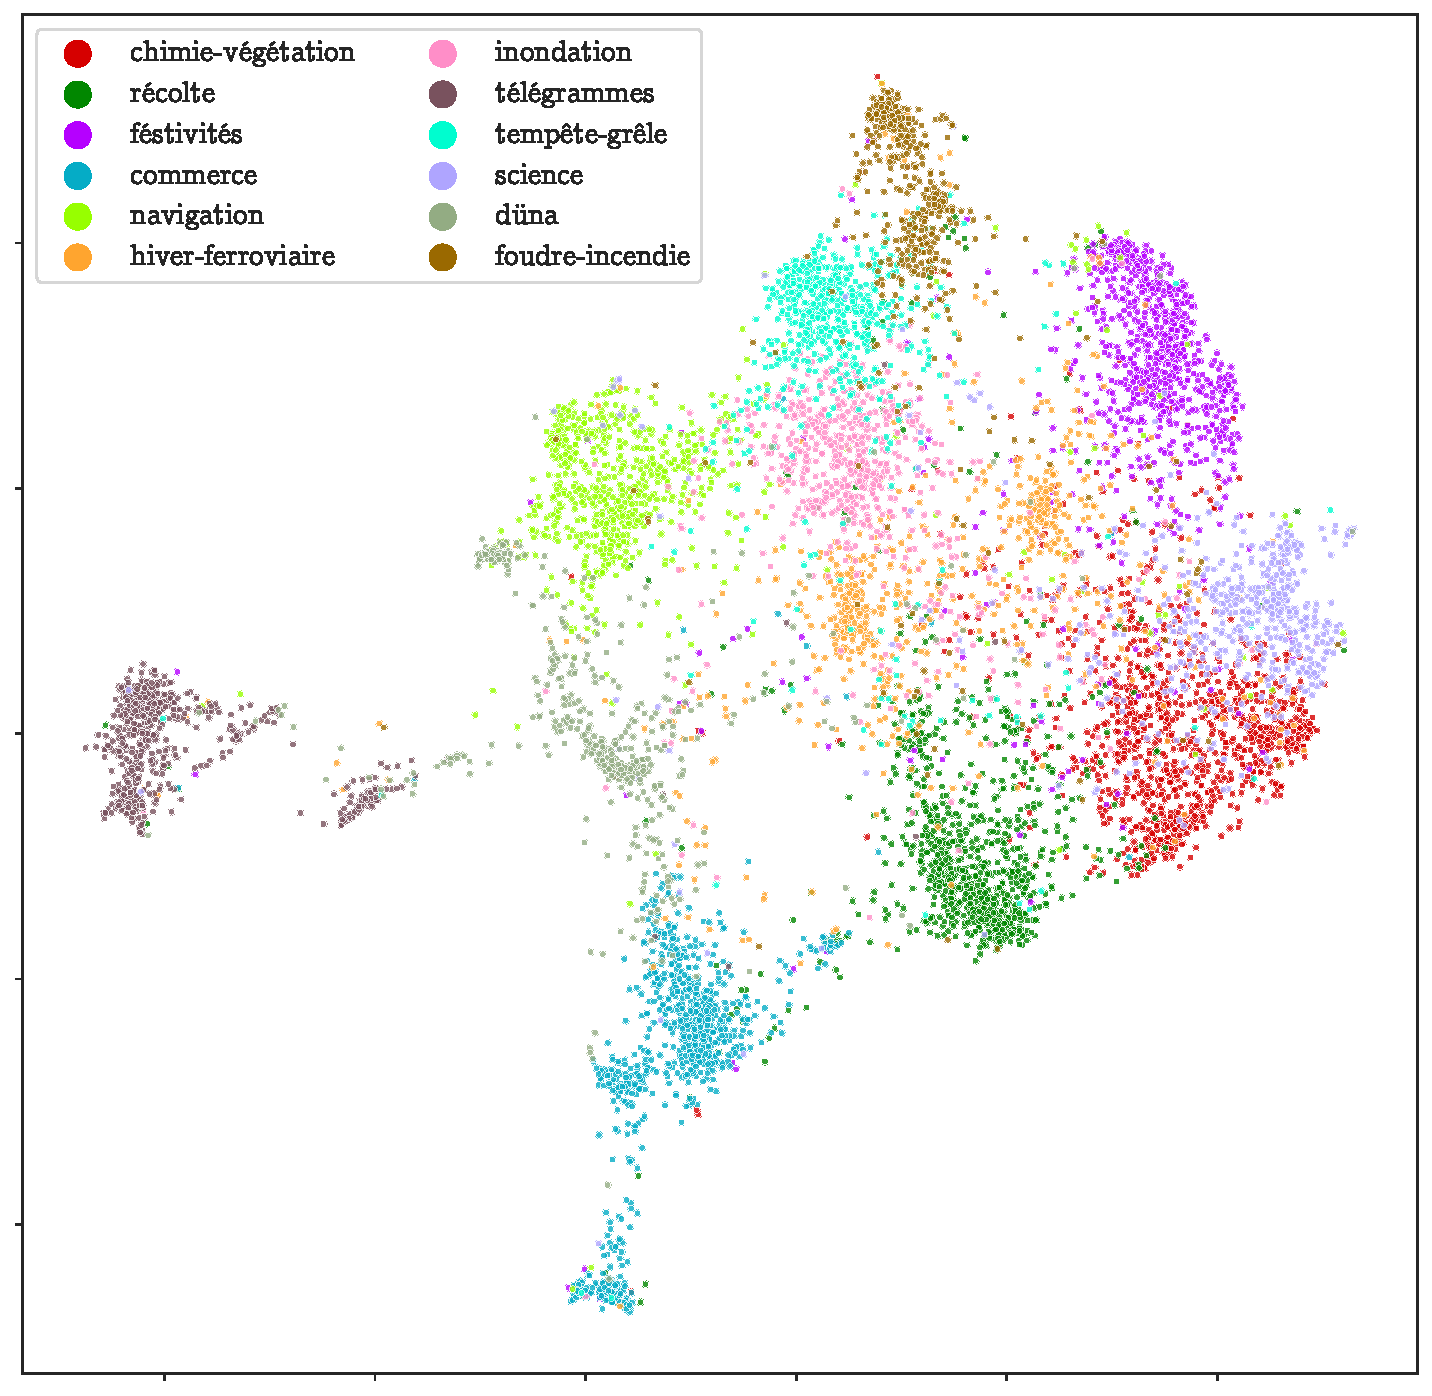
\includegraphics[width=\textwidth]{images/topics_umap.pdf}
    \caption{Visualisation spatiale des sujets}
    \label{fig:topic_umap}
\end{figure}

La visualisation ajoute une autre dimension à l'analyse thématique. Tout d'abord, on peut voir quels sont les sujets qui sont généralement les plus similaires les uns aux autres. Par exemple, les thèmes \textit{foudre-incendie}, \textit{tempête-grêle} et \textit{inondation} sont regroupés dans la partie supérieure de la figure. Tous ces thèmes contiennent principalement des descriptions d'événements singuliers et sont souvent de nature catastrophique, mentionnant des dommages et des victimes. La nature de ces sujets peut être encore mieux illustrée en examinant les 46 sujets originaux qui ont été fusionnés pour obtenir les sujets actuels. Par exemple, le sujet \textit{inondation} est compris de trois sujets originels, dont les mots caractéristiques sont montrés sur la figure \ref{fig:suptopic_worcloud_9}, où la taille des mots correspond à leur importance pour le sujet. Comme mentionné en haut, une partie du sujet \textit{inondation} est en fait compris des textes sur les avalanches (\textit{Lawine}), mais il est également intéressant de noter que le nuage au centre représente un sous-sujet des inondations en France (mots-clés \textit{Lyon}, \textit{Loire}, \textit{Rhône}, \textit{France} et \textit{Moniteur}). En examinant la répartition temporelle de ce sous-sujet, il s'avère que le plus grand nombre de ces textes-là proviennent des années 1846 et 1856, qui correspondent nettement aux graves inondations survenues en France ces années-là.\footcite{coeur_les_2004}

\begin{figure}[h]
    \centering
    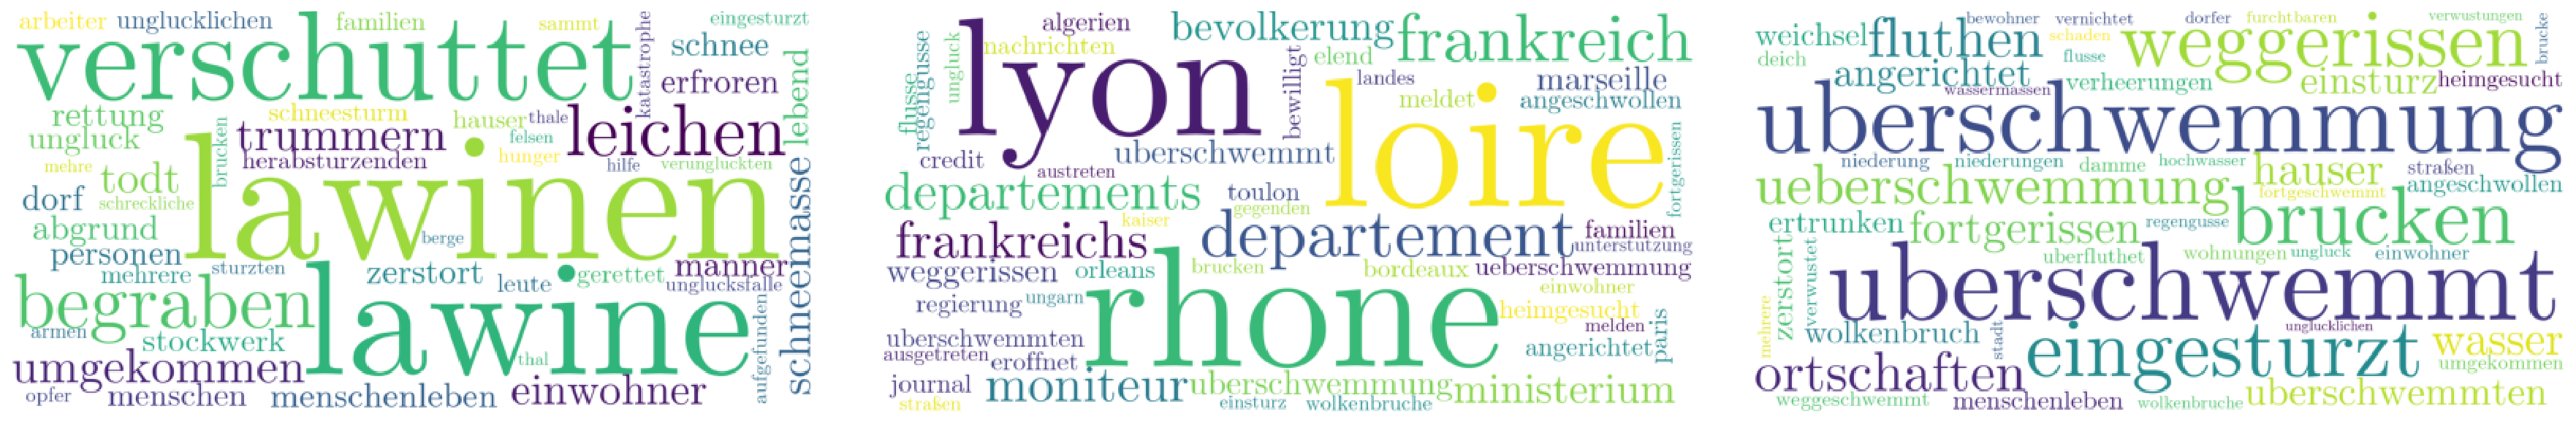
\includegraphics[width=0.9\textwidth]{images/subtopics_wordcloud_9.pdf}
    \caption{Nuages des mots des trois sujets qui composent le sujet \textit{inondation}}
    \label{fig:suptopic_worcloud_9}
\end{figure}


Dans la partie droite du graphique \ref{fig:topic_umap}, le thème \textit{chimie-végétation} présente un chevauchement important avec deux de ses voisins immédiats, \textit{science} et \textit{récolte}. En fait, de nombreux points dans cette zone de chevauchement appartiennent très probablement à deux thèmes dans une mesure presque égale, mais sont colorés par celui qui est légèrement dominant. Cela montre une transition assez douce entre les descriptions scientifiques du climat, truffées d'observations et autres, et les rapports agricoles sur les récoltes, par exemple. Parmi les documents qui comblent ce fossé, on pourrait probablement trouver de nombreux textes similaires à l'exemple 1 présenté à la page \pageref{topic1_chimie-vegetation} - une sorte de genre agricole-économique à l'esprit progressiste dont les prédécesseurs peuvent être trouvés dans la région balte et dans le reste de l'Europe à partir du XVII\textsuperscript{e} siècle.

\begin{figure}[h]
    \centering
    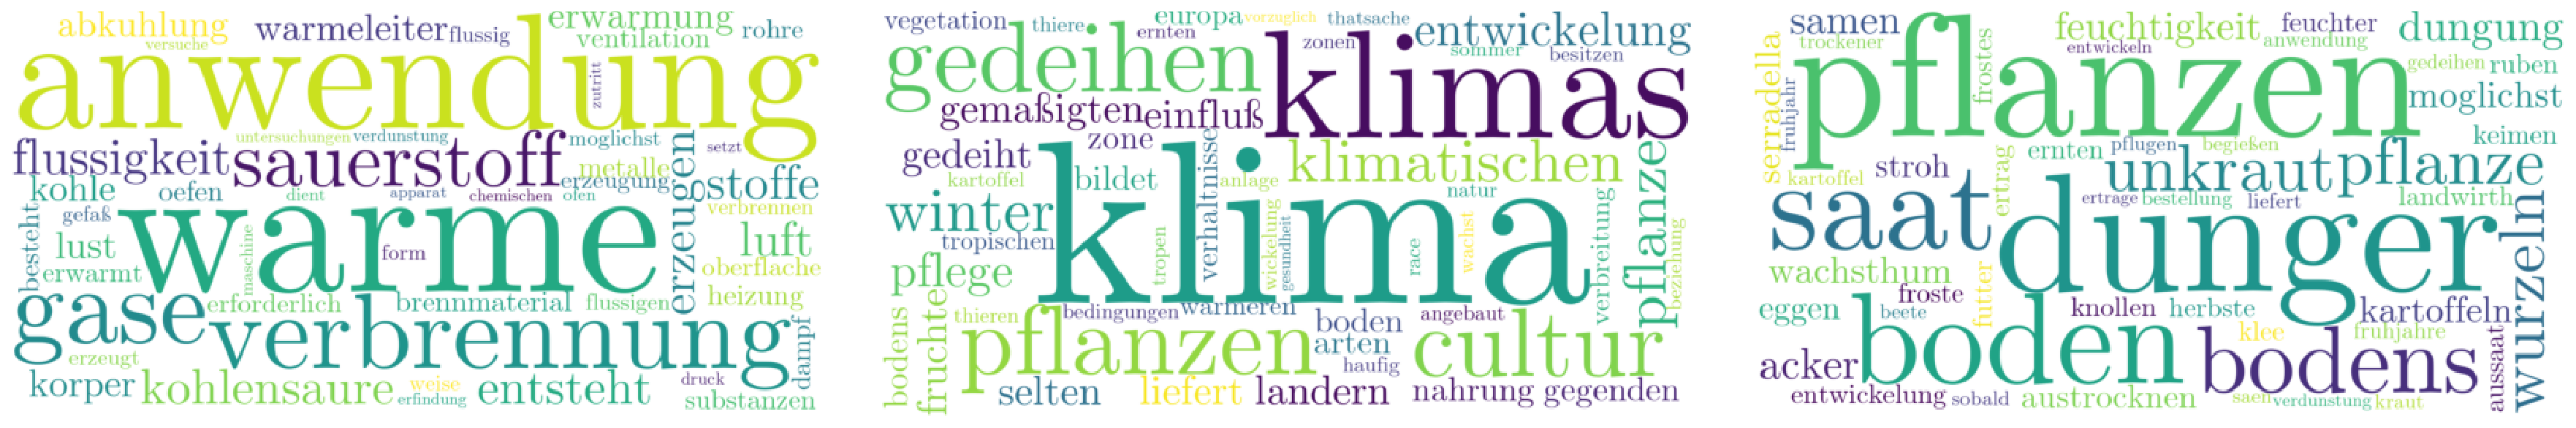
\includegraphics[width=0.9\textwidth]{images/subtopics_wordcloud_1.pdf}
    \caption{Nuages des mots des trois sujets qui composent le sujet \textit{chimie-végétation}}
    \label{fig:suptopic_worcloud_1}
\end{figure}

Ici aussi, il convient de jeter un coup d'œil aux sujets sous-jacents. La figure \ref{fig:suptopic_worcloud_1} montre les trois sujets originaux qui composent le sujet chimie-végétation. Le nuage sur la gauche est caractérisé par des mots comme \textit{application}, \textit{combustion}, \textit{oxygène}, \textit{liquide} - ces sont des textes scientifiques sur la chimie. Au centre, on trouve les mots \textit{liquide}, \textit{climat}, \textit{prospérité}, \textit{développement} et \textit{culture}, qui sont des indices du discours des sciences naturelles, possiblement dans un sens appliqué ou vulgarisé. Enfin, le nuage sur la droite exemplifie le côté agricole-économique du sujet, avec des mots comme \textit{plantes}, \textit{semis}, \textit{engrais}, \textit{sol}, \textit{mauvaises herbes}. Comme expliqué à la page \pageref{46_topics}, le nombre réduit de sujets (d'abord 16, puis 12 après l'élimination des 4 sujets faux-positifs) a été choisi selon l'interprétabilité générale de tous ces sujets, mais il est difficile à arriver à des distinctions parfaites pour tous les sujets.

Les sujets \textit{télégrammes} et \textit{commerce} sont éloignés et plutôt isolés des autres types de textes. Comme expliqué aux pages \pageref{topic10_télégrammes} et \pageref{topic4_commerce}, cela est très probablement dû à leur format rigide, les informations météorologiques apparaissant dans un contexte très spécifique. Comme le montrent les figures des pages \pageref{topic10_télégrammes} et \pageref{topic4_commerce}, ces thèmes sont également très clairement délimités dans le temps, faisant partie d'articles publiés régulièrement, mais sur une période relativement courte. Alors que \textit{télégrammes} est presque complètement isolé des autres thèmes, \textit{commerce} est lié à eux par \textit{düna}. Cela n'est pas surprenant, étant donné que ces documents sont également assez routiniers (mais pas autant que \textit{télégrammes} ou \textit{commerce}). Le sujet \textit{navigation} se positionne entre \textit{düna} et \textit{inondation}, ce qui est également logique car il s'agit souvent des descriptions détaillées comme c'est aussi le cas pour le groupe \textit{inondation}-\textit{tempête-grêle}-\textit{foudre-incendie}, mais certaines thèmes ne sont pas trop éloignées de ceux de \textit{Düna} (les deux sont connectés à l'eau et le transport maritime).

Parmi tous les sujets, \textit{hiver-ferroviaire} semble être le plus flou. Ses sous-sujets ne montrent pas une distinction claire qui pourrait expliquer ce fait. Les causes de la relative incohérence de ce thème méritent une analyse plus approfondie, mais il est possible qu'elle soit principalement due à la forte connexion entre ce thème et le mot-clé \textit{neige}, ce qui pourrait conduire à classer de nombreux textes relatifs à l'hiver comme appartenant à ce thème, indépendamment de leurs différents contextes.

\begin{figure}[h]
    \centering
    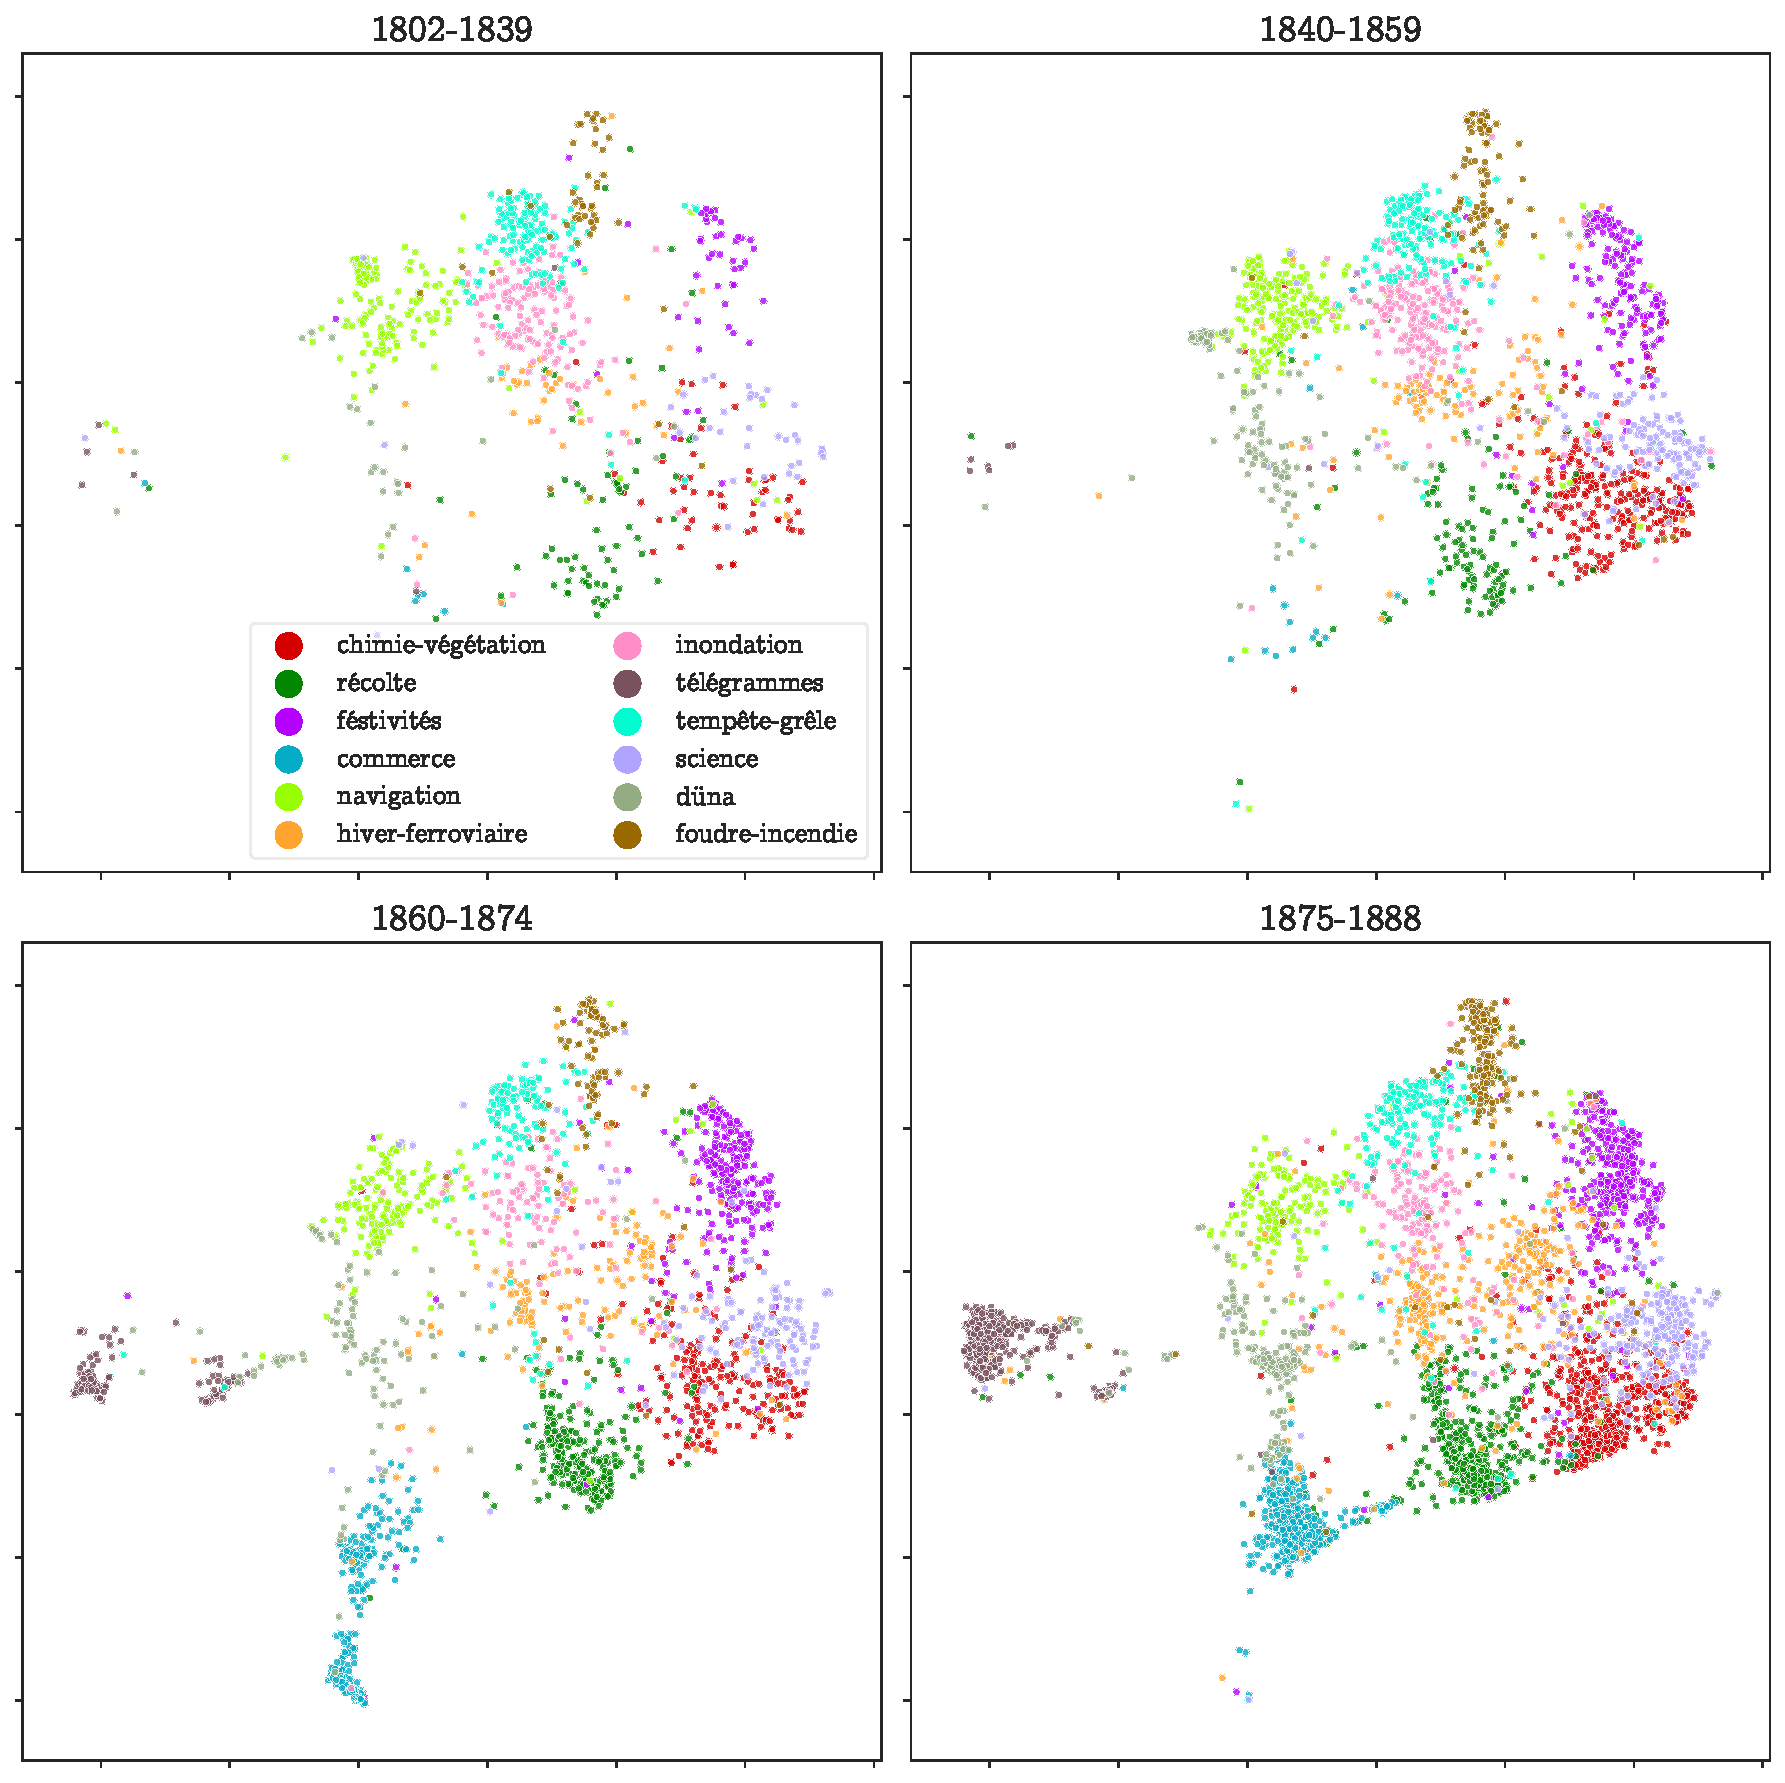
\includegraphics[width=\textwidth]{images/topics_umap_periods.pdf}
    \caption{Visualisation spatiale des sujets, divisée en quatre périodes}
    \label{fig:topics_umap_periods}
\end{figure}

Une autre possibilité d'analyse consiste à intégrer la dimension temporelle. La figure \ref{fig:topics_umap_periods} montre une projection UMAP de tous les segments, mais divise la plage temporelle en quatre périodes. Pour chaque fenêtre, seuls les segments qui ont été publiés pendant la période correspondante sont présentés.\footnote{Le positionnement des points sur ces graphiques peut légèrement différer de celui de la figure \ref{fig:topic_umap}, en raison de deux exécutions distinctes de l'algorithme UMAP.} Les périodes ont été choisies pour refléter au mieux les changements thématiques, ainsi que pour compenser le déséquilibre temporel des données, la majorité des textes étant issus des dernières décennies de la période d'observation.

La vue temporelle montre approximativement quand les différents sujets ont commencé à se former. Par exemple, on peut constater que les sujets \textit{tempête-grêle}, \textit{navigation} et \textit{inondation} sont les plus constants tout au long du siècle. On pourrait même dire que les nuages correspondants sont les plus cohérents pendant la période 1840-1859 et non dans les périodes ultérieures, malgré l'augmentation des données. Quatre autres thèmes, à savoir \textit{festivités}, \textit{science}, \textit{chimie-végétation} et \textit{récolte}, ont quelques occurrences entre 1802 et 1839, mais se forment beaucoup plus clairement dans la période 1840-1859. A partir de 1860, nous pouvons voir l'apparition soudaine de deux autres sujets, \textit{télégrammes} et \textit{commerce} - ceci correspond à l'analyse des sections précédentes. Le sujet \textit{düna}, par contre, est déjà visible entre 1840 et 1859. Enfin, la formation de \textit{hiver-ferroviaire} est à nouveau la plus floue, le nombre de points augmentant régulièrement à chaque période mais ne formant jamais un nuage aussi cohérent que les autres.

%\begin{figure}[h]
%    \centering
%    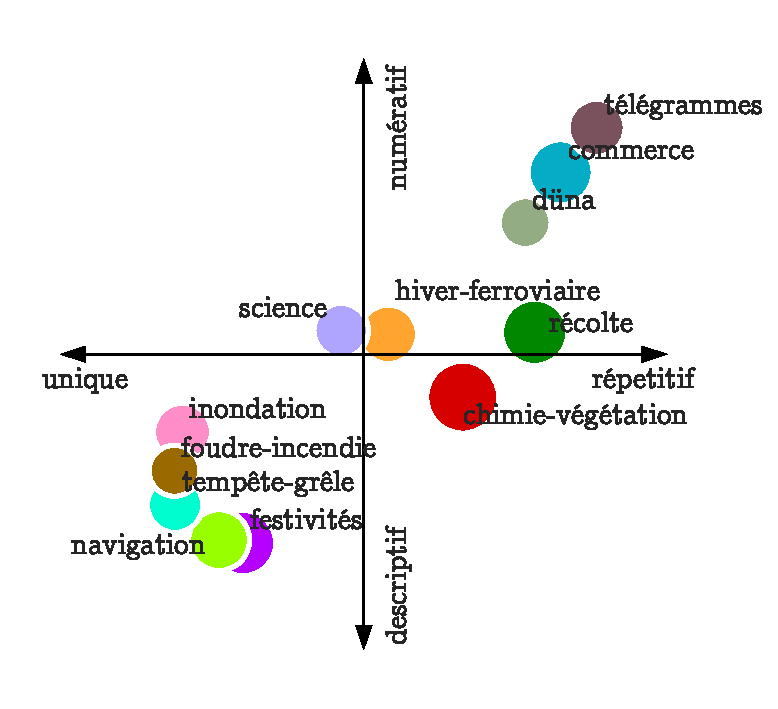
\includegraphics[width=0.7\textwidth]{im%ages/conceptual_scatterplot.pdf}
%    \caption{Comparaison conceptuelle des %sujets}
%    \label{fig:conceptual_scatterplot}
%\end{figure}

En tenant compte de la catégorisation des sources de l'histoire du climat proposée par Christian Pfister, il me semble raisonnable de considérer l'ensemble des sujets sur deux axes théoriques, \og personnel-institutionnel \fg{} et \og descriptif-instrumental \fg{}. \og Descriptif \fg{} peut être compris ici comme correspondant à la catégorie \og direct \fg{} du tableau \ref{tab:source_types}. La raison de ce changement est que tous les segments utilisés ici pour la modélisation des sujets contiennent des mots-clés liés au climat, ce qui en fait déjà des sources \og directes \fg{} par opposition aux sources indirectes, où les indices sur le climat peuvent être dérivés d'autres types d'informations. En ce sens, les sujets qui penchent du côté \og descriptif \fg{} utilisent des mots pour relayer des informations sur le temps, tandis que ceux qui se trouvent du côté \og instrumental \fg{} s'appuient sur des chiffres. Les sujets qui se situent à l'extrémité \og personnelle \fg{} de l'échelle consistent en des textes écrits et communiqués par des individus, tandis que ceux qui penchent vers \og institutionnelle \fg{} sont compilés par des organismes officiels du gouvernement, des sociétés scientifiques, des administrations portuaires, etc.

La figure \ref{fig:conceptual_scatterplot} montre une manière possible de comparer les thèmes entre eux sur ces échelles conceptuelles. La taille des cercles correspond au nombre de segments pour chaque sujet, mais leur positionnement est plutôt intuitif. La figure essaie de résumer les différences les plus fondamentales entre tous les sujets décrits et leur rôle dans la presse.

\begin{wrapfigure}{r}{0.6\textwidth}
  \begin{center}
    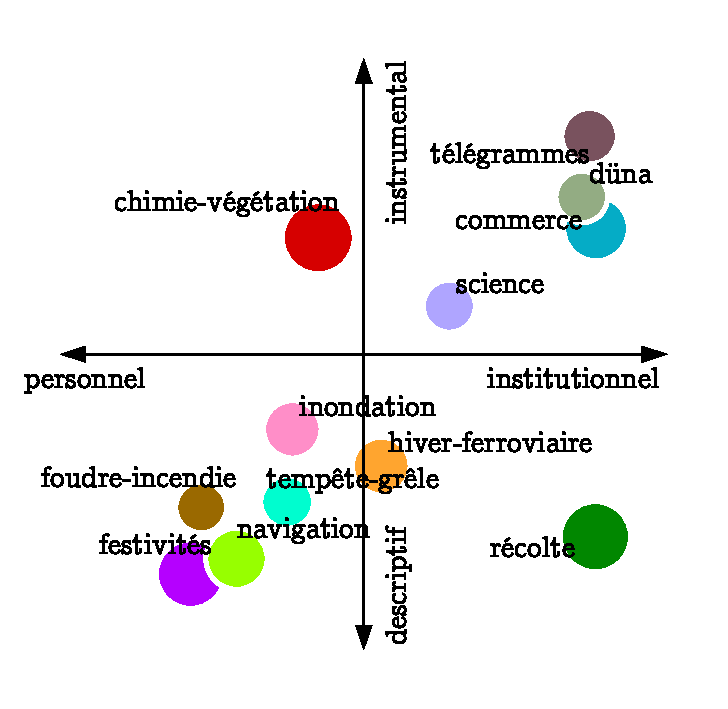
\includegraphics[width=0.6\textwidth, frame]{images/conceptual_scatterplot2.pdf}
  \end{center}
  \vspace*{-2ex}
  \captionsetup{justification=centering}
  \caption{Comparaison conceptuelle des sujets}
  \label{fig:conceptual_scatterplot}
\end{wrapfigure}

Plus précisément, la figure aide à préciser le rôle de la presse comme source d'histoire du climat, en répondant à la question \og en quoi les informations sur le climat et sur le temps constituent-elles des nouvelles ? \fg{} En tenant compte de l'analyse de ce chapitre, on peut dire que dans les premières décennies du XIX\textsuperscript{e} siècle, les informations météorologiques ont principalement trouvé leur chemin vers la presse sous la forme d'événements spécifiques qui ont été rapportés par des personnes individuelles, par exemple des correspondants. Une partie notable de ces informations concernait à son tour des événements extrêmes qui avaient souvent des effets socio-économiques négatifs (\textit{foudre-incendie}, \textit{tempête-grêle}, \textit{inondation}, \textit{navigation}). Dans ces textes, le climat pouvait être considéré comme le sujet des événements : toujours présent lors des célébrations et des rassemblements, même sans invitation ; capable de ruiner les récoltes et de couler les navires sur son caprice. Peu à peu, cependant, une autre vision du climat s'est imposée dans la presse. C'est l'apparition de textes scientifiques, botaniques et agro-économiques qui pensent au climat de manière abstraite - non pas comme des événements uniques mais comme un élément sous-jacent du monde physique qu'il faut étudier et exposer (exprimés par les sujets \textit{science} et \textit{chimie-végétation}). Enfin, dans la seconde partie du siècle et surtout à partir des années 1860, la presse commence à rendre compte du climat de manière systématique et répétitive. Le climat s'est ainsi intégré à d'autres informations comme les cours de la bourse, les horaires de train et les rapports de navigation (\textit{commerce}, \textit{düna}, \textit{télégrammes}). Ces trois modes de présentation de l'information - narrations des événements uniques, descriptions scientifiques et rapports systématiques - ne se sont pas substitués les uns aux autres mais ont plutôt existé en parallèle.

Il est intéressant de comparer ces développements aux conclusions de Jan Golinski sur le rôle de la météo dans la société (voir la page \pageref{golinski}). Tout d'abord, il est évident que la presse a eu un intérêt constant et considérable pour le temps au cours du XIX\textsuperscript{e} siècle. Les événements météorologiques extrêmes (comme les inondations ou les tempêtes) attiraient l'attention du public et étaient souvent rapportés de manière très détaillée, car ils constituaient une catégorie pure de \og nouvelles \fg{}, grâce à leur imprévisibilité. Nous pouvons constater que ces types de nouvelles constituent le type d'informations météorologiques le plus persistant dans la presse pendant toute la période d'observation. D'autre part, Golinski parle également de changements dans la représentation de la météo, et les résultats présentés ici soutiennent ses idées. Nous pouvons observer que les sujets qui commencent à apparaître au milieu du siècle et surtout à partir des années 1860 - \textit{düna}, \textit{commerce} et \textit{télégrammes} - sont différents des types de textes précédents. Ils sont tous publiés régulièrement, que ce soit en cas ou en l'absence de temps \og digne d'intérêt \fg{}. Ils intègrent également des observations répétitives (à la fois numériques et descriptives), comme la température, la vitesse du vent ou le niveau de l'eau. 

Au chapitre \ref{contenu}, la rubrique \textit{Witterungsbeobachtungen in Riga} (observations météorologiques à Riga) a été mentionnée. Comme décrit à la page \pageref{beobachtungen_riga}, les articles portant ce titre ont été écartés avant toute analyse ultérieure car leur contenu était presque entièrement numérique et contenait la plus grande proportion d'erreurs d'OCR, ce qui les rendait inadaptés aux méthodes utilisées dans ce mémoire. Cependant, il est intéressant de noter que la plage temporelle de cette rubrique coïncide avec l'apparition des sujets \textit{commerce} et \textit{télégrammes}. Par conséquent, elle pourrait également être considérée comme un sujet à part entière, étant donné que son contenu peut être déterminé même sans modélisation du sujet. Cela donne du poids à l'affirmation selon laquelle le temps est représenté d'une manière nouvelle et plus répétitive à partir des années 1860, ou \og rendu quotidien \fg{}, comme le dit Golinski.\footcite[18]{golinski_time_2003}



\clearpage

\section*{Conclusion}
\addcontentsline{toc}{section}{Conclusion}

Le premier axe de recherche de ce mémoire était d'expérimenter des méthodes numériques pour extraire des informations utiles à l'histoire du climat. L'étude s'est basée sur près de 300 000 articles de journaux numérisés de la publication \textit{Rigasche Zeitung}, couvrant la période 1802-1888. Cet ensemble spécifique de sources avait ses propres avantages et limites. La qualité de l'OCR et de la segmentation était raisonnablement bonne, ce qui a permis d'approcher la majorité des données même avec des méthodes numériques avancées. Cependant, une certaine partie des données a été jugée illisible et a dû être écartée. Les métadonnées suffisantes, notamment la présence de titres d'articles, ont constitué un avantage certain, car elles ont permis de faire des généralisations sur l'évolution de la structure du journal et sur les principaux sujets abordés. Cela a également permis de nuancer l'analyse de la présence d'informations météorologiques.

Après le prétraitement et la tokenisation des données, les informations météorologiques contenues dans les sources ont d'abord été analysées au niveau des mots. Après une tentative insatisfaisante d'apprentissage supervisé, décrite dans la section \ref{NER_approach}, une approche basée sur le corpus a été adaptée. Celle-ci s'est avérée beaucoup plus robuste, grâce au volume des données. Les vecteurs de mots calculés à partir du corpus se sont avérés très efficaces pour capturer les qualités sémantiques des tokens.

Dans la section \ref{distributional_semantics_approach}, une approche originale pour faire converger les variations orthographiques et grammaticales a été mise en œuvre. Elle consistait à utiliser la similarité vectorielle pour capturer les formes alternatives qui existent dans le corpus, soit en raison d'erreurs d'OCR, soit en raison de variations grammaticales et orthographiques historiques. Cette méthode s'est avérée très efficace : avec elle, un ensemble initial de 42 mots a été élargi à plus de 300 schémas exprimant des significations similaires. Cette méthode pourrait présenter un intérêt plus large pour le domaine des humanités numériques, car son utilisation ne se limite pas à l'histoire du climat. Avec des recherches supplémentaires, elle pourrait être développée en une méthode plus systématisée pour contourner les variations de l'OCR dans les sources numérisées, un problème persistant pour de nombreuses approches computationnelles.

La section \ref{entity_distribution} a examiné les différentes possibilités d'utilisation des fréquences de tokens et leurs contextes immédiats pour trouver des informations climatiques dans les données. Dans un premier temps, la comparaison des fréquences globales des mots-clés donne un aperçu des phénomènes météorologiques les plus représentés dans la presse. Dans un deuxième temps, les visualisations temporelles des fréquences de mots clés peuvent faire ressortir des pics qui peuvent ensuite être analysés plus en détail pour trouver leurs causes. Ce type de traçage peut conduire à la détection d'événements météorologiques concrets - ce qui peut être très utile pour les historiens du climat qui recherchent un type spécifique de phénomènes météorologiques.

Il y a cependant plusieurs choses à garder à l'esprit lors de la recherche de pics dans la fréquence des mots-clés. Premièrement, le nombre de mentions d'un phénomène climatique ne dit bien sûr rien sur la fréquence réelle de ce phénomène dans le monde réel. Il s'agit plutôt d'un intérêt accru de la presse (ou de la société, par extension) qui peut être causé par de multiples facteurs et nécessite donc une bonne connaissance des sources et de leur contexte. Deuxièmement, dans certains cas, le mot-clé d'intérêt ne signifie pas du tout un phénomène météorologique. Pour contrer cela, l'analyse du contexte immédiat des mots-clés a également été explorée. Bien qu'elle ne soit pas aussi efficace que la modélisation thématique, elle peut donner des informations précieuses sur les représentations de phénomènes météorologiques spécifiques - quelque chose qui est également d'une utilité potentielle pour l'historien du climat.

Le chapitre \ref{topic_modeling} de ce mémoire a été consacré à la modélisation thématique de'environ 12 000 segments de texte du journal contenant un nombre suffisant de mots-clés liés au climat. La méthode choisie, \textit{top2vec}, a identifié un certain nombre de thèmes relativement bien interprétables dans les textes. Cela a permis d'organiser les informations météorologiques et climatiques en catégories qui pourraient ensuite être analysées séparément. La comparaison de ces sujets sur le plan sémantique (en utilisant la similarité vectorielle), temporel et par leurs métadonnées (par exemple les titres d'articles) a révélé une image intéressante du discours sur le climat dans la presse du XIX\textsuperscript{e} siècle tel qu'il se trouve dans le \textit{Rigasche Zeitung}. La capacité de l'algorithme \textit{top2vec} à fusionner des sujets similaires les uns dans les autres s'est avérée très utile. en permettant au chercheur de choisir un niveau de généralisation préféré, mais aussi de se référer aux plus petits groupes de textes qui composent des sujets plus vastes. La modélisation de sujets peut également servir de méthode pour éliminer les mentions fausses-positives de la météo, par exemple les utilisations métaphoriques et littéraires. Cela peut potentiellement être utilisé pour compléter une analyse basée sur des mots clés.

La modélisation de sujets aide également à préciser le rôle des journaux en tant que source d'histoire du climat et nuancer les conclusions des études existantes. Les résultats montrent que les journaux peuvent englober un très large éventail de types d'informations, des narrations de type chronique aux observations météorologiques de routine, ce qui souligne la valeur des journaux en tant que sources d'histoire du climat. Dans le contexte du XIX\textsuperscript{e} siècle, les journaux pourraient plutôt être considérés comme des points d'accès à tous les types de sources, leur variance augmentant régulièrement au fil du temps.

Cependant, la modélisation de sujets a aussi ses limites. Premièrement, tous les textes ne relèvent pas d'une seule catégorie et certains sujets peuvent être difficiles à généraliser. Se concentrer sur les textes les plus représentatifs donne une bonne idée des sujets dans leur forme la plus pure, mais dans certains cas, l'idée sous-jacente deviendra rapidement fluide au fur et à mesure que l'on commencera à prendre en compte les textes qui sont moins centraux au sujet. Le fait que \textit{top2vec} permette aux textes d'appartenir à plusieurs sujets ouvre des possibilités mais rend également difficile la quantification fiable de la taille de ces sujets.

Les méthodes utilisées dans ce mémoire peuvent potentiellement aussi être appliquées à d'autres sources dans le futur. À l'heure actuelle, les implémentations sont centrées sur le format spécifique du corpus LNB, mais elles peuvent être adaptées à d'autres corpus de sources de journaux. Par exemple, il serait intéressant de comparer les résultats sur le \textit{Rigasche Zeitung} à ceux d'autres journaux de langue allemande de la même période. En incorporant plus de données, les méthodes présentées ici pourraient être développées davantage pour recueillir de grandes quantités de données sur le climat historique, en particulier dans les régions où les données d'observation standardisées sont rares. Même lorsqu'il était publié dans la semi-périphérie de l'Europe du XIX\textsuperscript{e} siècle, le \textit{Rigasche Zeitung} faisait clairement partie de la circulation générale des nouvelles européennes, et plus particulièrement de la partie germanophone de l'Europe. Ceci est très important, car sinon, les résultats présentés ici auraient une valeur de généralisation moindre, même si les méthodes numériques utilisées sont largement indépendantes de la langue. À l'heure actuelle, cependant, les approches utilisées ici peuvent être adaptées à d'autres sources de même type avec une relative facilité, et l'interconnexion du réseau de presse du XIX\textsuperscript{e} siècle nous encourage à considérer que les résultats représentent plus que le contenu d'un seul journal.

Le deuxième axe de recherche concerne la relation de la société avec le temps et le climat, telle qu'elle apparaît dans les sources. Dans ses limites actuelles, le mémoire ne fait que des pas exploratoires vers de telles conclusions, car il faudrait beaucoup plus de temps pour parvenir à une meilleure compréhension d'un sujet aussi vaste. Néanmoins, le processus de recherche a mis en évidence plusieurs détails intéressants qui peuvent être développés et comparés à d'autres études. Tout d'abord, la météo semble être un sujet d'actualité relativement stable sur l'ensemble de la période - aucun changement évident de sa popularité ne peut être noté sur le long terme. Les informations sur le temps sont dominées par un petit nombre de mots-clés généraux - tempêtes, vent, pluie, temps, neige, froid etc. ; il s'agit de phénomènes courants mais qui ont une importance quotidienne dans la vie des gens.

Deuxièmement, les sujets identifiés au chapitre \ref{topic_modeling} reflètent les différentes modalités d'interaction avec le temps. Certains sujets concernent des informations sur des accidents naturels (tempêtes de grêle, foudre et inondations). Il s'agit généralement de textes narratifs qui ne contiennent aucune donnée d'observation, mais qui peuvent souvent être très détaillés dans leur description des événements. Les naufrages et les rapports sur les événements publics présentent également un caractère similaire. Ce type d'informations météorologiques est le plus persistant tout au long du siècle.

Une deuxième catégorie d'informations liées au temps et au climat est plus analytique : les rapports scientifiques et les instructions agricoles. Par rapport à la première catégorie, ces textes abordent le temps de manière neutre, cherchant à l'expliquer - et à en tirer profit. Ils utilisent également des termes plus généraux, se référant davantage au climat, au temps et à leurs qualités générales qu'à des phénomènes ou événements spécifiques. Enfin, une troisième catégorie d'informations météorologiques consiste en des rapports de routine qui contiennent souvent des mesures d'une certaine nature. On les trouve à l'intérieur de rapports de navigation ou commerciaux, mais aussi explicitement sous la forme de télégrammes météorologiques et d'observations quotidiennes.

Il est intéressant de noter que les deuxième et troisième groupes de sujets n'apparaissent qu'au milieu du siècle. Les textes scientifiques, chimiques et botaniques ont commencé à faire plus d'apparitions après que le \textit{Rigasche Zeitung} soit devenu un journal quotidien dans les années 1840. Cela semble coïncider avec une diversification plus générale du contenu du journal (illustré dans la figure \ref{fig:headings_places}). Le troisième groupe de sujets, les rapports systématisés, commence à apparaître encore plus tard. En comparant les occurrences de ce type d'information, il semble qu'il soit lié aux développements de la communication et des transports, notamment la construction de chemins de fer et de lignes télégraphiques. La relation entre les progrès de la communication et la compréhension du temps par la société offre de riches possibilités de recherches futures, et plusieurs d'entre elles sont indiquées par les résultats de ce mémoire. L'augmentation de la vitesse de l'information et des transports semble avoir rendu le public plus intéressé par le temps qu'il fait dans des régions éloignées ; non seulement dans le cas de catastrophes et de phénomènes rares, les descriptions étaient consommées comme des nouvelles, mais aussi en absence de toute irrégularité.

Cette évolution n'est pas sans rappeler l'intérêt des individus de classes supérieures pour la tenue d'un journal météorologique et l'enregistrement des observations quotidiennes, mais dans ce cas, elle semble se produire à une échelle beaucoup plus grande, tant sur le plan social que spatial. Il semble que le temps ne soit pas seulement rendu quotidien, mais que son intégration dans les affaires courantes témoigne d'une volonté de le systématiser, voire de le contrôler. La météo dans ces rapports est dérivée de la subjectivité qui caractérise les rapports de tempête, par exemple. Elle fait également partie de l'État, comme en témoignent les télégrammes météorologiques qui communiquaient quotidiennement les températures et la pression atmosphérique de différentes villes de l'Empire russe. Cela s'apparente à la construction d'un \og climat national \fg{} décrit par Golinski, mais cette fois avec des technologies modernes et à plus grande échelle.

Il serait également intéressant de développer ici les résultats préliminaires et de les relier au monde contemporain. Au cours de la dernière semaine de rédaction de ce mémoire, j'ai rencontré plusieurs nouvelles concernant la météo qui présentaient une grande similitude avec celles sur lesquelles je faisais des recherches. D'énormes inondations au Pakistan ont laissé des dizaines de milliers de sans-abri, tandis qu'une étrange tempête de grêle avec des pierres plus grosses que des balles de tennis a frappé la Catalogne, faisant une victime. La nature de ces descriptions n'est pas du tout différente des rapports qui existaient dans les journaux au début du XIX\textsuperscript{e} siècle et déjà avant. Notre discours public actuel sur le climat semble avoir des racines profondes qui remontent au début de la modernité et au-delà. Des recherches plus approfondies sur ces thèmes pourraient donc, espérons-le, nous éclairer sur la manière dont nous lisons le climat à l'ère du réchauffement climatique.


\clearpage


\section*{Annexe A : Sujets du climat} \label{annexe}
\addcontentsline{toc}{section}{Annexe A : Sujets du climat}

\subsection*{Chimie-végétation} \label{topic1_chimie-vegetation}
\addcontentsline{toc}{subsection}{Chimie-végétation}

\begin{figure}[H]
\centering
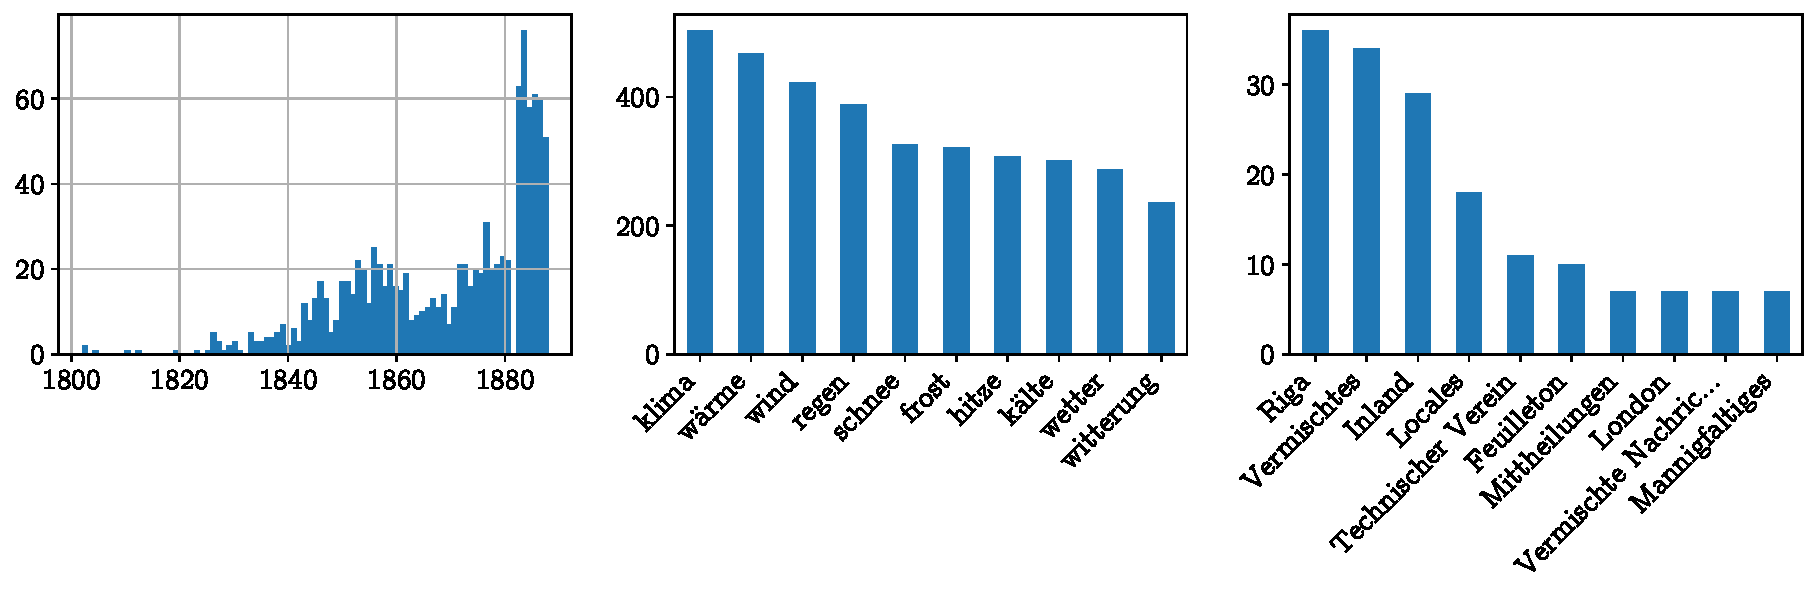
\includegraphics[width=\textwidth]{images/topic_charts_1.pdf}
\end{figure}

\begin{flushleft}
\textbf{Taille :} 1053 segments

\textbf{Mots caractéristiques :} \texttt{pflanzen}, \texttt{klima}, \texttt{pflanze}, \texttt{bodens}, \texttt{boden}, \texttt{moglichst}, \texttt{warme}, \texttt{anwendung}, \texttt{dunger}, \texttt{feuchtigkeit}, \texttt{oberflache}, \texttt{beziehung}, \texttt{winter}, \texttt{weise}, \texttt{giebt}, \texttt{besteht}, \texttt{gewohnlich}, \texttt{entwickelung}, \texttt{bildet}, \texttt{liefert}, \texttt{anlage}, \texttt{stoffe}, \texttt{ausgesetzt}, \texttt{erwarmung}, \texttt{regel}, \texttt{saat}, \texttt{erforderlich}, \texttt{verdunstung}, \texttt{falle}, \texttt{wurzeln}.
\end{flushleft}

\medskip

\noindent \textbf{Exemple 1 :} \og Il faut compter environ trois à quatre semaines, selon la variété de pomme de terre et les conditions météorologiques, avant que les plantes ne sortent de terre. Pendant ce temps, les conditions météorologiques, les mauvaises herbes, etc. peuvent déjà endommager les plantes ou du moins influencer leur croissance. \fg{}\footnote{\textit{Etwa drei bis vier Wochen, je nach der Kartoffelsorte und nach der Witterung, vergehen, bis die Pflanzen aus der Erde kommen. In dieser Zwischenzeit können aber Witterung, Unkräuter c. den Pflanzen schon Schaden zufügen oder wenigstens ihr Wachsthum beeinflussen.} RZ 11/06/1887 (\texttt{id: 282166})}

\noindent \textbf{Exemple 2 :} \og Seule la pratique et les différentes conditions locales peuvent déterminer s'il est indiqué, en toutes circonstances, de faire précéder la carbonisation de la sole sèche à l'air. La quantité importante d'eau hygroscopique contenue dans une telle tourbe (au moins 20\%) nécessite une dépense de combustible correspondante pour son évaporation lors de la carbonisation. Lorsque la chaleur nécessaire à la carbonisation est produite par la combustion d'une partie du matériau de carbonisation \fg{} [...].\footnote{\textit{Ob unter allen Umständen eine der Verkohlung vorausgehende Darrung der lufttrockenen Boden angezeigt ist, darüber können nur die Praxis und verschiedene Bedingungen localer Natur entscheiden. Die bedeutende Menge hygroskopischen Wassers, die ein solcher Torf enthält (mindestens 20 pCt.), erfordert zu ihrer Verdampfung bei der Verkohlung einen entsprechenden Auswand von Brennmaterial.} RZ 28/07/1877 (\texttt{id: 235631})}

\clearpage



\subsection*{Récolte} \label{topic2_recolte}
\addcontentsline{toc}{subsection}{Récolte}

\begin{figure}[H]
\centering
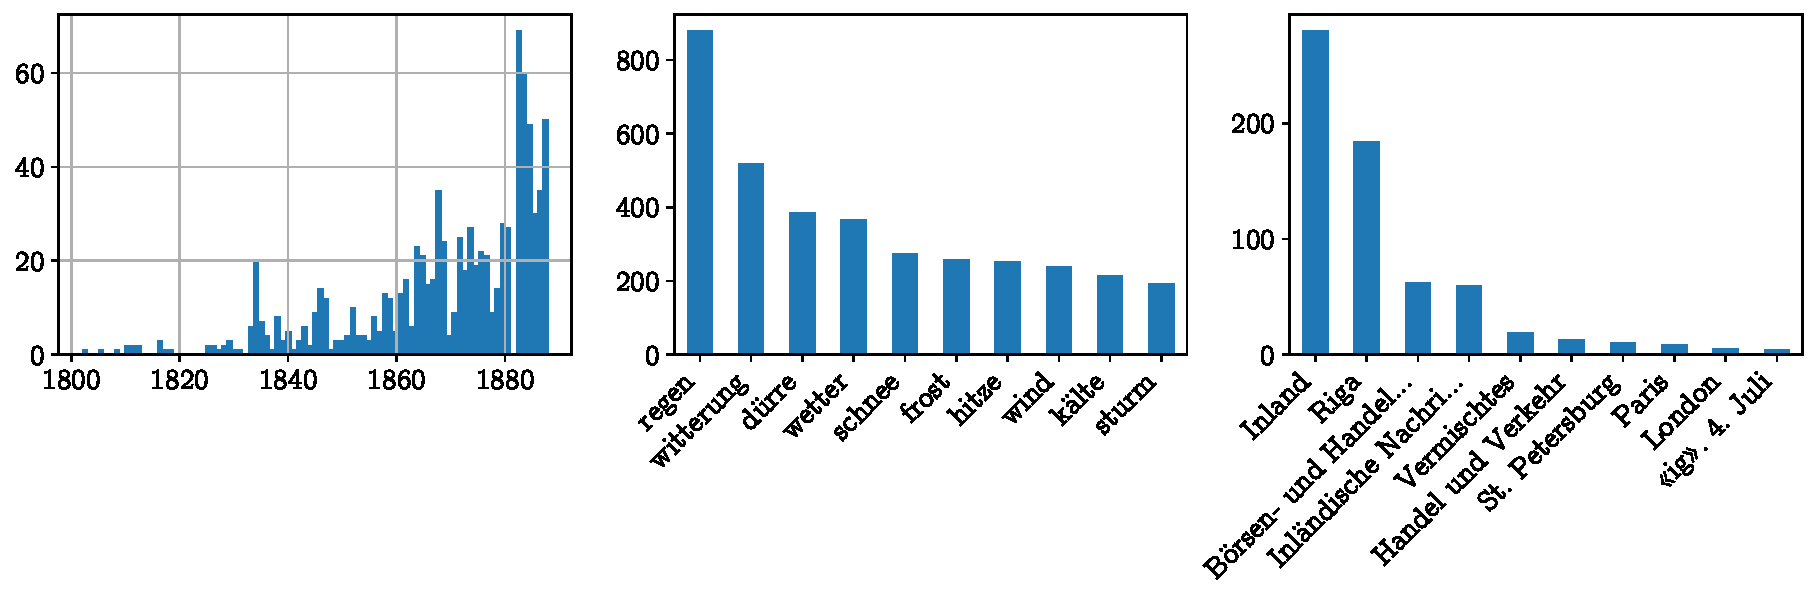
\includegraphics[width=\textwidth]{images/topic_charts_2.pdf}
\end{figure}

\begin{flushleft}
\textbf{Taille :} 887 segments

\textbf{Mots caractéristiques :} \texttt{ernte}, \texttt{durre}, \texttt{heuernte}, \texttt{ertrag}, \texttt{sommergetreide}, \texttt{mittelmaßige}, \texttt{sommerkorn}, \texttt{felder}, \texttt{wintergetreide}, \texttt{mittelmaßig}, \texttt{sommersaaten}, \texttt{korn}, \texttt{graswuchs}, \texttt{kreise}, \texttt{verspricht}, \texttt{saat}, \texttt{gelitten}, \texttt{wintersaaten}, \texttt{befriedigend}, \texttt{klee}, \texttt{wachsthum}, \texttt{aussaat}, \texttt{wintersaat}, \texttt{roggen}, \texttt{roggenernte}, \texttt{geschadet}, \texttt{saaten}, \texttt{kartoffeln}, \texttt{sommergetreides}, \texttt{winterfelder}.
\end{flushleft}

\medskip

\noindent \textbf{Exemple :} \og Estonie. En ce qui concerne l'état des champs et des prairies en Estonie, les rapports des juges des villages au comité de statistique pour la période du 7 juillet sont les suivants : la floraison du seigle s'est déroulée favorablement et l'état de celui-ci a été généralement satisfaisant, de sorte qu'à l'exception de Waiwara, Strandwierland et d'une partie de la Wiek, où l'aspect du grain a été moins satisfaisant, on peut s'attendre à une récolte plus que moyenne. Les céréales d'été et les pommes de terre, qui avaient souffert de la sécheresse d'avant la Saint-Jean, se sont généralement rétablies grâce aux pluies ultérieures. Dans la Wiek, on rapporte que les premières semences se sont flétries à cause de la sécheresse et que les dernières n'ont presque pas pu germer. La fauche du foin était en grande partie terminée et le résultat était toujours satisfaisant, tant en quantité qu'en qualité, et même excellent par endroits. On ne se plaignait nulle part de la grêle et des insectes nuisibles. \fg{} \footnote{\textit{Estland. Ueber den Stand der Felder und Wiesen in Estland lauten die Berichte der Hakenrichter an das statistische Comité für die Zeit des 7. Juli folgendermaßen: Die Blüthezeit
des Roggens war günstig verlaufen und der Stand desselben meist befriedigend, so daß mit Ausnahme von Waiwara, Strandwierland und von einem Theile der Wiek, wo das Aussehen des Korns weniger befriedigte, wohl auf eine mehr als mittelgute Ernte zu rechnen ist. Das Sommerkorn und die Kartoffeln, welche durch die vor Johannis
herrschende Dürre gelitten hatten, hatten sich im Allgemeinen in des später gefallenen Regens erholt. Aus der Wiek wird berichtet, daß die frühesten Saaten in Folge der Dürre welkten und daß die späteren fast gar nicht hatten keimen können. Die Heumahd war zum größten Theile
beendet und das Resultat derselben eine sowohl nach Quantität als Qualität durchgängig befriedigendes, stellenweise sogar vorzügliches. Ueber Hagelschläge und schädliche Insecten verlautete nirgends eine Klage.} RZ 25/08/1856 (\texttt{id: 269301})}


\subsection*{Festivités} \label{topic3_festivités}
\addcontentsline{toc}{subsection}{Festivités}

\begin{figure}[H]
\centering
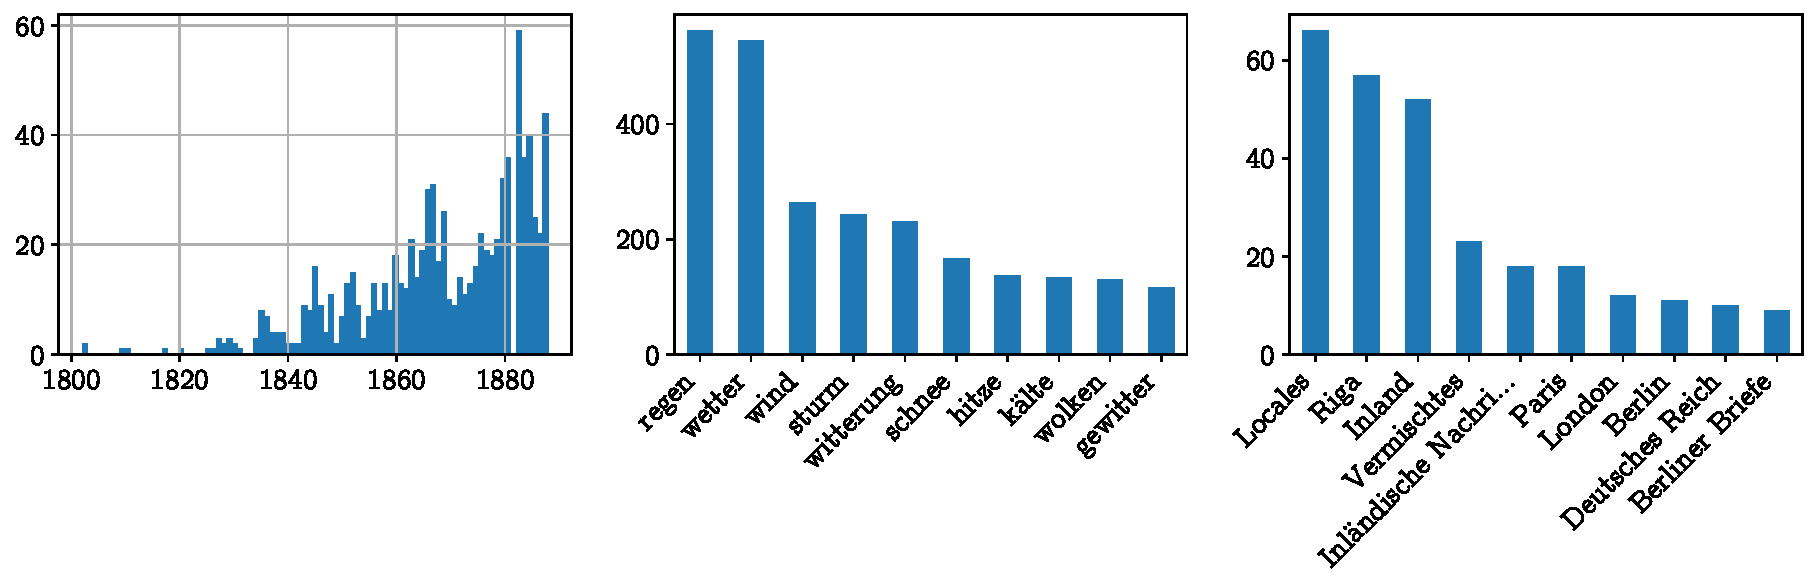
\includegraphics[width=\textwidth]{images/topic_charts_3.pdf}
\end{figure}

\begin{flushleft}
\textbf{Taille :} 858 segments

\textbf{Mots caractéristiques :} \texttt{publicum}, \texttt{musik}, \texttt{gaste}, \texttt{theater}, \texttt{trotz}, \texttt{herrn}, \texttt{sanger}, \texttt{feier}, \texttt{damen}, \texttt{beifall}, \texttt{publicums}, \texttt{concert}, \texttt{besuch}, \texttt{illumination}, \texttt{versammelt}, \texttt{genuß}, \texttt{schonen}, \texttt{besucht}, \texttt{locales}, \texttt{platz}, \texttt{festlich}, \texttt{feuerwerk}, \texttt{concerte}, \texttt{vergnugen}, \texttt{zuschauer}, \texttt{programm}, \texttt{capelle}, \texttt{eindruck}, \texttt{herren}, \texttt{saal}.
\end{flushleft}

\medskip

\noindent \textbf{Exemple :} \og Le jardin impérial a fait une triste expérience cet été. Si une entreprise quelconque y était annoncée, dont on pouvait espérer une plus grande affluence de visiteurs, on pouvait supposer avec quasi-certitude que cette soirée serait pluvieuse, et la pluie peut faire le désespoir des propriétaires d'établissements de jardin. Il est d'autant plus réjouissant que la pluie ait épargné hier soir les illuminations et les feux d'artifice organisés dans le jardin impérial. Un public assez nombreux s'était donc réuni hier sous les vieux arbres feuillus ombragés du jardin. Le feu d'artifice était très beau ; l'étang, dans lequel se reflétaient des centaines de lampions multicolores, offrait un spectacle encore plus beau.\fg{}\footnote{\textit{(Der Kaiserliche Garten) hat in diesem Sommer eine trübe Erfahrung machen müssen. War in demselben irgend ein Unternehmen angesagt, von dem stärkerer Zuspruch an Gästen sich erhoffen ließ, so konnte man mit ziemlicher Sicherheit annehmen, daß dieser Abend verregnete, und Regen kann die Inhaber von Gartenetablissements zur hellen Verzweiflung bringen. Um so erfreulicher, daß wenigstens gestern Abend der leidige Regen die im Kaiserlichen Garten veranstaltete Illumination nebst Feuerwerk mit seinem unerbetenen Dazwischenkommen verschonte. So hatte sich denn gestern auch ein recht zahlreiches Publicum unter den alten schattigen Laubbäumen des Gartens versammelt. Das Feuerwerk war recht nett; einen noch schöneren Anblick gewährte der Teich, in dem sich Hunderte von bunten Lampions in wechselndem Farbenspiel wiederspiegelten.} RZ 07/07/1888 (\texttt{id: 287414})}

\clearpage

\subsection*{Commerce} \label{topic4_commerce}
\addcontentsline{toc}{subsection}{Commerce}

\begin{figure}[H]
\centering
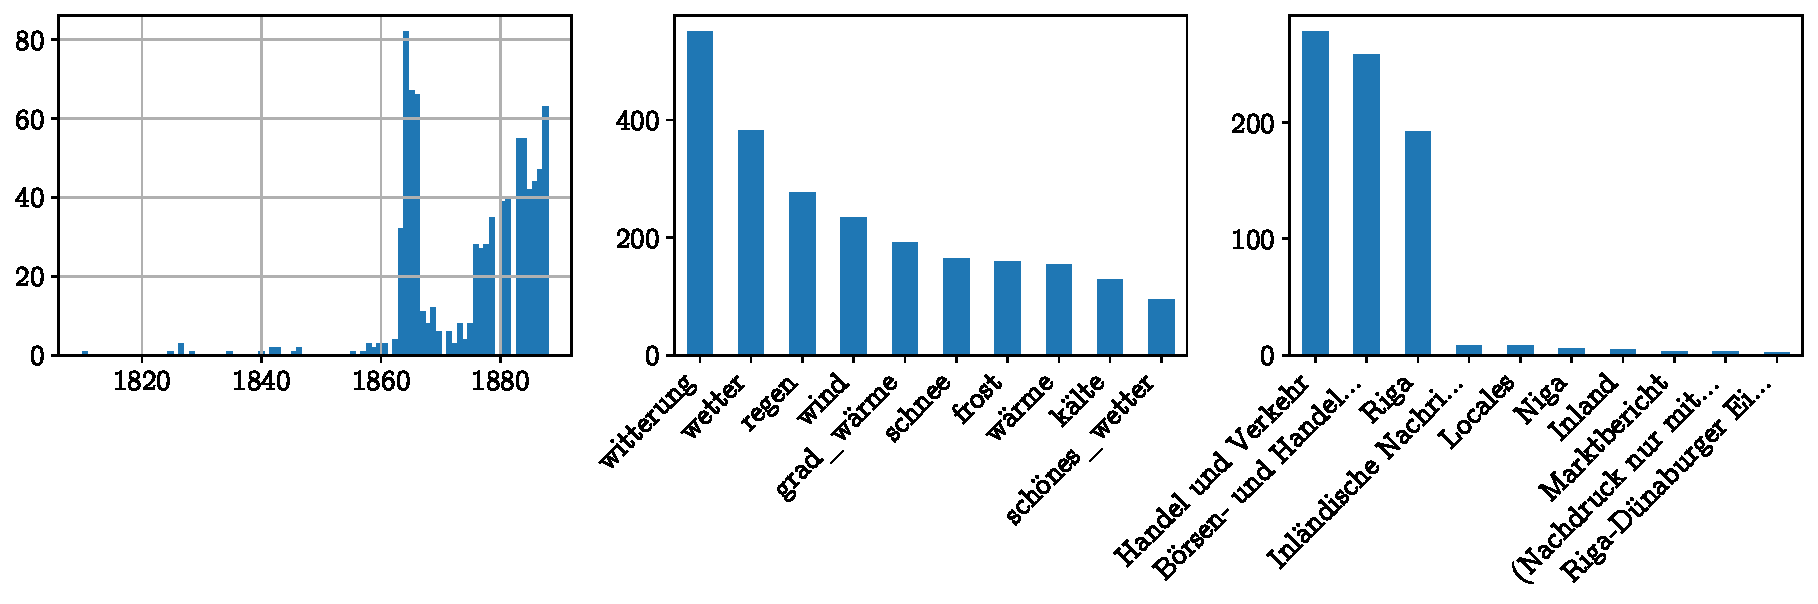
\includegraphics[width=\textwidth]{images/topic_charts_4.pdf}
\end{figure}

\begin{flushleft}
\textbf{Taille :} 848 segments

\textbf{Mots caractéristiques :} \texttt{umsatze}, \texttt{kauflust}, \texttt{bedang}, \texttt{umsatz}, \texttt{roggen\_basis}, \texttt{gedorrte}, \texttt{lieferung}, \texttt{notirungen}, \texttt{handel\_verkehr}, \texttt{umsatzen}, \texttt{loco}, \texttt{geschaft}, \texttt{hafer}, \texttt{abgeber}, \texttt{preise}, \texttt{unverandert}, \texttt{waare}, \texttt{nominell}, \texttt{kleinigkeiten}, \texttt{verkaufer}, \texttt{stimmung}, \texttt{flauer}, \texttt{roggen}, \texttt{preisen}, \texttt{ungedorrter}, \texttt{bengal}, \texttt{zufuhr}, \texttt{borsen\_handels}, \texttt{middling\_fair}, \texttt{angeboten}.
\end{flushleft}

\medskip

\noindent \textbf{Exemple :} \og Commerce et transports. Riga. 14 juin. Ces derniers jours, le temps a été variable, parfois assez frais. Le thermomètre a oscillé entre 8 et 16 degrés de chaleur. Vent de sud-ouest. L'ambiance morose se poursuit sur notre marché des céréales. Le seigle sur la base de 120 livres hollandaises s'est fait à 79 kop. par poud et ce prix serait encore à conditionner. L'avoine est faible et ne se vend pas. La marchandise séchée est proposée à 70 kop. par poud. L'orge séchée livonaise de 100 livres est vendue à 84 kop. le poud. Les graines de lin battues ne sont pas vendues en raison du manque d'offre. Quelques wagons de graines de steppe ont été vendus à 172-173 1/3 kop. le poud, ce qui a permis d'écouler les stocks. Il n'y a pas eu de nouvelles ventes de graines de chanvre. En tout, 600 bateaux sont arrivés, dont 530 en provenance de ports étrangers et 11 de ports finlandais, et 533 sont partis. \fg{}\footnote{\textit{Handel und Verkehr. Riga. 14. Juni. Die Witterung war in den letzten Tagen veränderlich, mitunter recht kühl. DaS Thermometer schwankte zwischen 8 und 16 Grad Wärme. Wind: Südwest. An unserem Getreidemarkte hält die lustlose Stimmung an. Roggen auf der Basis von 120 Pfund holländisch wurde Einiges zu 79 Kop. pro Pud gemacht und wäre dieser Preis noch zu bedingen. Hafer flau und ohne Umsatz. Gedörrte Waare wird zu 70 Kop. pro Pud angeboten. Livländische gedörrte 100pfündige Gerste bedang 84 Kop. pro Pud. Schlagkeinsamen wegen Mangels an Angebot ohne Geschäft. Einige Waggons Steppensaat wurden zu 172 bis 173 1/2 Kop. pro Pud gemacht und mit diesem Umsätze der Vorrath geräumt. Von neuen Abschlüssen in Hanfsamen ist nicht bekannt geworden. Schiffe sind im Ganzen 600, deren 530 aus ausländischen und 11 aus finnländischen Häfen angekommen und 533 ausgegangen.} RZ 14/06/1886 (\texttt{id: 277462})}



\subsection*{Navigation} \label{topic6_navigation}
\addcontentsline{toc}{subsection}{Navigation}

\begin{figure}[H]
\centering
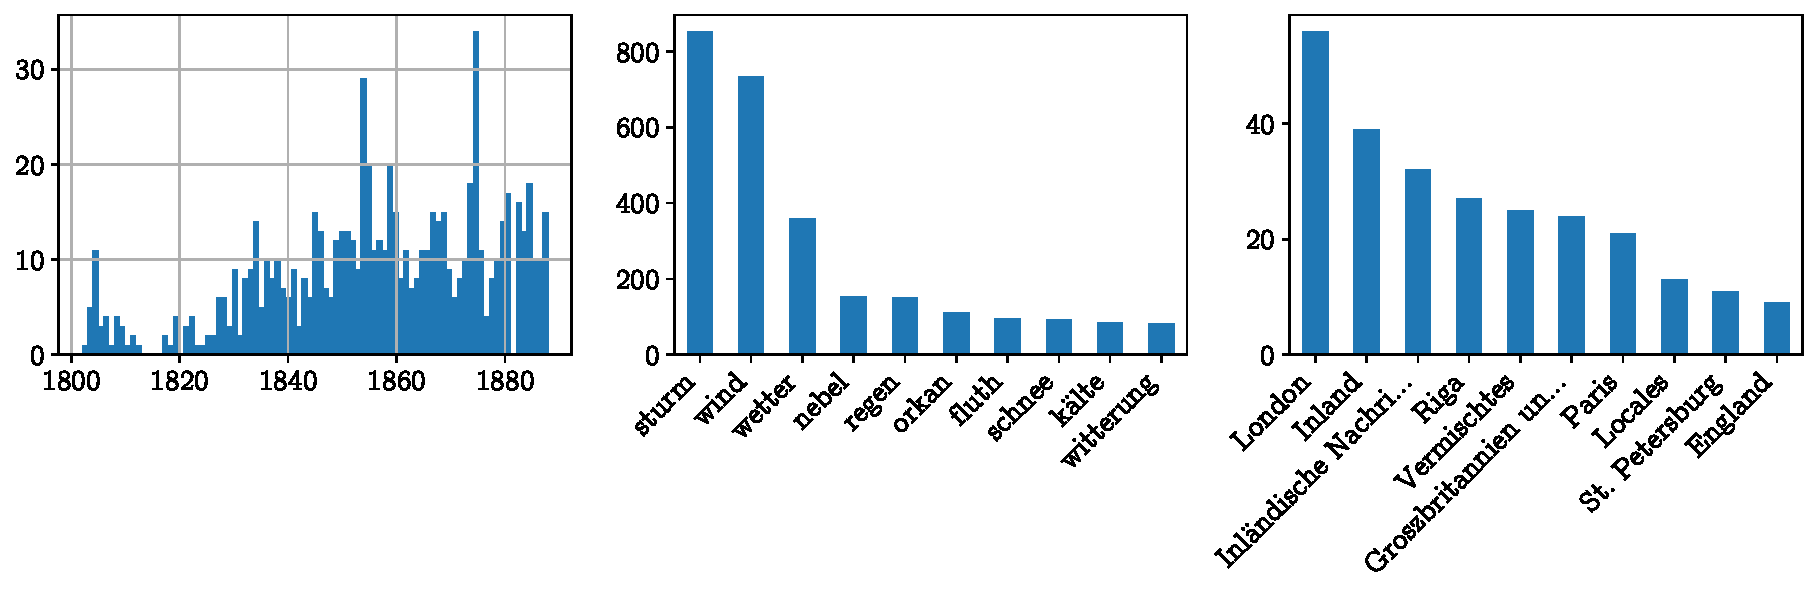
\includegraphics[width=\textwidth]{images/topic_charts_6.pdf}
\end{figure}

\begin{flushleft}
\textbf{Taille :} 734 segments

\textbf{Mots caractéristiques :} \texttt{schiff}, \texttt{schiffe}, \texttt{mannschaft}, \texttt{bord}, \texttt{anker}, \texttt{capitain}, \texttt{dampfer}, \texttt{segel}, \texttt{hafen}, \texttt{fahrzeuge}, \texttt{kuste}, \texttt{strand}, \texttt{segeln}, \texttt{ladung}, \texttt{schiffes}, \texttt{fahrzeug}, \texttt{matrosen}, \texttt{brigg}, \texttt{schiffen}, \texttt{fahrt}, \texttt{rhede}, \texttt{leck}, \texttt{wellen}, \texttt{boote}, \texttt{admiral}, \texttt{besatzung}, \texttt{dampfschiff}, \texttt{bemannung}, \texttt{deck}, \texttt{boot}.
\end{flushleft}

\medskip

\noindent \textbf{Exemple :} \og Pernau, le 9 octobre. Le 3 du mois dernier, la tempête de sud-sud-est a arraché de ses ancres le bateau-lanterne \og Julie Louise \fg{} appartenant à la maison de commerce locale Jacob Jacke \& Comp. et l'a fait dériver sur la plage à environ 4 milles de la ville. Pendant la nuit qui suivit, par une tempête orageuse et un niveau d'eau élevé (6 pieds au-dessus du niveau ordinaire), le bateau s'était couché sur le côté, et le marin et un matelot qui étaient restés sur le bateau étaient restés assis sur le mât qui dépassait de quelques brasses au-dessus de l'eau, de 10 heures du soir à 10 heures du matin le lendemain. Quatre pêcheurs tentèrent un sauvetage, mais leur bateau fut renversé par la violence des vagues, et l'un d'eux se noya à cette occasion. Les trois autres pêcheurs, ainsi que les deux personnes qui se trouvaient sur le mât, furent sauvés par plusieurs lotisseurs et matelots, au péril de leur vie. \fg{}\footnote{\textit{ Pernau, den 9. October. Durch den am 30.v.M. herrschenden SSO.-Sturm wurde das dem hiesigen Handelshause Jacob Jacke \& Comp. gehörige Lichterfahrzeug "Julie Louise" auf der Rheede von seinen Ankern gerissen und bei Kirbo circa 4 Werst von der Stadt auf den Strand getrieben. Während der darauf folgenden Nacht war bei erhöhtem orkanmäßigen Sturme und Wasserstande (6 Fuß über das gewohnliche Niveau) das Fahrzeug auf die Seite geworfen, und hatten der auf demselben zurückgebliebene
Schiffer und ein Matrose von 10 Uhr abends bis 10 Uhr vormittags des andern Tages auf dem einige Faden über dem Wasser hervorragenden Mäste gesessen. Vier Fischer machten einen Rettungsversuch, ihr Boot ward aber von der heftigen Brandung umgeworfen, bei welcher Gelegenheit einer derselben ertrank. Die drei übrigen Fischer, sowie die auf dem Mast befindlichen beiden Leute, wurden von mehrern Lootsen und Matrosen mit eigener Lebensgefahr gerettet.} RZ 21/10/1843 (\texttt{id: 72189})}

\clearpage


\subsection*{Hiver-ferroviaire} \label{topic8_hiver-ferroviaire}
\addcontentsline{toc}{subsection}{Hiver-ferroviaire}

\begin{figure}[H]
\centering
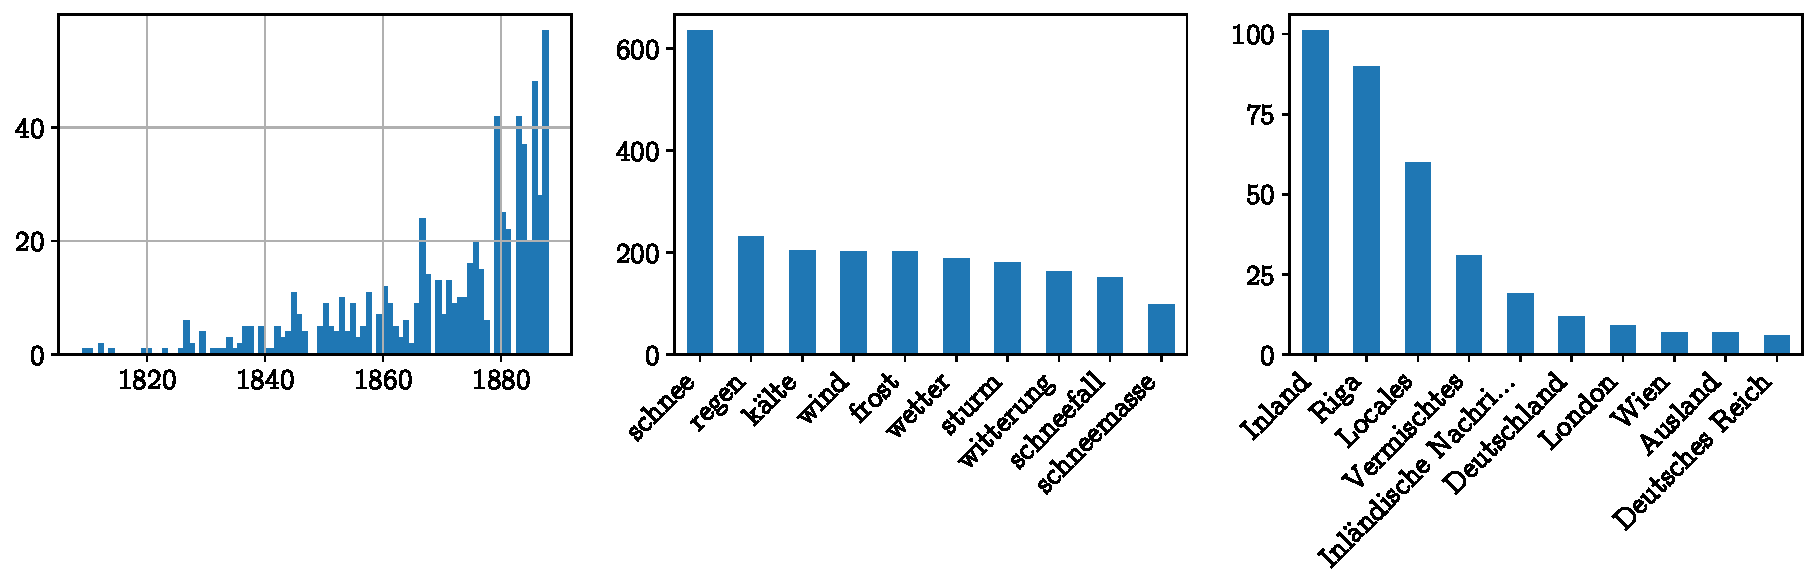
\includegraphics[width=\textwidth]{images/topic_charts_8.pdf}
\end{figure}

\begin{flushleft}
\textbf{Taille :} 677 segments

\textbf{Mots caractéristiques :} \texttt{verkehr}, \texttt{reinigung}, \texttt{strecke}, \texttt{schneemassen}, \texttt{eingestellt}, \texttt{stecken}, \texttt{zuge}, \texttt{eingesandt}, \texttt{arbeiter}, \texttt{verspatung}, \texttt{schneefall}, \texttt{straßen}, \texttt{schneemaffen}, \texttt{post}, \texttt{schneewehen}, \texttt{polizei}, \texttt{thauwetter}, \texttt{abgelassen}, \texttt{schnee}, \texttt{dirschau}, \texttt{unmoglich}, \texttt{locales}, \texttt{bahnen}, \texttt{bahn}, \texttt{communication}, \texttt{hochwasser}, \texttt{eintritt}, \texttt{locomotiven}, \texttt{schneesturme}, \texttt{waggon}.
\end{flushleft}

\medskip

\noindent \textbf{Exemple :} \og Aujourd'hui encore, nous n'avons reçu que les journaux autrichiens ; tout le reste du courrier étranger a encore manqué aujourd'hui, tant le matin qu'à midi, de sorte qu'il manque maintenant cinq ou six postes étrangers. Ce que nous publions aujourd'hui sous la rubrique \og étranger \fg{} est entièrement tiré de journaux autrichiens. D'autres villes se plaignent également des perturbations du trafic ferroviaire dues aux congères et autres phénomènes naturels. Le \og Tages.-Anz. für Libau \fg{} écrit dans son numéro d'hier : \og Entre les stations de Sehaulen, Koschedary et Dünabürg, des chutes de neige colossales ont eu lieu, ce qui a perturbé le service pendant un certain temps. Sur le chemin de fer de Varsovie, l'accumulation de neige a également entraîné des irrégularités dans le trafic \fg{}.\footnote{\textit{Heute sind uns wieder nur die österreichischen Zeitungen zugegangen; die ganze übrige ausländische Post ist sowohl Morgens als Mittags heute abermals ausgeblieben, so daß nunmehr fünf, resp. sechs ausländische Posten fehlen. Was wir heute unter der Rubrik "Ausland" bringen, ist sammt und sonders österreichischen Zeitungen entnommen. — Auch aus anderen Städten wird über Störungen des Eisenbahnverkehrs durch Schneeverwehungen und andere Naturereignisse Klage geführt. Der „Tages-Anz. für Libau" schreibt in seiner gestrigen Nummer: „Zwischen den Stationen Schaulen, Koschedary bis Dünabürg haben kolossale Schneeverwehungen stattgefunden, welche den Betrieb auf einige Zeit in's Stocken gebracht haben. Auch auf der Warschauer Bahn sind in Folge Anhäufung von Schnee Unregelmäßigkeiten im Verkehr eingetreten.} RZ 10/03/1888 (\texttt{id: 285886})}


\subsection*{Inondation} \label{topic9_inondation}
\addcontentsline{toc}{subsection}{Inondation}

\begin{figure}[H]
\centering
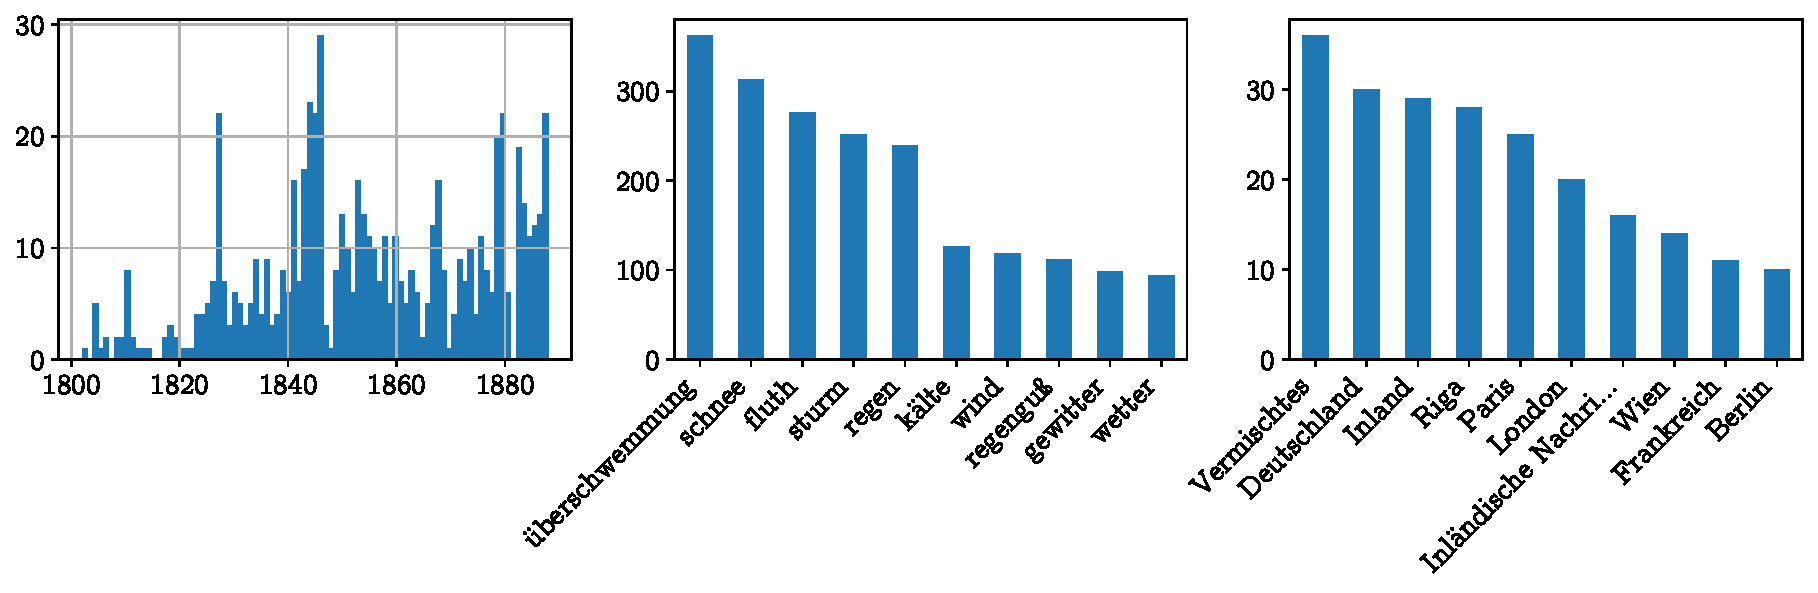
\includegraphics[width=\textwidth]{images/topic_charts_9.pdf}
\end{figure}

\begin{flushleft}
\textbf{Taille :} 657 segments

\textbf{Mots caractéristiques :} \texttt{uberschwemmt}, \texttt{uberschwemmung}, \texttt{brucken}, \texttt{ueberschwemmung}, \texttt{eingesturzt}, \texttt{weggerissen}, \texttt{fluthen}, \texttt{ortschaften}, \texttt{hauser}, \texttt{angerichtet}, \texttt{zerstort}, \texttt{fortgerissen}, \texttt{einwohner}, \texttt{menschenleben}, \texttt{straßen}, \texttt{wasser}, \texttt{heimgesucht}, \texttt{umgekommen}, \texttt{verheerungen}, \texttt{wohnungen}, \texttt{mehrere}, \texttt{verwustet}, \texttt{ungluck}, \texttt{einsturz}, \texttt{angeschwollen}, \texttt{stadt}, \texttt{uberschwemmten}, \texttt{wolkenbruch}, \texttt{unglucklichen}, \texttt{weggeschwemmt}.
\end{flushleft}

\medskip

\noindent \textbf{Exemple :} \og Lors de l'orage du 28 mai dans la région de Gladenbach, l'eau était si haute dans la localité d'Erdhausen que les personnes n'ont pu être sauvées du deuxième étage qu'au péril de leur vie. Le 1er juin, dans la région de Sauerschwabenheim, à quatre heures de Gladenbach, dans le Grand-Duché de Hesse, un terrible orage, accompagné d'une pluie torrentielle, a causé de grands ravages. Les éléments dévastateurs auraient arraché des granges, emporté le bétail hors des champs et inondé les vignes et les champs de céréales.\fg{} \footnote{\textit{Bei dem Unwetter in der Gegend von Gladenbach am 28. Mai war in dem Orte Erd-Hausen die Wassersnoth so groß, daß die Menschen nur mit größter Lebensgefahr aus dem zweiten Stockwerke gerettet werden konnten. Am 1. Juni hat in der Gegend von Sauerschwabenheim, vier Stunden von Gladenbach im Großherzogthum Hessen, ein fürchterliches Gewitter, verbunden mit einer Wolkenbruche, große Verheerungen angerichtet. Scheunen soll das verheerende Element weggerissen, das Vieh vom Felde gespült und Weingärten und Getreide-Aecker aüsgeflößt haben.} RZ 08/06/1826 (\texttt{id: 31772})}

\clearpage



\subsection*{Télégrammes} \label{topic10_télégrammes}
\addcontentsline{toc}{subsection}{Télégrammes}

\begin{figure}[H]
\centering
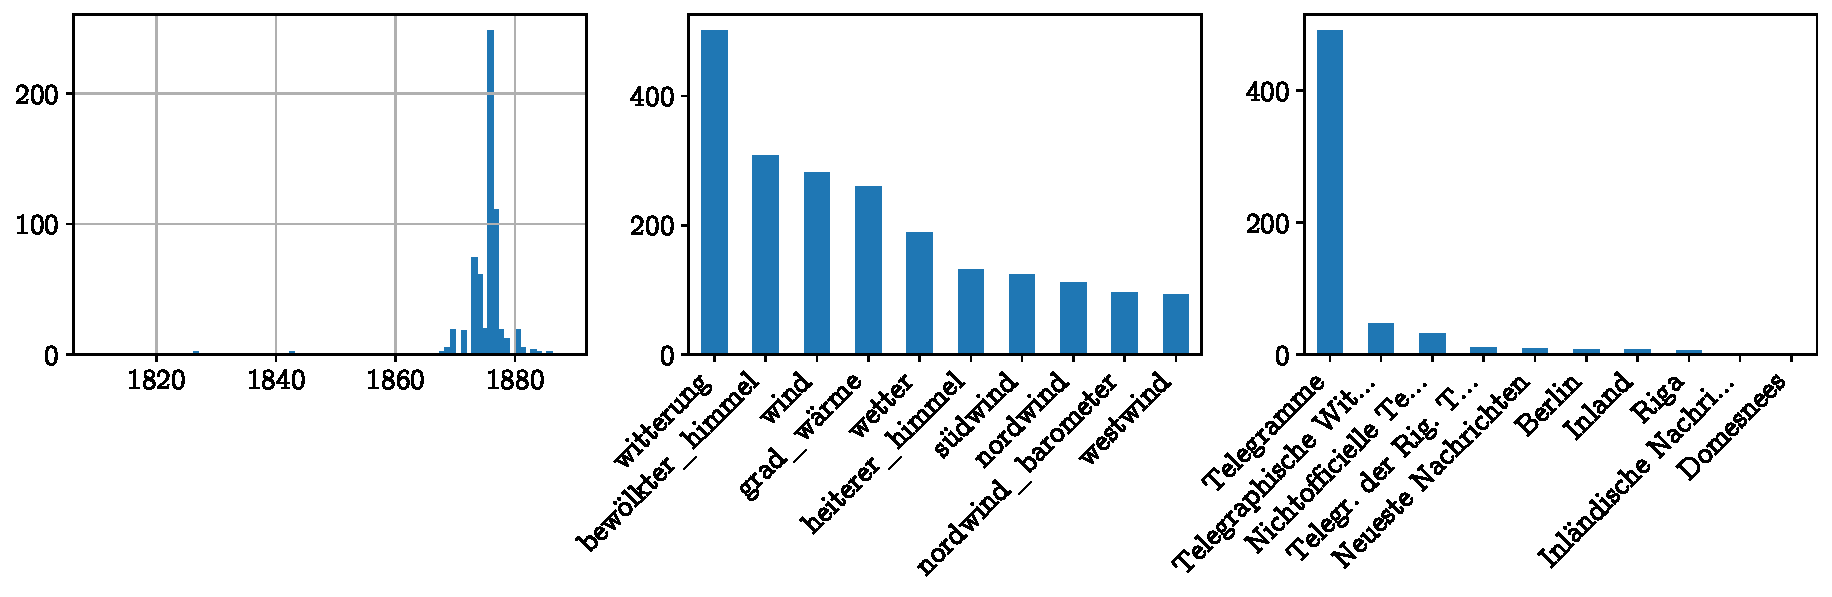
\includegraphics[width=\textwidth]{images/topic_charts_10.pdf}
\end{figure}

\begin{flushleft}
\textbf{Taille :} 640 segments

\textbf{Mots caractéristiques :} \texttt{kiew\_odessa}, \texttt{moskau\_kasan}, \texttt{grad\_archangel}, \texttt{morqens}, \texttt{uleaborg\_mill}, \texttt{petersburg}, \texttt{schwarzen\_meere}, \texttt{uleaborg}, \texttt{barometrisches}, \texttt{schwacher}, \texttt{wilna}, \texttt{weht}, \texttt{windau\_wilna}, \texttt{barometrische}, \texttt{minimum}, \texttt{belgien}, \texttt{morgens\_maßiger}, \texttt{luftdruckes}, \texttt{heiterer\_himmel}, \texttt{kuopio}, \texttt{außert}, \texttt{rußland}, \texttt{kill}, \texttt{domesnees}, \texttt{telegramm}, \texttt{archangel}, \texttt{varometer}, \texttt{maßiger}, \texttt{unbestandig}, \texttt{luftdruck}.
\end{flushleft}

\medskip

\noindent \textbf{Exemple :} \og Domesnees, le 11 mars, 9 h du matin. Vent faible du nord-ouest, baromètre le 10 mars, 9 h du soir, 29-1, le 11 mars, 9 h du matin, 29-2. Thermomètre 1 degré de gelée, ciel nuageux. Le niveau de la glace n'a pas changé. Pétersbourg, le 11 mars. (Télégramme de l'Observatoire central de physique à la station météorologique de l'Association des naturalistes à Riga). Le minimum barométrique s'est déplacé vers le lac Onega. Sur la mer Baltique et la mer Noire, le vent est faible. Dans le nord de la Russie, il neige. Au sud, le temps s'est éclairci.\fg{} \footnote{\textit{Domesnees, 11. März, 9 Uhr Morgens. Schwacher Nordwestwind, Barometer am 10. März, 9 Uhr Abends, 29—1, am 11. März, 9 Uhr Morgens. 29—2. Thermometer 1 Grad Frost, bewölkter Himmel. Der Eisstand ist unverändert. Petersburg, 11. März. (Telegramm des physikalischen Centralobservatoriums an die meteorologische Station des Naturforschervereins zu Riga.) Das barometrische Minimum hat sich nach dem Onegasee gewendet. Auf dem Baltischen und Schwarzen Meere weht der Wind schwach. Im nördlichen Rußland fällt Schnee. Im Süden hat sich die Witterung ausgeklärt.} RZ 12/03/1876 (\texttt{id: 227867})}

\clearpage


\subsection*{Tempête-grêle} \label{topic12_tempête-grêle}
\addcontentsline{toc}{subsection}{Tempête-grêle}

\begin{figure}[H]
\centering
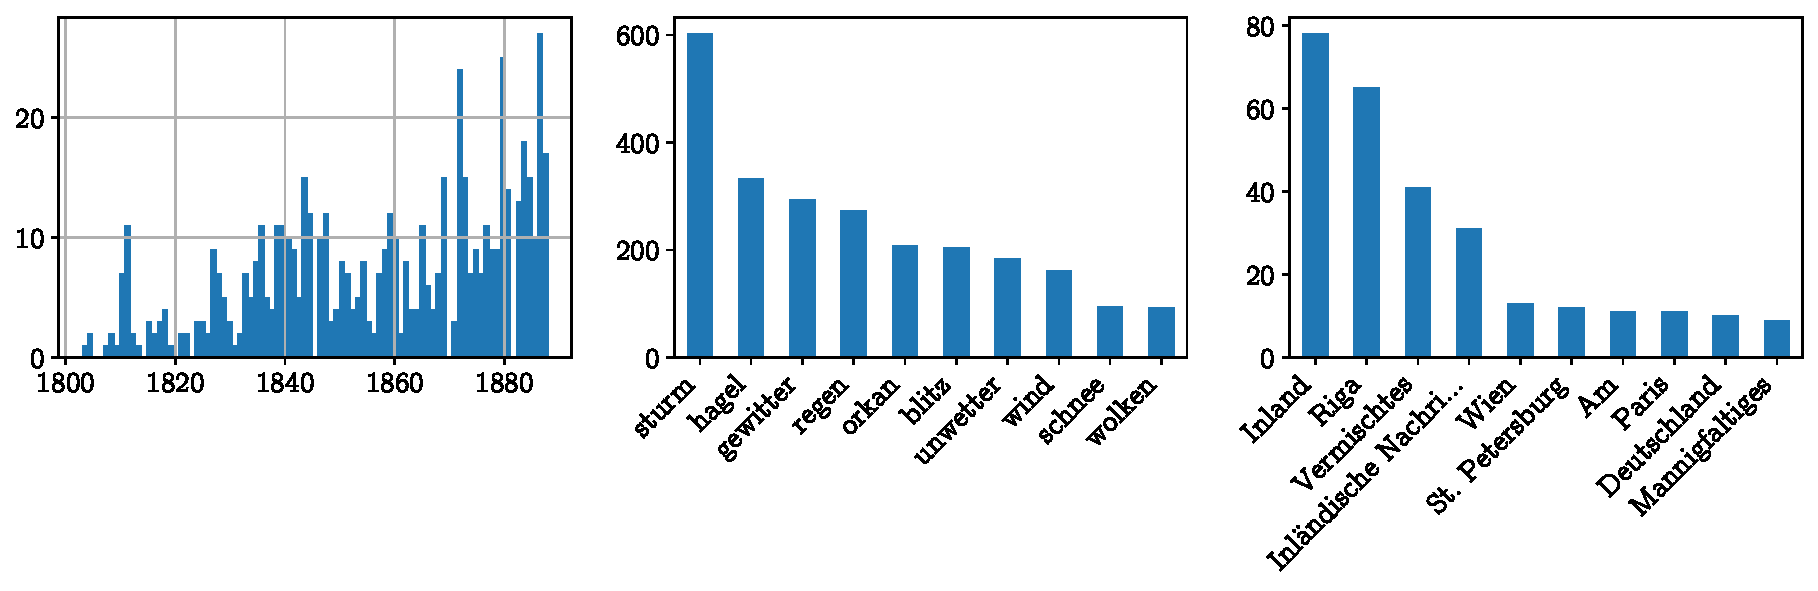
\includegraphics[width=\textwidth]{images/topic_charts_12.pdf}
\end{figure}

\begin{flushleft}
\textbf{Taille :} 591 segments

\textbf{Mots caractéristiques :} \texttt{dacher}, \texttt{entwurzelt}, \texttt{hagel}, \texttt{abgedeckt}, \texttt{angerichtet}, \texttt{orkan}, \texttt{erschlagen}, \texttt{unwetter}, \texttt{fensterscheiben}, \texttt{zerstort}, \texttt{beschadigt}, \texttt{umgeworfen}, \texttt{baume}, \texttt{zertrummert}, \texttt{verwustungen}, \texttt{gebaude}, \texttt{heimgesucht}, \texttt{schaden}, \texttt{hauser}, \texttt{vernichtet}, \texttt{umgegend}, \texttt{umgesturzt}, \texttt{gewuthet}, \texttt{mehrere}, \texttt{gerissen}, \texttt{verwustet}, \texttt{wuthete}, \texttt{anrichtete}, \texttt{windhose}, \texttt{abgerissen}.
\end{flushleft}

\medskip

\noindent \textbf{Exemple :} \og Alexin (Gouvernement de Tula), du 17 juillet. Le 17 juin, à 3 heures de l'après-midi, notre ville a subi, lors de la rencontre de deux nuages orageux, de violents éclairs, du tonnerre, des tempêtes, de la pluie et de la grêle, des dommages importants causés par cette dernière, qui a duré une heure entière, [les grêlons étaient] de la taille d'un œuf de pigeon, de poule et même d'oie, et qui a brisé les fenêtres des 5 églises locales, des locaux des autorités et de toutes les maisons. L'ouragan a arraché le toit en fer de l'église de Nikolaev, ainsi que les toits de plusieurs maisons, et en a détruit d'autres. Le toit en fer de la grande maison en pierre des marchands de la première guilde et des fabricants de Maßlow fut arraché et projeté à une demi-lieue de la maison. Les jardins fruitiers, les légumes de toutes sortes et même l'herbe ont été brisés par la grêle ; dans les environs de la ville, le seigle a été complètement détruit dans les champs sur lesquels l'orage est passé, et les paysans ont subi une perte considérable. Les grêlons pesaient jusqu'à 34 Lot [1 lb] \fg{}.\footnote{\textit{Alexin (Gouvernement Tula), vom 17. Juli. Am 17. Juni um 3 Uhr Nachmittags, litt unsere Stadt beim Zusammentreffen zweier Gewitterwolken bei heftigen Blitzen, Donner, Sturm, Regen und Hagel, einen bedeutenden Schaden durch den letztere,der eine Vollstunde anhielt, in der Größe von Tauben-, Hühner- und sogar Gänse-Eiern, und die Fenster in den 5 hiesigen Kirchen, in den Lokalen der Behörden und allen Häusern einschlug. Durch den Orkan wurden das eiserne Dach der Nikolajewschen Kirche, so wie auch die Dächer mehrerer Häuser abgerissen, andere ganz zerstört. Das eiserne Dach des großen steinernen Haused der Kaufleute Ister Gilde und Fabrikanten Maßlow wurde abgerissen und auf eine halbe Werst vom Hause geschleudert. Fruchtgärten, Gemüse aller Art und sogar Gras ward durch den Hagel zerschlagen; in den Umgegenden der Stadt ist der Roggen auf den Feldern, über die das Ungewitter zog, völlig zernichtet, und die Landleute haben einen betrachtlichen Verlust erlitten. Die Hagelkörner wogen bis 34 Loch.} RZ 17/08/1826 (\texttt{id: 31978})}

\clearpage


\subsection*{Science} \label{topic13_science}
\addcontentsline{toc}{subsection}{Science}

\begin{figure}[H]
\centering
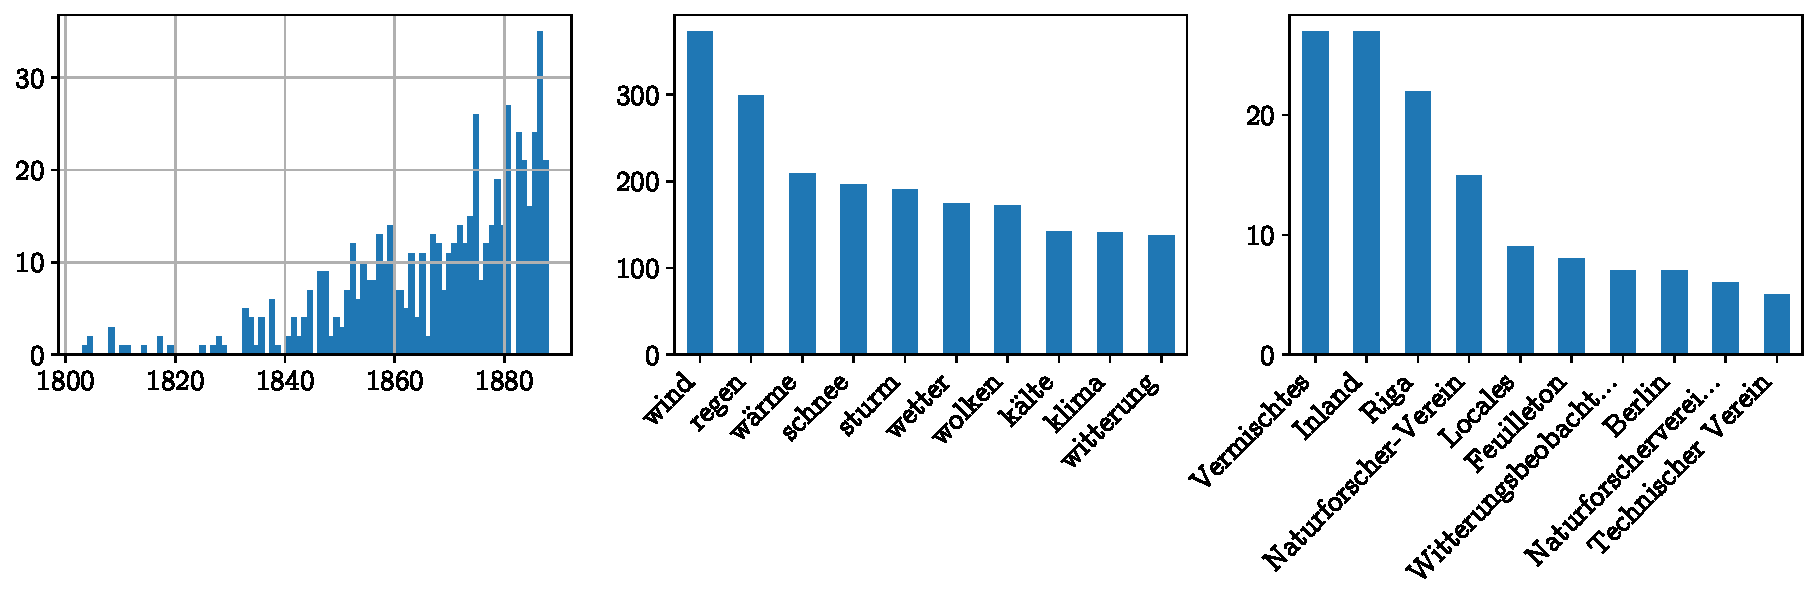
\includegraphics[width=\textwidth]{images/topic_charts_13.pdf}
\end{figure}

\begin{flushleft}
\textbf{Taille :} 576 segments

\textbf{Mots caractéristiques :} \texttt{beobachtungen}, \texttt{erscheinungen}, \texttt{erscheinung}, \texttt{beobachtet}, \texttt{erdoberflache}, \texttt{temperatur}, \texttt{ursachen}, \texttt{oberflache}, \texttt{atmosphare}, \texttt{beobachtung}, \texttt{sonne}, \texttt{beobachter}, \texttt{stromungen}, \texttt{planeten}, \texttt{atmospharischen}, \texttt{untersuchungen}, \texttt{zusammenhang}, \texttt{aequator}, \texttt{theorie}, \texttt{perioden}, \texttt{beziehung}, \texttt{niederschlage}, \texttt{einfluß}, \texttt{professor}, \texttt{periode}, \texttt{vortragende}, \texttt{meteorologie}, \texttt{erde}, \texttt{schwankungen}, \texttt{entstehen}.
\end{flushleft}

\medskip

\noindent \textbf{Exemple :} \og Glasenapp présente ici les résultats d'études sur la salinité de l'eau de la mer Baltique qu'il a effectuées en été 1876 à Bilderlingshof. Notre plage doit notamment aux vents dominants du nord-ouest le fait que, malgré la proximité de l'embouchure de Düna, la salinité de l'eau de mer y est presque aussi élevée que sur l'île d'Oesel, par exemple. En revanche, lorsque le vent souffle en sens inverse, l'eau de Düna est poussée vers les plages, ce qui réduit la salinité. Afin de clarifier cette relation, Redner mesura pendant 51 jours la salinité de l'eau et nota en même temps la direction et la force du vent, ainsi que la température de l'eau et de l'air. Les résultats de ces observations et de ces mesures ont été reportés par l'orateur sous forme graphique, la salinité, les températures et le niveau de l'eau étant représentés par des courbes, la direction et la force du vent par des flèches de direction et de longueur correspondantes.
Ce dessin, présenté à l'assemblée, montre clairement la relation entre la salinité et le vent, même s'il y a bien sûr des irrégularités et des écarts. \fg{}\footnote{\textit{Hieraus legt Glasenapp die Resultate von Untersuchungen des Salzgehalts des Ostseewassers vor, die er im Sommer 1876 bei Bilderlingshof angestellt hat.
Unser Strand hat es namentlich den vorherrschenden Nordwestwinden zu danken, daß der Salzgehalt des dortigen Seewassers trotz der Nahe der Dünamündung fast ebenso groß ist, wie z. B. bei der Insel Oesel. Dagegen wird bei entgegengesetzter Windrichtung das Dünawasser nach den Strandörtern hingetrieben und so der Salzgehalt vermindert. Um dieses Verhältniß klarzulegen, maß Redner während 51 Tage den Salzgehalt des Wassers und notirte zugleich die Richtung und Stärke des Windes, sowie die Temperatur des Wassers und der Luft. Die Resultate dieser Beobachtungen und Messungen wurden vom Redner graphisch aufgetragen, wobei der Salzgehalt, die Temperaturen und außerdem der jeweilige Wasserstand durch Curven, die Windrichtung und -Stärke dagegen durch Pfeile von entsprechender Richtung und Länge dargestellt wurden.
Aus dieser in der Versammlung vorgelegten Zeichnung ist der oben erwähnte Zusammenhang zwischen dem Salzgehalt und dem Winde besonders deutlich zu ersehen, wenn auch selbstverständlich manche Unregel-Mäßigkeiten und Abweichungen vorkommen.} RZ 29/04/1878 (\texttt{id: 240569})}



\subsection*{Düna} \label{topic14_düna}
\addcontentsline{toc}{subsection}{Düna}

\begin{figure}[H]
\centering
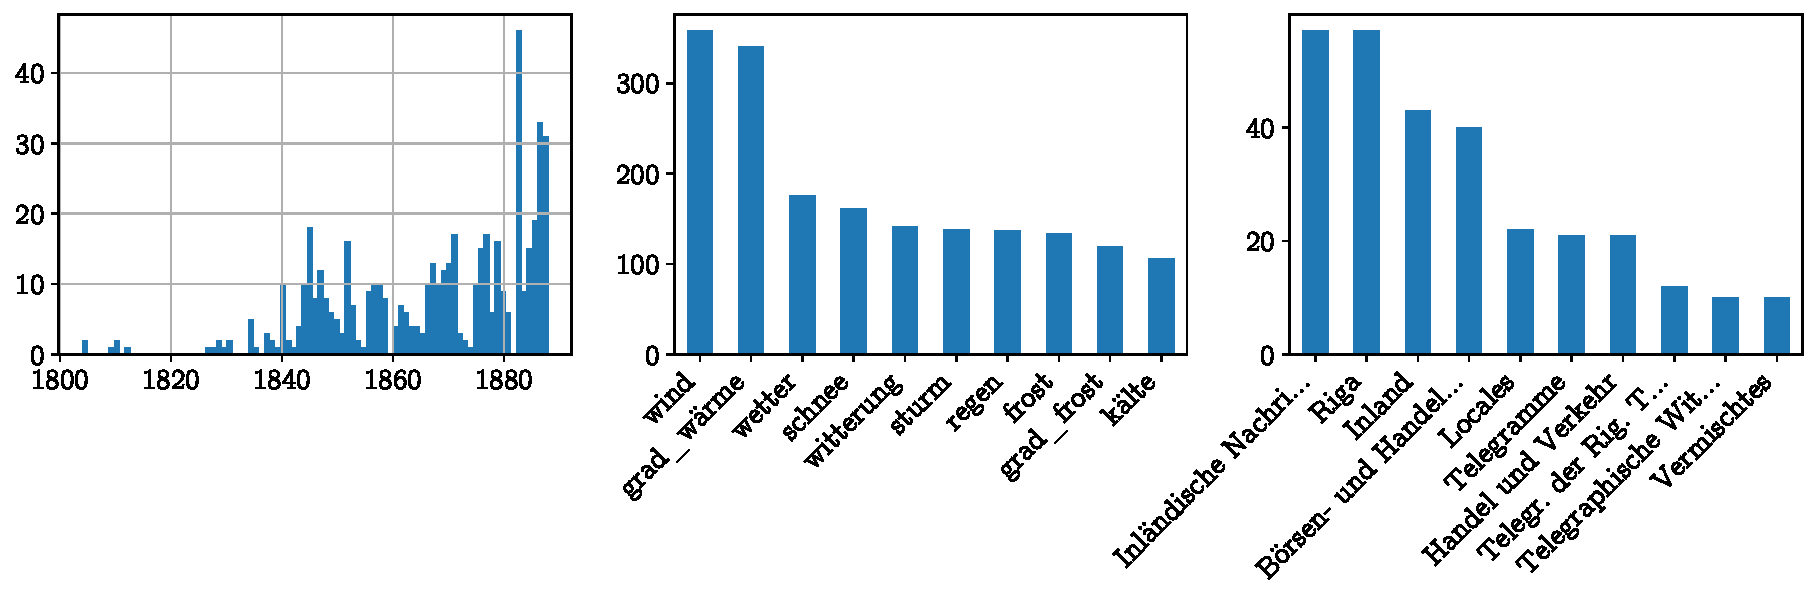
\includegraphics[width=\textwidth]{images/topic_charts_14.pdf}
\end{figure}

\begin{flushleft}
\textbf{Taille :} 516 segments

\textbf{Mots caractéristiques :} \texttt{eisfrei}, \texttt{bolderaa}, \texttt{duna}, \texttt{muhlgraben}, \texttt{eisgang}, \texttt{eisdecke}, \texttt{kreutzburg}, \texttt{fahrwasser}, \texttt{wasserstand}, \texttt{grad\_warme}, \texttt{grad\_frost}, \texttt{seegatt}, \texttt{marz}, \texttt{normal}, \texttt{passage}, \texttt{romershof}, \texttt{gestern}, \texttt{nachm}, \texttt{oger}, \texttt{morgens}, \texttt{offenes\_wasser}, \texttt{abgetrieben}, \texttt{eisstand}, \texttt{flußmundung}, \texttt{vorm}, \texttt{domesnees}, \texttt{abstromung}, \texttt{stintsee}, \texttt{rhede}, \texttt{eise}.
\end{flushleft}

\medskip

\noindent \textbf{Exemple :} \og Dünaburg, le 28 février, à 8h 1/4 du matin. Sur les rives, la glace de la Düna s'est rompue en plusieurs endroits. Par ciel clair et vent du nord, il gèle 4 degrés à l'heure. Kreutzburg, 28 février. Le matin à 9 heures. La couche de glace de la Düna est encore solide. 4 degrés de gel. Vent d'ouest.
Römershof. 28 février, matin 8 heures. Niveau de l'eau de la Düna environ 2 pieds et demi au-dessus de la normale, glace épaisse. 3 degrés de gel. Vent du sud-ouest. Oger, 28 février, 8 heures du matin. Niveau d'eau de la Düna normal, couche de glace solide, passage sans encombre. 2 degrés de gel. Vent du sud-ouest. Mühlgraben, 28 février, matin 7 h 1/2. Niveau d'eau normal. La glace de vase est debout. Gelée de 6 degrés, vent d'ouest faible. Dans la nuit, il est tombé environ 2 pouces de neige. \fg{}\footnote{\textit{Dünaburg, 28. Februar, Morgens 8 1/4 Uhr. An den Ufern ist das Eis der Düna an mehreren Stellen durchgebrochen. Bei klarem Himmel und nördlicher Windrichtung zur Stunde 4 Grad Frost.
Kreutzburg, 28. Februar. Morgens 9 Uhr. Die Eisdecke der Düna ist noch fest. 4 Grad Frost. Westwind. Römershof. 28. Februar, Morgens 8 Uhr. Wasserstand der Düna ca. 2 1/2 Fuß über normal, dichter Eisgang. 3 Grad Frost. Südwestwind. Oger, 28. Februar, Morgens 8 Uhr. Wasserstand der Düna normal, Eisdecke fest, Passage unbehindert. 2 Grad Frost. Südwestwind. Mühlgraben, 28.Februar, Morgens 7 1/2 Uhr. Wasserstand normal. Das Schlammeis steht. 6 Grad Frost, geringer Westwind. In der Nacht ist ca. 2 Zoll hoher Schnee gefallen.} RZ 28/02/1887 (\texttt{id: 280738})}

\clearpage


\subsection*{Foudre} \label{topic15_foudre}
\addcontentsline{toc}{subsection}{Foudre}

\begin{figure}[H]
\centering
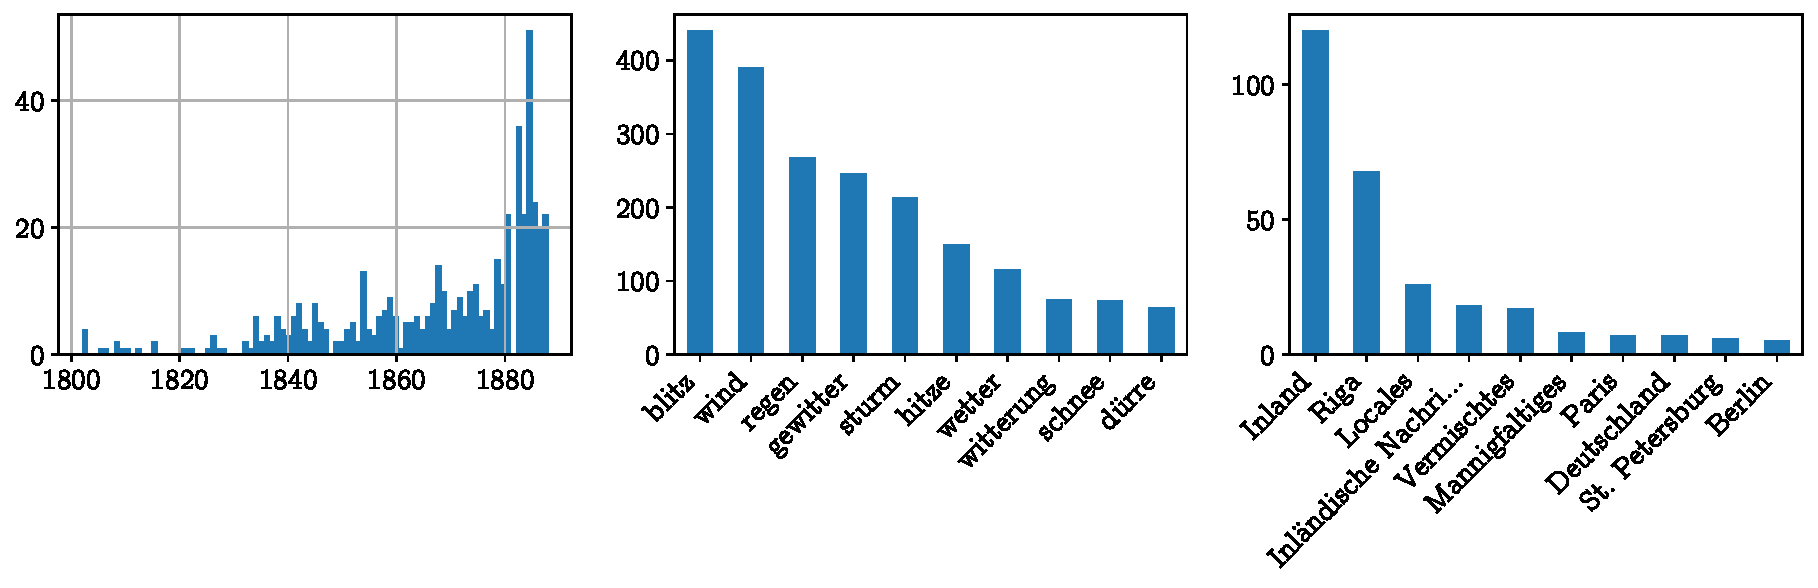
\includegraphics[width=\textwidth]{images/topic_charts_15.pdf}
\end{figure}

\begin{flushleft}
\textbf{Taille :} 497 segments

\textbf{Mots caractéristiques :} \texttt{flammen}, \texttt{feuer}, \texttt{gebaude}, \texttt{raub\_flammen}, \texttt{brand}, \texttt{feuerwehr}, \texttt{hauser}, \texttt{feuersbrunst}, \texttt{brannte}, \texttt{blitz}, \texttt{brande}, \texttt{retten}, \texttt{niedergebrannt}, \texttt{eingeaschert}, \texttt{dach}, \texttt{gesinde}, \texttt{asche\_gelegt}, \texttt{brandstatte}, \texttt{entzundete}, \texttt{brandwunden}, \texttt{haus}, \texttt{feuers}, \texttt{flamme}, \texttt{loschen}, \texttt{hause}, \texttt{schlug}, \texttt{blitzschlag}, \texttt{kirche}, \texttt{spritzen}, \texttt{brannten}.
\end{flushleft}

\medskip

\noindent \textbf{Exemple :} \og Le 30 juin, la foudre est tombée sur l'étable à bétail du ménage Dreije à Suhr et l'étable ainsi que trois trèfles ont été la proie des flammes. Le 23 juin, à 7 heures de l'après-midi, la foudre a brûlé une étable et deux granges appartenant à Uljan Allex, propriétaire de la ferme de Bewern, et à 12 heures de la nuit, la foudre a brûlé deux étables et deux granges appartenant à Jahn Tschamann, également à Bewern. Le 2 juillet, la foudre s'est abattue sur l'enclos du gardien de brousse Apscheneek et a brûlé l'enclos. Les dégâts sont estimés à 1000 roubles. Le bâtiment est assuré par l'assurance incendie de Courlande pour 60 Rbl. \fg{} \footnote{\textit{Am 30. Juni hat der Blitz in den Viehstall der Suhrschen Treije-Gefindes eingeschlagen und ist der Stall, sowie drei Kleeten ein Raub der Flammen geworden. Am 23. Juni um 7 Uhr Nachmittags hat der Blitz eine Riege und zwei Scheunen, gehörig dem unter dem Gute Bewern befindlichen Gefindes, eigenthümer Uljan Allex, und um 12 Uhr Nachts ein Blitzschlag zwei Stalle und zwei Scheunen, dem Jahn Tschamann gehörig, ebenfalls unter Bewern, eingeäschert. Am 2. Juli hat der Blitz in die Riege des Amt-Candauschen Buschwächters Apscheneek eingeschlagen und ist die Riege niedergebrannt. Der Schaden ist aus 1000 Rbl. veranschlagt. Das Gebäude ist in der Kurländischen Feuerversicherung für 60 Rbl. versichert.} RZ 11/07/1885 (\texttt{id: 273518})}


\clearpage


\section*{Code source, données et \textit{notebooks}}
\addcontentsline{toc}{section}{Code source, données et \textit{notebooks}}

\noindent \url{https://github.com/krkryger/clim-dist}

\medskip

\noindent Le corpus LNB et les modèles entraînés sont disponibles sur demande auprès de l'auteur.








\printbibliography
\addcontentsline{toc}{section}{Références}
\clearpage

\listoffigures
\clearpage

\tableofcontents
\clearpage




\end{document}
